% Generated by Sphinx.
\def\sphinxdocclass{report}
\documentclass[letterpaper,10pt,english]{sphinxmanual}
\usepackage[utf8]{inputenc}
\DeclareUnicodeCharacter{00A0}{\nobreakspace}
\usepackage{cmap}
\usepackage[T1]{fontenc}
\usepackage{babel}
\usepackage{times}
\usepackage[Bjarne]{fncychap}
\usepackage{longtable}
\usepackage{sphinx}
\usepackage{multirow}


\title{Project Report: "Be-FaVOR: Be Stars - Facilities in VO Research. Uma ferramenta para a determinação de parâmetros de estrelas Be"}
\date{November 02, 2016}
\release{1.0}
\author{Artur Alegre, Alex C. Carciofi e Bruno C. Mota}
\newcommand{\sphinxlogo}{}
\renewcommand{\releasename}{Release}
\makeindex

\makeatletter
\def\PYG@reset{\let\PYG@it=\relax \let\PYG@bf=\relax%
    \let\PYG@ul=\relax \let\PYG@tc=\relax%
    \let\PYG@bc=\relax \let\PYG@ff=\relax}
\def\PYG@tok#1{\csname PYG@tok@#1\endcsname}
\def\PYG@toks#1+{\ifx\relax#1\empty\else%
    \PYG@tok{#1}\expandafter\PYG@toks\fi}
\def\PYG@do#1{\PYG@bc{\PYG@tc{\PYG@ul{%
    \PYG@it{\PYG@bf{\PYG@ff{#1}}}}}}}
\def\PYG#1#2{\PYG@reset\PYG@toks#1+\relax+\PYG@do{#2}}

\expandafter\def\csname PYG@tok@cm\endcsname{\let\PYG@it=\textit\def\PYG@tc##1{\textcolor[rgb]{0.25,0.50,0.56}{##1}}}
\expandafter\def\csname PYG@tok@nc\endcsname{\let\PYG@bf=\textbf\def\PYG@tc##1{\textcolor[rgb]{0.05,0.52,0.71}{##1}}}
\expandafter\def\csname PYG@tok@go\endcsname{\def\PYG@tc##1{\textcolor[rgb]{0.20,0.20,0.20}{##1}}}
\expandafter\def\csname PYG@tok@vi\endcsname{\def\PYG@tc##1{\textcolor[rgb]{0.73,0.38,0.84}{##1}}}
\expandafter\def\csname PYG@tok@kn\endcsname{\let\PYG@bf=\textbf\def\PYG@tc##1{\textcolor[rgb]{0.00,0.44,0.13}{##1}}}
\expandafter\def\csname PYG@tok@sd\endcsname{\let\PYG@it=\textit\def\PYG@tc##1{\textcolor[rgb]{0.25,0.44,0.63}{##1}}}
\expandafter\def\csname PYG@tok@err\endcsname{\def\PYG@bc##1{\setlength{\fboxsep}{0pt}\fcolorbox[rgb]{1.00,0.00,0.00}{1,1,1}{\strut ##1}}}
\expandafter\def\csname PYG@tok@gt\endcsname{\def\PYG@tc##1{\textcolor[rgb]{0.00,0.27,0.87}{##1}}}
\expandafter\def\csname PYG@tok@nl\endcsname{\let\PYG@bf=\textbf\def\PYG@tc##1{\textcolor[rgb]{0.00,0.13,0.44}{##1}}}
\expandafter\def\csname PYG@tok@w\endcsname{\def\PYG@tc##1{\textcolor[rgb]{0.73,0.73,0.73}{##1}}}
\expandafter\def\csname PYG@tok@il\endcsname{\def\PYG@tc##1{\textcolor[rgb]{0.13,0.50,0.31}{##1}}}
\expandafter\def\csname PYG@tok@kt\endcsname{\def\PYG@tc##1{\textcolor[rgb]{0.56,0.13,0.00}{##1}}}
\expandafter\def\csname PYG@tok@sr\endcsname{\def\PYG@tc##1{\textcolor[rgb]{0.14,0.33,0.53}{##1}}}
\expandafter\def\csname PYG@tok@c\endcsname{\let\PYG@it=\textit\def\PYG@tc##1{\textcolor[rgb]{0.25,0.50,0.56}{##1}}}
\expandafter\def\csname PYG@tok@gi\endcsname{\def\PYG@tc##1{\textcolor[rgb]{0.00,0.63,0.00}{##1}}}
\expandafter\def\csname PYG@tok@ow\endcsname{\let\PYG@bf=\textbf\def\PYG@tc##1{\textcolor[rgb]{0.00,0.44,0.13}{##1}}}
\expandafter\def\csname PYG@tok@no\endcsname{\def\PYG@tc##1{\textcolor[rgb]{0.38,0.68,0.84}{##1}}}
\expandafter\def\csname PYG@tok@ge\endcsname{\let\PYG@it=\textit}
\expandafter\def\csname PYG@tok@cs\endcsname{\def\PYG@tc##1{\textcolor[rgb]{0.25,0.50,0.56}{##1}}\def\PYG@bc##1{\setlength{\fboxsep}{0pt}\colorbox[rgb]{1.00,0.94,0.94}{\strut ##1}}}
\expandafter\def\csname PYG@tok@c1\endcsname{\let\PYG@it=\textit\def\PYG@tc##1{\textcolor[rgb]{0.25,0.50,0.56}{##1}}}
\expandafter\def\csname PYG@tok@gp\endcsname{\let\PYG@bf=\textbf\def\PYG@tc##1{\textcolor[rgb]{0.78,0.36,0.04}{##1}}}
\expandafter\def\csname PYG@tok@k\endcsname{\let\PYG@bf=\textbf\def\PYG@tc##1{\textcolor[rgb]{0.00,0.44,0.13}{##1}}}
\expandafter\def\csname PYG@tok@s\endcsname{\def\PYG@tc##1{\textcolor[rgb]{0.25,0.44,0.63}{##1}}}
\expandafter\def\csname PYG@tok@ne\endcsname{\def\PYG@tc##1{\textcolor[rgb]{0.00,0.44,0.13}{##1}}}
\expandafter\def\csname PYG@tok@kc\endcsname{\let\PYG@bf=\textbf\def\PYG@tc##1{\textcolor[rgb]{0.00,0.44,0.13}{##1}}}
\expandafter\def\csname PYG@tok@sx\endcsname{\def\PYG@tc##1{\textcolor[rgb]{0.78,0.36,0.04}{##1}}}
\expandafter\def\csname PYG@tok@bp\endcsname{\def\PYG@tc##1{\textcolor[rgb]{0.00,0.44,0.13}{##1}}}
\expandafter\def\csname PYG@tok@nt\endcsname{\let\PYG@bf=\textbf\def\PYG@tc##1{\textcolor[rgb]{0.02,0.16,0.45}{##1}}}
\expandafter\def\csname PYG@tok@nd\endcsname{\let\PYG@bf=\textbf\def\PYG@tc##1{\textcolor[rgb]{0.33,0.33,0.33}{##1}}}
\expandafter\def\csname PYG@tok@kp\endcsname{\def\PYG@tc##1{\textcolor[rgb]{0.00,0.44,0.13}{##1}}}
\expandafter\def\csname PYG@tok@gu\endcsname{\let\PYG@bf=\textbf\def\PYG@tc##1{\textcolor[rgb]{0.50,0.00,0.50}{##1}}}
\expandafter\def\csname PYG@tok@nb\endcsname{\def\PYG@tc##1{\textcolor[rgb]{0.00,0.44,0.13}{##1}}}
\expandafter\def\csname PYG@tok@mf\endcsname{\def\PYG@tc##1{\textcolor[rgb]{0.13,0.50,0.31}{##1}}}
\expandafter\def\csname PYG@tok@nn\endcsname{\let\PYG@bf=\textbf\def\PYG@tc##1{\textcolor[rgb]{0.05,0.52,0.71}{##1}}}
\expandafter\def\csname PYG@tok@ss\endcsname{\def\PYG@tc##1{\textcolor[rgb]{0.32,0.47,0.09}{##1}}}
\expandafter\def\csname PYG@tok@mo\endcsname{\def\PYG@tc##1{\textcolor[rgb]{0.13,0.50,0.31}{##1}}}
\expandafter\def\csname PYG@tok@s1\endcsname{\def\PYG@tc##1{\textcolor[rgb]{0.25,0.44,0.63}{##1}}}
\expandafter\def\csname PYG@tok@m\endcsname{\def\PYG@tc##1{\textcolor[rgb]{0.13,0.50,0.31}{##1}}}
\expandafter\def\csname PYG@tok@mh\endcsname{\def\PYG@tc##1{\textcolor[rgb]{0.13,0.50,0.31}{##1}}}
\expandafter\def\csname PYG@tok@sc\endcsname{\def\PYG@tc##1{\textcolor[rgb]{0.25,0.44,0.63}{##1}}}
\expandafter\def\csname PYG@tok@mi\endcsname{\def\PYG@tc##1{\textcolor[rgb]{0.13,0.50,0.31}{##1}}}
\expandafter\def\csname PYG@tok@kr\endcsname{\let\PYG@bf=\textbf\def\PYG@tc##1{\textcolor[rgb]{0.00,0.44,0.13}{##1}}}
\expandafter\def\csname PYG@tok@o\endcsname{\def\PYG@tc##1{\textcolor[rgb]{0.40,0.40,0.40}{##1}}}
\expandafter\def\csname PYG@tok@vc\endcsname{\def\PYG@tc##1{\textcolor[rgb]{0.73,0.38,0.84}{##1}}}
\expandafter\def\csname PYG@tok@sh\endcsname{\def\PYG@tc##1{\textcolor[rgb]{0.25,0.44,0.63}{##1}}}
\expandafter\def\csname PYG@tok@gs\endcsname{\let\PYG@bf=\textbf}
\expandafter\def\csname PYG@tok@ni\endcsname{\let\PYG@bf=\textbf\def\PYG@tc##1{\textcolor[rgb]{0.84,0.33,0.22}{##1}}}
\expandafter\def\csname PYG@tok@gh\endcsname{\let\PYG@bf=\textbf\def\PYG@tc##1{\textcolor[rgb]{0.00,0.00,0.50}{##1}}}
\expandafter\def\csname PYG@tok@s2\endcsname{\def\PYG@tc##1{\textcolor[rgb]{0.25,0.44,0.63}{##1}}}
\expandafter\def\csname PYG@tok@nf\endcsname{\def\PYG@tc##1{\textcolor[rgb]{0.02,0.16,0.49}{##1}}}
\expandafter\def\csname PYG@tok@kd\endcsname{\let\PYG@bf=\textbf\def\PYG@tc##1{\textcolor[rgb]{0.00,0.44,0.13}{##1}}}
\expandafter\def\csname PYG@tok@sb\endcsname{\def\PYG@tc##1{\textcolor[rgb]{0.25,0.44,0.63}{##1}}}
\expandafter\def\csname PYG@tok@gr\endcsname{\def\PYG@tc##1{\textcolor[rgb]{1.00,0.00,0.00}{##1}}}
\expandafter\def\csname PYG@tok@nv\endcsname{\def\PYG@tc##1{\textcolor[rgb]{0.73,0.38,0.84}{##1}}}
\expandafter\def\csname PYG@tok@vg\endcsname{\def\PYG@tc##1{\textcolor[rgb]{0.73,0.38,0.84}{##1}}}
\expandafter\def\csname PYG@tok@si\endcsname{\let\PYG@it=\textit\def\PYG@tc##1{\textcolor[rgb]{0.44,0.63,0.82}{##1}}}
\expandafter\def\csname PYG@tok@gd\endcsname{\def\PYG@tc##1{\textcolor[rgb]{0.63,0.00,0.00}{##1}}}
\expandafter\def\csname PYG@tok@cp\endcsname{\def\PYG@tc##1{\textcolor[rgb]{0.00,0.44,0.13}{##1}}}
\expandafter\def\csname PYG@tok@se\endcsname{\let\PYG@bf=\textbf\def\PYG@tc##1{\textcolor[rgb]{0.25,0.44,0.63}{##1}}}
\expandafter\def\csname PYG@tok@na\endcsname{\def\PYG@tc##1{\textcolor[rgb]{0.25,0.44,0.63}{##1}}}

\def\PYGZbs{\char`\\}
\def\PYGZus{\char`\_}
\def\PYGZob{\char`\{}
\def\PYGZcb{\char`\}}
\def\PYGZca{\char`\^}
\def\PYGZam{\char`\&}
\def\PYGZlt{\char`\<}
\def\PYGZgt{\char`\>}
\def\PYGZsh{\char`\#}
\def\PYGZpc{\char`\%}
\def\PYGZdl{\char`\$}
\def\PYGZhy{\char`\-}
\def\PYGZsq{\char`\'}
\def\PYGZdq{\char`\"}
\def\PYGZti{\char`\~}
% for compatibility with earlier versions
\def\PYGZat{@}
\def\PYGZlb{[}
\def\PYGZrb{]}
\makeatother

\begin{document}

\maketitle
\tableofcontents
\phantomsection\label{index::doc}


O Observatório Astronômico Virtual (VO) é uma iniciativa internacional liderada pela \emph{International Virtual Observatory Alliance} (IVOA), que visa integrar, através de ferramentas interoperacionais, diferentes bancos de dados e diferentes serviços no sentido de modelos, ferramentas de análise e outros.

Neste contexto, nosso trabalho visa disponibilizar uma ferramenta de análise \emph{online} que proporcionará uma interface de integração entre o usuário e ferramentas desenvolvidas pelo grupo de pesquisa Beacon, coordenado pelo professor Dr. Alex C. Carciofi.

Esta ferramenta \emph{online} irá permitir ao usuário estimar as propriedades fundamentais básicas de estrelas Be clássicas a partir de dados fotométricos. A base para esta ferramenta são os dados disponíveis em inúmeras bases de dados do VO, bem como os códigos HDUST de transferência radiativa e o código EMCEE de minimização de múltiplos parâmetros.


\chapter{Introdução}
\label{index:introducao}\label{index:project-report-be-favor-be-stars-facilities-in-vo-research-uma-ferramenta-para-a-determinacao-de-parametros-de-estrelas-be}
Apesar de terem sido descobertas há 150 anos por Secchi 1866, estrelas Be continuam sendo verdadeiros enigmas. Estrelas Be clássicas são estrelas que apresentam a maior taxa de rotação entre as estrelas da Sequência Principal (Rivinius, Carciofi \& Martayan (2013)). Hoje, há consenso na comunidade de que a alta taxa de rotação está na base do surgimento dos efeitos peculiares apresentados por estas estrelas.

Um dos problemas centrais no estudo de estrelas do tipo Be é a obtenção de parâmetros fundamentais da estrela, tais como massa, idade, taxa de rotação e inclinação. Suas características particulares tornam essa tarefa difícil: estrelas Be são achatadas em seus polos, apresentam efeito de escurecimento gravitacional e, quando vistas de ângulos diferentes, apresentam distribuições espectrais de energia (SED) com diferentes características. A característica mais marcante, entretanto, é a presença de um disco circunstelar que altera de forma significativa o espectro estelar.

Buscando uma solução para este problema, o presente projeto visa disponibilizar à comunidade uma ferramenta no formato de um \emph{web service}, isto é, um serviço de Observatório Virtual, ligado à infraestrutura do BRAVO - \emph{Brazilian Virtual Observatory}. O método a ser utilizado por esta ferramenta baseia-se no confronto entre grades de modelos fotosféricos que levam em consideração a rotação e espectros da missão IUE, retornando dados confiáveis com estimativa de erro robusta de parâmetros estelares de uma dada lista de estrelas.


\chapter{Dados Observacionais}
\label{index:dados-observacionais}

\section{Os dados do IUE}
\label{index:os-dados-do-iue}
A missão \emph{International Ultraviolet Explorer} (IUE) foi um projeto conjunto entre NASA, ESA e PPARC. Ainda hoje este projeto é entendido como um dos telescópios astronômicos mais produtivos de todos os tempos, ultrapassando as expectativas de seus objetivos originais, dentre estes, a obtenção de espectros de alta resolução de estrelas de todos os tipos espectrais para determinar suas características físicas e fazer repetidas observações de objetos com espectros variáveis.

Os arquivos de espectros do IUE podem ser acessados no sistema da ESA chamado IUE \emph{Newly Extracted Spectra} (INES), cujo objetivo é fornecer à comunidade científica acesso aos espectros do IUE sem que se faça necessário um conhecimento técnico dos instrumentos. Para informações detalhadas sobre o sistema, veja \href{http://sdc.cab.inta-csic.es/ines}{http://sdc.cab.inta-csic.es/ines}.


\section{O \emph{Web Service}}
\label{index:o-web-service}
A ferramenta em desenvolvimento utilizará como \emph{input} o nome de uma estrela para automaticamente baixar os dados do repositório \emph{online} do INES e de outros serviços disponíveis e graficá-los de forma pré-derterminada. Desta maneira, não será necessário o usuário baixar os dados das estrelas que deseja estudar em seu computador, selecioná-los e, então, enviá-los de volta ao servidor para serem analisados; bastará apenas selecionar os espectros com os quais deseja trabalhar.

Para construir esta ferramenta, o projeto foi dividido em duas etapas:
\begin{enumerate}
\item {} 
Elaboração de uma rotina capaz de ler os dados observacionais diretamente através do servidor.
\begin{quote}

Esta rotina é a responsável por fazer o \emph{download} automático dos dados buscando no servidor pelo nome da estrela.
\end{quote}

\item {} 
Implementação da rotina Python de determinação dos parâmetros estelares.
\begin{quote}

Esta parte inclui a criação de uma interface que permita ao usuário executar as rotinas de interesse dentro de um ambiente de VO.
\end{quote}

\end{enumerate}

Este serviço será hospedado na \emph{homepage} do grupo Beacon, ao lado de outro projeto que visamos integrar ao BRAVO, o BEATLAS (Faes et al. 2017 in prep.), ferramenta que colocará à disposição da comunidade cerca de 70.000 espectros sintéticos de estrelas Be.


\chapter{Ferramentas}
\label{index:ferramentas}
Nesta seção, são descritas as rotinas Python criadas para leitura dos dados através do servidor: BeFaVOR-Web e TAKE-VIZIER-DATA. Esta última trata-se de uma rotina complementar para habilitar a primeira a buscar por múltiplas estrelas de uma vez.


\section{BeFaVOR-Web}
\label{index:befavor-web}
A rotina BeFaVOR-Web usa como \emph{input} tanto o nome de uma única estrela quanto uma lista de estrelas para realizar uma busca por arquivos de espectros correspondentes no \emph{database} do sistema INES, salvando-os na pasta definida. Em seguida, realiza-se, para a mesma estrela, uma busca no SIMBAD, através do qual obtemos os parâmetros: paralaxe, vsini e suas respectivas incertezas, além da referência bibliográfica para vsini. Também é verificado se a busca na plataforma IRSA-\emph{Galactic DUST Reddening \& Extinction} retorna algum valor de avermelhamento E(B-V) para aquela estrela. Caso positivo, o valor é salvo juntamente com os outros parâmetros em uma tabela na pasta definida.


\subsection{Instalação}
\label{index:instalacao}
Para utilizar esta rotina em sua atual versão é preciso ter instalados os seguintes pacotes:
\begin{quote}
\begin{enumerate}
\item {} 
numpy

\item {} 
bs4

\item {} 
datetime

\item {} 
requests

\item {} 
selenium

\item {} 
astroquery

\item {} 
pyhdust

\item {} 
matplotlib

\end{enumerate}
\begin{enumerate}
\setcounter{enumi}{8}
\item {} 
urllib

\item {} 
re

\item {} 
random

\item {} 
tafile

\end{enumerate}
\end{quote}

Os pacotes numerados de 1 a 8 podem ser instalados utilizando o gerenciador de pacotes \textbf{pip}, enquanto aqueles de 9 a 12 podem ser instalados pelo comando \textbf{apt-get install python3-pacote}.


\subsection{Executando a BeFaVOR-Web}
\label{index:executando-a-befavor-web}
Para rodar a rotina o usuário deve primeiro definir o \emph{path} onde esta encontra-se instalada na tag \textbf{commum\_folder}, bem como o \emph{path} onde as tabelas serão salvas em \textbf{folder\_tables}. Recomenda-se utilizar a versão mais atual disponível do Python.

Utilizando como exemplo o IPython 3.0, o código pode ser rodado seguindo os seguintes passos:
\begin{enumerate}
\item {} 
Abra o terminal e digite o comando:  ipython3

\item {} 
Vá ao diretório em que a rotina encontra-se instalada;

\item {} 
No terminal, digite o comando:   run BeFaV0r\_web.py

\item {} 
A rotina perguntará se o usuário deseja buscar apenas um ou vários alvos. Digite `1' para buscar um único alvo ou `more' para buscar múltiplos alvos;

\item {} 
Caso tenha digitado `1', a rotina perguntará o nome do alvo. Digite o nome da estrela desejada;

\item {} 
Caso tenha digitado `more' a rotina executará a rotina complementar TAKE\_VIZIER\_DATA que baixará uma série de alvos de acordo com um catálogo pré-definido. Para mais detalhes, veja a descrição da rotina TAKE\_VIZIER\_DATA na sub-seção seguinte.

\end{enumerate}

Se o usuário tiver buscado por um único alvo, além dos espectros do IUE salvos, a rotina criará um documento de texto com a seguinte estrutura de \textbf{linhas}:
\begin{enumerate}
\item {} 
Nome da estrela

\item {} 
Paralaxe

\item {} 
Incerteza da paralaxe

\item {} 
vsini

\item {} 
Incerteza do vsini

\item {} 
``Bump''

\item {} 
Referência bibliográfica do vsini

\item {} 
E(B-V)

\end{enumerate}

``Bump'' refere-se à presença de um espectro IUE que cobre a região conhecida como \emph{bump} 2200 Angstron que é utiliza na determinação do valor de E(B-V). Caso retorne ``\emph{True}'', existe este espectro e, caso retorne ``\emph{False}'', significa que o espectro não cobre esta faixa espectral e, portanto, o valor é retirado do IRSA.

Se o usuário tiver buscado por múltiplos alvos, além dos espectros do IUE salvos, a rotina criará um documento de texto com uma estrutura de \textbf{colunas} pré-determinada pelo usuário. Por exemplo, caso o usuário selecione estrelas do \emph{Bright Star Catalogue}, é possível gerar a seguinte estrutura:
\begin{enumerate}
\item {} 
Nome da estrela

\item {} 
Índice B-V

\item {} 
Índice U-B

\item {} 
Índice R-I

\item {} 
vsini

\item {} 
Incerteza B-V

\item {} 
Incerteza U-B

\item {} 
Incerteza vsini

\item {} 
Incerteza R-I

\item {} 
Data de observação

\item {} 
Tipo espectral

\end{enumerate}


\subsection{Funções da rotina BeFaVOR-Web}
\label{index:funcoes-da-rotina-befavor-web}
Segue a descrição das funções contidas na rotina BeFaVOR-Web, organizadas em ordem alfabética:
\phantomsection\label{index:module-BeFaVOr_web}\index{BeFaVOr\_web (module)}\index{create\_list\_files() (in module BeFaVOr\_web)}

\begin{fulllineitems}
\phantomsection\label{index:BeFaVOr_web.create_list_files}\pysiglinewithargsret{\code{BeFaVOr\_web.}\bfcode{create\_list\_files}}{\emph{list\_name}, \emph{folder}, \emph{folder\_table}}{}
Creates a list of the files inside a given folder.
\begin{quote}\begin{description}
\item[{Parameters}] \leavevmode\begin{itemize}
\item {} 
\textbf{list\_name} -- list's name (string)

\item {} 
\textbf{folder} -- files' folder (string)

\end{itemize}

\item[{Returns}] \leavevmode
creates a txt file, with the files' paths

\end{description}\end{quote}

\end{fulllineitems}

\index{create\_txt\_file() (in module BeFaVOr\_web)}

\begin{fulllineitems}
\phantomsection\label{index:BeFaVOr_web.create_txt_file}\pysiglinewithargsret{\code{BeFaVOr\_web.}\bfcode{create\_txt\_file}}{\emph{data\_list}, \emph{file\_name}}{}
Create a txt file.
\begin{quote}\begin{description}
\item[{Parameters}] \leavevmode\begin{itemize}
\item {} 
\textbf{data\_list} -- list of data to be saved (array)

\item {} 
\textbf{file\_name} -- txt file's name (string)

\end{itemize}

\item[{Returns}] \leavevmode
txt file

\end{description}\end{quote}

\end{fulllineitems}

\index{find\_regular\_expression() (in module BeFaVOr\_web)}

\begin{fulllineitems}
\phantomsection\label{index:BeFaVOr_web.find_regular_expression}\pysiglinewithargsret{\code{BeFaVOr\_web.}\bfcode{find\_regular\_expression}}{\emph{url}, \emph{typ}, \emph{atr}, \emph{expr}}{}
Search for a specified expression inside a page code and lists all
its ocurrences.
\begin{quote}\begin{description}
\item[{Parameters}] \leavevmode\begin{itemize}
\item {} 
\textbf{url} -- page url (string)

\item {} 
\textbf{typ} -- tag (string)

\item {} 
\textbf{atr} -- attribute (string)

\item {} 
\textbf{expr} -- expression (string)

\end{itemize}

\item[{Returns}] \leavevmode
list of occurences

\end{description}\end{quote}

\end{fulllineitems}

\index{getTitle() (in module BeFaVOr\_web)}

\begin{fulllineitems}
\phantomsection\label{index:BeFaVOr_web.getTitle}\pysiglinewithargsret{\code{BeFaVOr\_web.}\bfcode{getTitle}}{\emph{url}}{}
Gets the title of a certain webpage.
\begin{quote}\begin{description}
\item[{Parameters}] \leavevmode
\textbf{url} -- page url (string)

\item[{Returns}] \leavevmode
page title

\end{description}\end{quote}

\end{fulllineitems}

\index{get\_attribute() (in module BeFaVOr\_web)}

\begin{fulllineitems}
\phantomsection\label{index:BeFaVOr_web.get_attribute}\pysiglinewithargsret{\code{BeFaVOr\_web.}\bfcode{get\_attribute}}{\emph{url}, \emph{atr}, \emph{typ}}{}
Lists all text in a webpage that satisfacts a specified attribute.
\begin{quote}\begin{description}
\item[{Parameters}] \leavevmode\begin{itemize}
\item {} 
\textbf{url} -- page url (string)

\item {} 
\textbf{atr} -- attribute (string)

\item {} 
\textbf{typ} -- tag (string)

\end{itemize}

\item[{Returns}] \leavevmode
text containing specified attribute

\end{description}\end{quote}

\end{fulllineitems}

\index{iue\_submission() (in module BeFaVOr\_web)}

\begin{fulllineitems}
\phantomsection\label{index:BeFaVOr_web.iue_submission}\pysiglinewithargsret{\code{BeFaVOr\_web.}\bfcode{iue\_submission}}{\emph{star\_name}}{}
Search in the IUE database for a certain star name.
\begin{quote}\begin{description}
\item[{Parameters}] \leavevmode
\textbf{star\_name} -- name of the star (string)

\item[{Returns}] \leavevmode
request of star name in IUE page

\end{description}\end{quote}

\end{fulllineitems}

\index{plot\_gal() (in module BeFaVOr\_web)}

\begin{fulllineitems}
\phantomsection\label{index:BeFaVOr_web.plot_gal}\pysiglinewithargsret{\code{BeFaVOr\_web.}\bfcode{plot\_gal}}{\emph{ra\_val}, \emph{dec\_val}, \emph{folder\_fig}}{}
Plot in ``Galatic Coordinates'' (i.e., Mollweide projection).
\begin{quote}\begin{description}
\item[{Parameters}] \leavevmode\begin{itemize}
\item {} 
\textbf{ra\_val} -- right ascencion in RADIANS (float)

\item {} 
\textbf{dec\_val} -- declination in RADIANS (float)

\item {} 
\textbf{folder\_fig} -- name of the folder for the figure (string)

\end{itemize}

\item[{Returns}] \leavevmode
saved images

\end{description}\end{quote}

\end{fulllineitems}

\index{read\_simbad\_coodr() (in module BeFaVOr\_web)}

\begin{fulllineitems}
\phantomsection\label{index:BeFaVOr_web.read_simbad_coodr}\pysiglinewithargsret{\code{BeFaVOr\_web.}\bfcode{read\_simbad\_coodr}}{\emph{star\_name}}{}
Query SIMBAD for the coordinates of a given star.
\begin{quote}\begin{description}
\item[{Parameters}] \leavevmode
\textbf{star\_name} -- star's name (string)

\item[{Returns}] \leavevmode
right ascencion and declination coordinates

\end{description}\end{quote}

\end{fulllineitems}

\index{read\_simbad\_data() (in module BeFaVOr\_web)}

\begin{fulllineitems}
\phantomsection\label{index:BeFaVOr_web.read_simbad_data}\pysiglinewithargsret{\code{BeFaVOr\_web.}\bfcode{read\_simbad\_data}}{\emph{star\_name}}{}
Query SIMBAD for a given star parallax, vsini, bump and references.
\begin{quote}\begin{description}
\item[{Parameters}] \leavevmode
\textbf{star\_name} -- star's name (string)

\item[{Returns}] \leavevmode
txt file with star's parallax, vsini, bump, the respective

\end{description}\end{quote}

errors and references for vsini and E(B-V)

\end{fulllineitems}

\index{read\_txt() (in module BeFaVOr\_web)}

\begin{fulllineitems}
\phantomsection\label{index:BeFaVOr_web.read_txt}\pysiglinewithargsret{\code{BeFaVOr\_web.}\bfcode{read\_txt}}{\emph{list\_name}, \emph{folder}}{}
Read a given list of star names.
\begin{quote}\begin{description}
\item[{Parameters}] \leavevmode\begin{itemize}
\item {} 
\textbf{list\_name} -- name o txt file containing the list (string)

\item {} 
\textbf{folder} -- list's folder (string)

\end{itemize}

\item[{Returns}] \leavevmode
column of the list read

\end{description}\end{quote}

\end{fulllineitems}

\index{retrieve\_ebmv\_value() (in module BeFaVOr\_web)}

\begin{fulllineitems}
\phantomsection\label{index:BeFaVOr_web.retrieve_ebmv_value}\pysiglinewithargsret{\code{BeFaVOr\_web.}\bfcode{retrieve\_ebmv\_value}}{\emph{star\_name}}{}
Search the INES website for a specified star's E(B-V) value.
\begin{quote}\begin{description}
\item[{Parameters}] \leavevmode
\textbf{star\_name} -- stars's name (string)

\item[{Returns}] \leavevmode
E(B-V) value

\end{description}\end{quote}

\end{fulllineitems}

\index{selecting\_data() (in module BeFaVOr\_web)}

\begin{fulllineitems}
\phantomsection\label{index:BeFaVOr_web.selecting_data}\pysiglinewithargsret{\code{BeFaVOr\_web.}\bfcode{selecting\_data}}{\emph{star\_name}, \emph{commum\_folder}}{}
Search the INES website for a specified star.
\begin{quote}\begin{description}
\item[{Parameters}] \leavevmode\begin{itemize}
\item {} 
\textbf{star\_name} -- name of the star (string)

\item {} 
\textbf{commum\_folder} -- name of the folder where the routine is located

\end{itemize}

\item[{Returns}] \leavevmode
request of the star name in INES page

\end{description}\end{quote}

\end{fulllineitems}

\index{show\_page\_code() (in module BeFaVOr\_web)}

\begin{fulllineitems}
\phantomsection\label{index:BeFaVOr_web.show_page_code}\pysiglinewithargsret{\code{BeFaVOr\_web.}\bfcode{show\_page\_code}}{\emph{url}}{}
Shows the page code of a certain webpage.
\begin{quote}\begin{description}
\item[{Parameters}] \leavevmode
\textbf{url} -- page url (string)

\item[{Returns}] \leavevmode
page code

\end{description}\end{quote}

\end{fulllineitems}

\index{there\_is\_a\_title() (in module BeFaVOr\_web)}

\begin{fulllineitems}
\phantomsection\label{index:BeFaVOr_web.there_is_a_title}\pysiglinewithargsret{\code{BeFaVOr\_web.}\bfcode{there\_is\_a\_title}}{\emph{url}}{}
Prints the title of a certain webpage.
\begin{quote}\begin{description}
\item[{Parameters}] \leavevmode
\textbf{url} -- page url (string)

\item[{Returns}] \leavevmode
page title

\end{description}\end{quote}

\end{fulllineitems}

\index{untar() (in module BeFaVOr\_web)}

\begin{fulllineitems}
\phantomsection\label{index:BeFaVOr_web.untar}\pysiglinewithargsret{\code{BeFaVOr\_web.}\bfcode{untar}}{\emph{fname}}{}
Decompact a tar file.
\begin{quote}\begin{description}
\item[{Parameters}] \leavevmode
\textbf{fname} -- name o file to be decompacted (string)

\item[{Returns}] \leavevmode
decompacted file

\end{description}\end{quote}

\end{fulllineitems}

\index{unzip() (in module BeFaVOr\_web)}

\begin{fulllineitems}
\phantomsection\label{index:BeFaVOr_web.unzip}\pysiglinewithargsret{\code{BeFaVOr\_web.}\bfcode{unzip}}{\emph{zip\_file}, \emph{outdir}}{}
Unzip a given file into the specified output directory.
\begin{quote}\begin{description}
\item[{Parameters}] \leavevmode\begin{itemize}
\item {} 
\textbf{zip\_file} -- name of file to be unziped (string)

\item {} 
\textbf{outdir} -- directory of the file (string)

\end{itemize}

\item[{Returns}] \leavevmode
unziped file

\end{description}\end{quote}

\end{fulllineitems}



\section{TAKE-VIZIER-DATA}
\label{index:take-vizier-data}
A rotina TAKE-VIZIER-DATA realiza uma busca por catálogos no VizieR. Em seguida, dentro de cada catálogo selecionado, é feita a seleção dos objetos de interesse através de um processo de filtragem por tipo espectral, classe de luminosidade e existência ou não de dados da missão IUE. Deste ponto em diante, a rotina segue os seguintes passos:
\begin{enumerate}
\item {} 
As estrelas selecionadas no VizieR são buscadas no arquivo do INES;

\item {} 
Os espectros daquelas encontradas são salvos no diretório definido;

\item {} 
Para cada estrela encontrada no INES, é criado um documento de texto onde são salvos os parâmetros retirados do SIMBAD e (opcional) os parâmetros obtidos dos catálogos lidos por meio do VIZIER.

\end{enumerate}

Detalhes sobre as funções contidas nesta rotina podem ser vistos no anexo do capítulo 6.


\chapter{Outras Atividades e Perspectivas}
\label{index:outras-atividades-e-perspectivas}

\section{Atividades complementares}
\label{index:atividades-complementares}
Ao longo do período de duração desta bolsa, além das tarefas diretamente relacionadas a este projeto, também foram realizadas atividades importantes para o desenvolvimento acadêmico, dentre elas destacamos:
\begin{enumerate}
\item {} 
Participação de reuniões semanais do grupo Beacon, onde são discutidos resultados recentes das pesquisas de seus membros, bem como artigos científicos relevantes para nossa linha de pesquisa;

\item {} 
Apresentação de resultados parciais deste projeto na reunião de grupo;

\item {} 
Participação de observações astronômicas tanto remotas quanto presenciais no Observatório Pico dos Dias para obtenção de dados polarimétricos e espectroscópicos.

\end{enumerate}


\section{Tarefas futuras}
\label{index:tarefas-futuras}\begin{enumerate}
\item {} 
Incorporação das rotinas de leitura de dados em servidores desenvolvidas neste projeto com a rotina Python de determinação de parâmetros estelares que constitui parte do projeto de doutorado do aluno Bruno C. Mota.

\item {} 
Desenvolvimento e integração, na \emph{homepage} do grupo Beacon, da interface que permitirá ao usuário executar as rotinas Python criadas ao longo ou anteriormente a este projeto em um ambiente de Observatório Virtual.

\end{enumerate}


\chapter{Conclusões}
\label{index:conclusoes}\begin{figure}[htbp]
\centering
\capstart

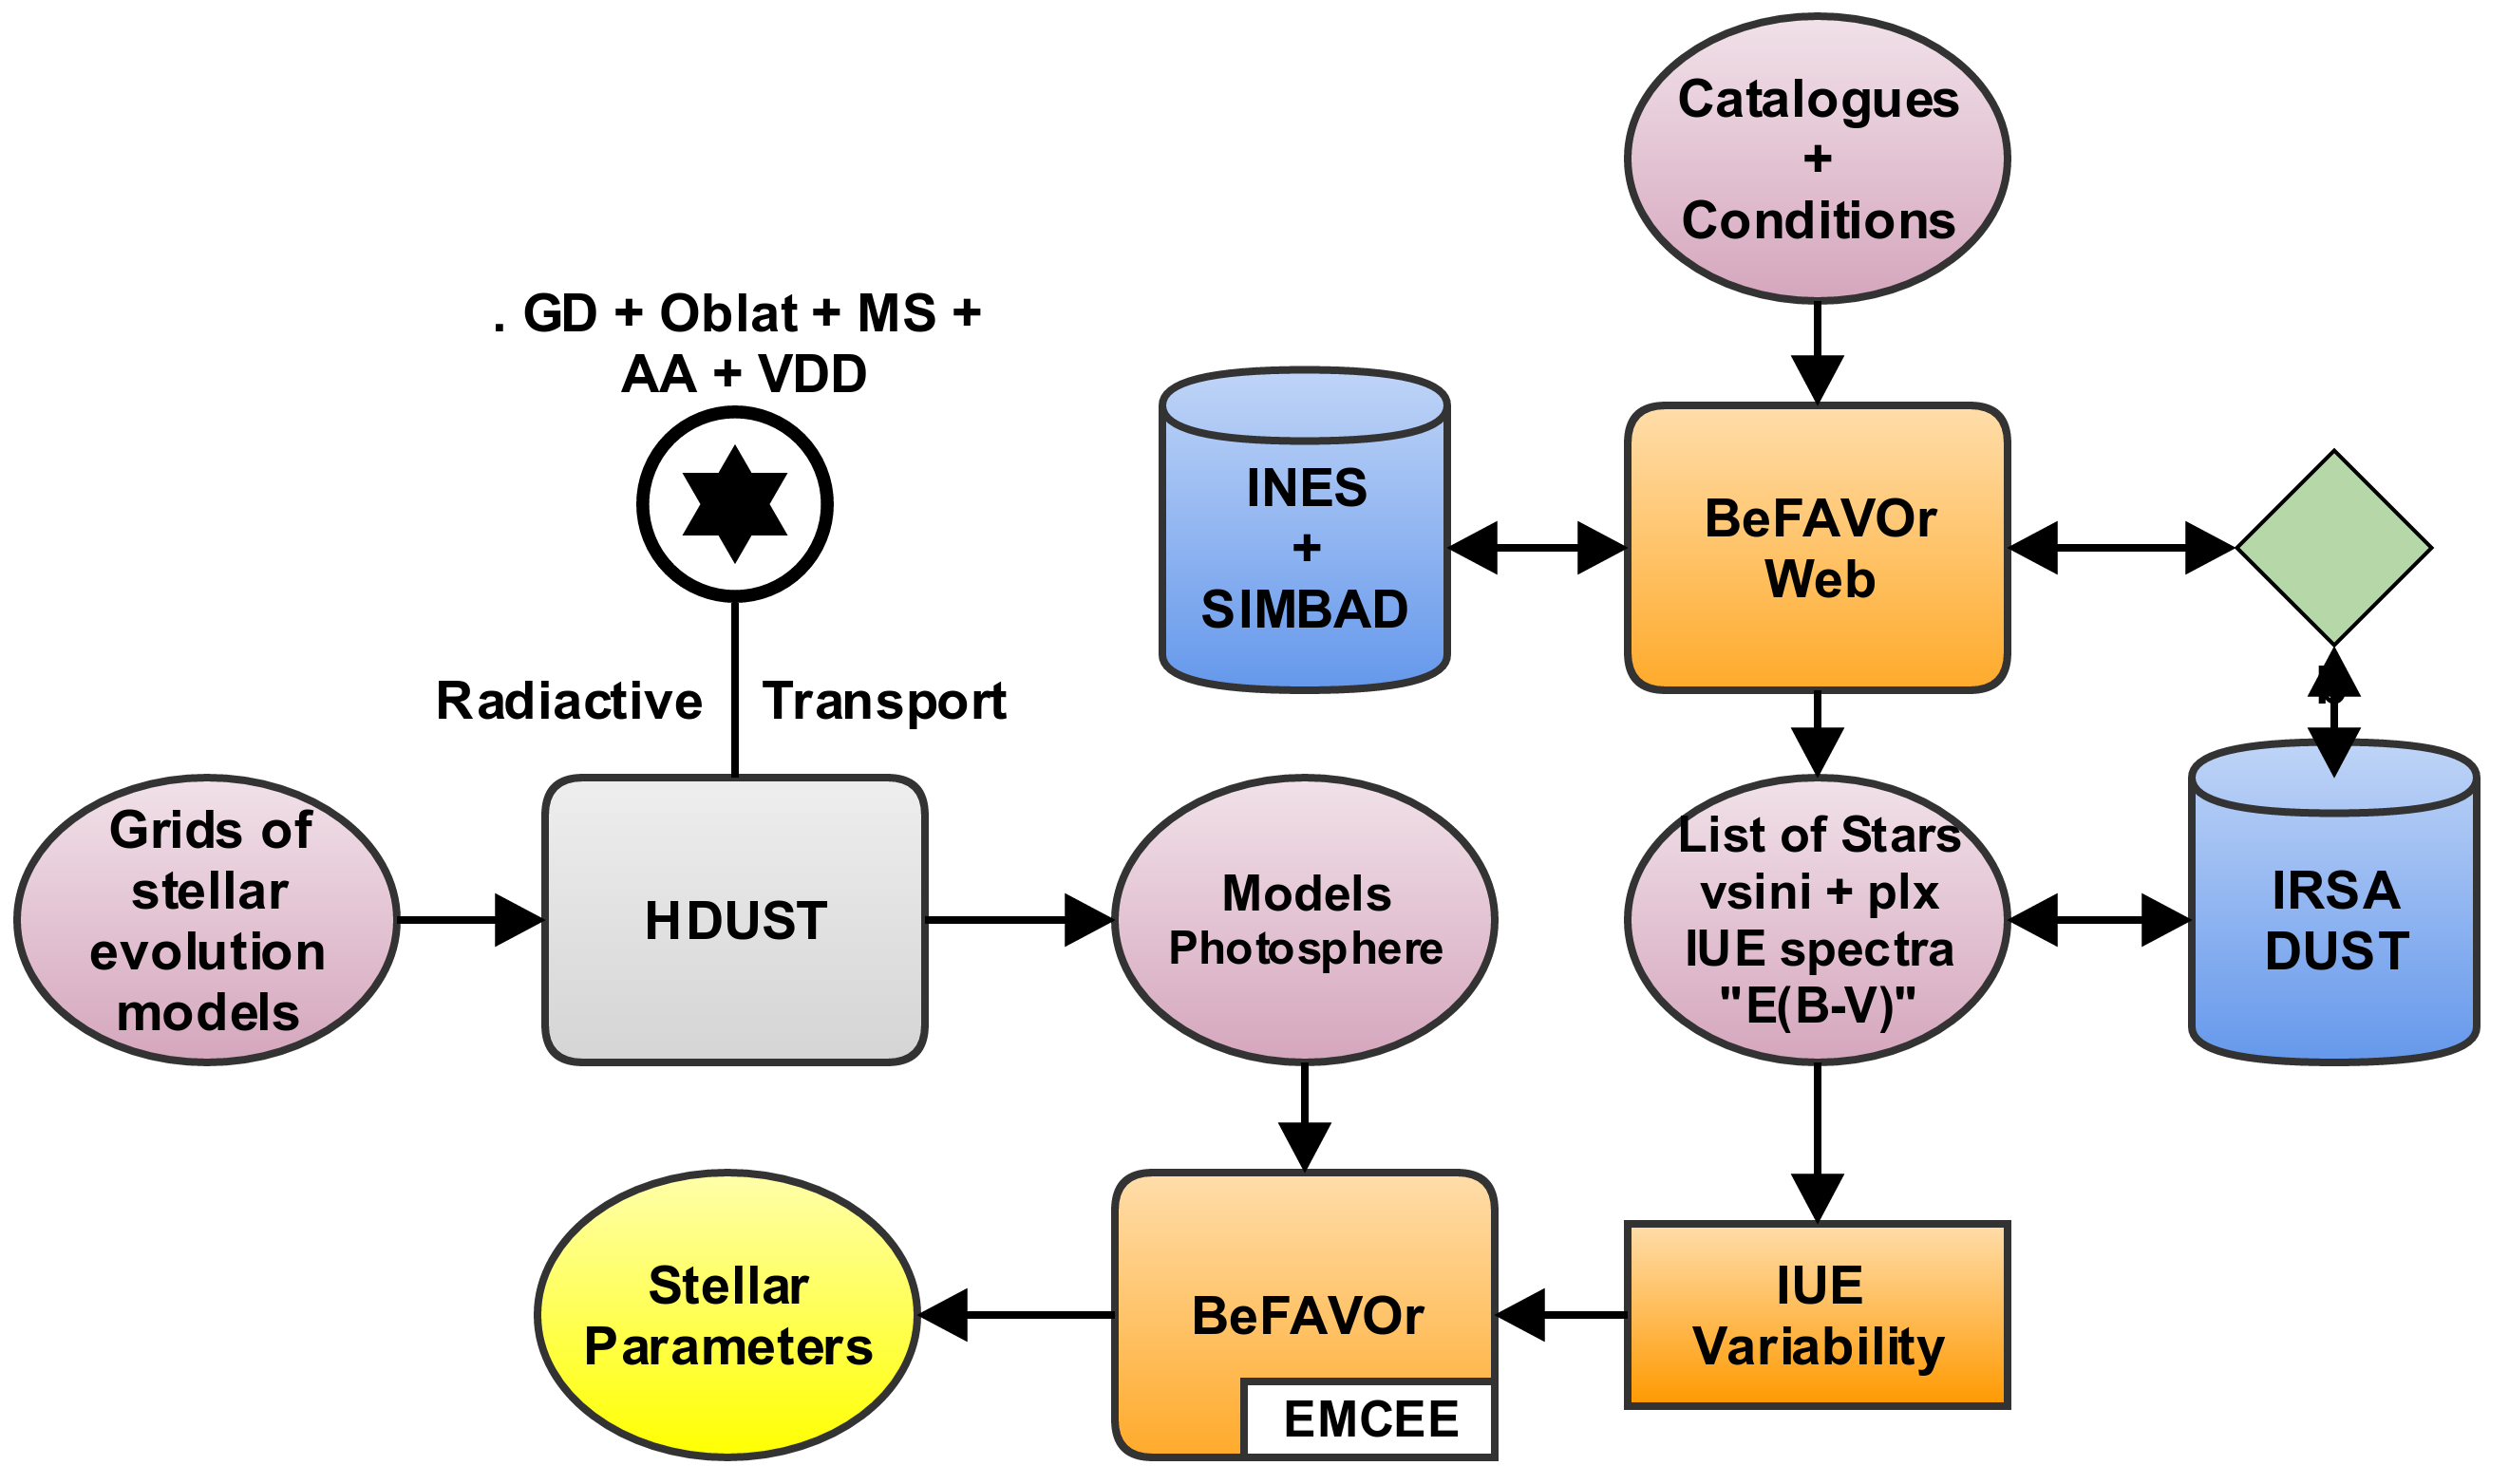
\includegraphics[width=0.600\linewidth]{befavor.png}
\caption{Fluxograma simplificado do método desenvolvido.}\label{index:fig1}\end{figure}

Na figura \_fig1, mostramos uma representação simplificada do método que vem sendo desenvolvido. Neste projeto de iniciação, devenvolvemos o bloco \emph{BeFaVOR web} representado na figura. Em resumo, o usuário necessita apenas selecionar catálogos de interesse, bem como os filtros adequados. A partir deste ponto, a rotina verifica se as estrelas selecionadas possuem dados IUE; caso positivo, dados de paralaxe e vsini são lidos e salvos automaticamente do SIMBAD, juntamente com os espectros do IUE (salvos da plataforma INES). Uma implementação adicional é a verificação da existência de uma região espectral que pode ser utilizada para se determinar o avermelhamento devido ao meio interestelar. Caso ela não exista, a rotina lê e salva uma estimativa do \emph{web service} IRSA. Por fim, o usuário obtêm uma lista de estrelas, com seus respectivos dados de paralaxe, vsini, E(B-V) e incertezas. Estes dados são utilizados na rotina BeFaVOR de determinação dos parâmetros estelares, que está sendo desenvolvida pelo doutorando Bruno C. Mota.


\chapter{Anexos}
\label{index:anexos}

\section{Anexo 1: Rotina BeFaVOr\_web}
\label{index:anexo-1-rotina-befavor-web}
\begin{Verbatim}[commandchars=\\\{\}]
\PYG{c}{\PYGZsh{} 1) Esta rotina deve ser rodada em ipython3}

\PYG{c}{\PYGZsh{} ==============================================================================}
\PYG{c}{\PYGZsh{} Importing modules}
\PYG{k+kn}{import} \PYG{n+nn}{numpy} \PYG{k+kn}{as} \PYG{n+nn}{np}
\PYG{k+kn}{from} \PYG{n+nn}{urllib.request} \PYG{k+kn}{import} \PYG{n}{urlopen}
\PYG{k+kn}{from} \PYG{n+nn}{urllib.error} \PYG{k+kn}{import} \PYG{n}{HTTPError}
\PYG{k+kn}{from} \PYG{n+nn}{bs4} \PYG{k+kn}{import} \PYG{n}{BeautifulSoup}
\PYG{k+kn}{import} \PYG{n+nn}{sys}
\PYG{k+kn}{import} \PYG{n+nn}{re}
\PYG{k+kn}{import} \PYG{n+nn}{datetime}
\PYG{k+kn}{import} \PYG{n+nn}{random}
\PYG{k+kn}{import} \PYG{n+nn}{time}
\PYG{k+kn}{import} \PYG{n+nn}{requests}
\PYG{k+kn}{import} \PYG{n+nn}{math}
\PYG{k+kn}{from} \PYG{n+nn}{selenium} \PYG{k+kn}{import} \PYG{n}{webdriver}
\PYG{k+kn}{from} \PYG{n+nn}{selenium.webdriver.support.ui} \PYG{k+kn}{import} \PYG{n}{Select}
\PYG{k+kn}{import} \PYG{n+nn}{tarfile}
\PYG{k+kn}{from} \PYG{n+nn}{astroquery.simbad} \PYG{k+kn}{import} \PYG{n}{Simbad}
\PYG{k+kn}{import} \PYG{n+nn}{csv}
\PYG{k+kn}{import} \PYG{n+nn}{os}
\PYG{k+kn}{from} \PYG{n+nn}{glob} \PYG{k+kn}{import} \PYG{n}{glob}
\PYG{k+kn}{import} \PYG{n+nn}{pyhdust.phc} \PYG{k+kn}{as} \PYG{n+nn}{phc}
\PYG{k+kn}{import} \PYG{n+nn}{matplotlib.pyplot} \PYG{k+kn}{as} \PYG{n+nn}{plt}
\PYG{k+kn}{from} \PYG{n+nn}{selenium} \PYG{k+kn}{import} \PYG{n}{webdriver}
\PYG{k+kn}{from} \PYG{n+nn}{selenium.webdriver.common.by} \PYG{k+kn}{import} \PYG{n}{By}
\PYG{k+kn}{from} \PYG{n+nn}{selenium.webdriver.support.ui} \PYG{k+kn}{import} \PYG{n}{WebDriverWait}
\PYG{k+kn}{from} \PYG{n+nn}{selenium.webdriver.support} \PYG{k+kn}{import} \PYG{n}{expected\PYGZus{}conditions} \PYG{k}{as} \PYG{n}{EC}


\PYG{c}{\PYGZsh{} ==============================================================================}
\PYG{k}{def} \PYG{n+nf}{show\PYGZus{}page\PYGZus{}code}\PYG{p}{(}\PYG{n}{url}\PYG{p}{)}\PYG{p}{:}
    \PYG{l+s+sd}{\PYGZsq{}\PYGZsq{}\PYGZsq{}}
\PYG{l+s+sd}{    Shows the page code of a certain webpage.}

\PYG{l+s+sd}{    :param url: page url (string)}
\PYG{l+s+sd}{    :return: page code}
\PYG{l+s+sd}{    \PYGZsq{}\PYGZsq{}\PYGZsq{}}

    \PYG{n}{html} \PYG{o}{=} \PYG{n}{urlopen}\PYG{p}{(}\PYG{n}{url}\PYG{p}{)}
    \PYG{n}{bsObj} \PYG{o}{=} \PYG{n}{BeautifulSoup}\PYG{p}{(}\PYG{n}{html}\PYG{o}{.}\PYG{n}{read}\PYG{p}{(}\PYG{p}{)}\PYG{p}{)}
    \PYG{k}{return} \PYG{n}{bsObj}


\PYG{c}{\PYGZsh{} ==============================================================================}
\PYG{k}{def} \PYG{n+nf}{getTitle}\PYG{p}{(}\PYG{n}{url}\PYG{p}{)}\PYG{p}{:}
    \PYG{l+s+sd}{\PYGZsq{}\PYGZsq{}\PYGZsq{}}
\PYG{l+s+sd}{    Gets the title of a certain webpage.}

\PYG{l+s+sd}{    :param url: page url (string)}
\PYG{l+s+sd}{    :return: page title}
\PYG{l+s+sd}{    \PYGZsq{}\PYGZsq{}\PYGZsq{}}

    \PYG{k}{try}\PYG{p}{:}
        \PYG{n}{html} \PYG{o}{=} \PYG{n}{urlopen}\PYG{p}{(}\PYG{n}{url}\PYG{p}{)}
    \PYG{k}{except} \PYG{n}{HTTPError} \PYG{k}{as} \PYG{n}{e}\PYG{p}{:}
        \PYG{k}{print}\PYG{p}{(}\PYG{n}{e}\PYG{p}{)}
        \PYG{k}{return} \PYG{n+nb+bp}{None}
    \PYG{k}{try}\PYG{p}{:}
        \PYG{n}{bsObj} \PYG{o}{=} \PYG{n}{BeautifulSoup}\PYG{p}{(}\PYG{n}{html}\PYG{o}{.}\PYG{n}{read}\PYG{p}{(}\PYG{p}{)}\PYG{p}{)}
        \PYG{n}{title} \PYG{o}{=} \PYG{n}{bsObj}\PYG{o}{.}\PYG{n}{body}\PYG{o}{.}\PYG{n}{h1}
    \PYG{k}{except} \PYG{n+ne}{AttributeError} \PYG{k}{as} \PYG{n}{e}\PYG{p}{:}
        \PYG{k}{return} \PYG{n+nb+bp}{None}
    \PYG{k}{return} \PYG{n}{title}


\PYG{c}{\PYGZsh{} ==============================================================================}
\PYG{k}{def} \PYG{n+nf}{there\PYGZus{}is\PYGZus{}a\PYGZus{}title}\PYG{p}{(}\PYG{n}{url}\PYG{p}{)}\PYG{p}{:}
    \PYG{l+s+sd}{\PYGZsq{}\PYGZsq{}\PYGZsq{}}
\PYG{l+s+sd}{    Prints the title of a certain webpage.}

\PYG{l+s+sd}{    :param url: page url (string)}
\PYG{l+s+sd}{    :return: page title}
\PYG{l+s+sd}{    \PYGZsq{}\PYGZsq{}\PYGZsq{}}

    \PYG{n}{title} \PYG{o}{=} \PYG{n}{getTitle}\PYG{p}{(}\PYG{n}{url}\PYG{p}{)}
    \PYG{k}{if} \PYG{n}{title} \PYG{o+ow}{is} \PYG{n+nb+bp}{None}\PYG{p}{:}
        \PYG{k}{print}\PYG{p}{(}\PYG{l+s}{\PYGZdq{}}\PYG{l+s}{Title could not be found}\PYG{l+s}{\PYGZdq{}}\PYG{p}{)}
    \PYG{k}{else}\PYG{p}{:}
        \PYG{k}{print}\PYG{p}{(}\PYG{n}{title}\PYG{p}{)}
    \PYG{k}{return} \PYG{n}{title}


\PYG{c}{\PYGZsh{} ==============================================================================}
\PYG{k}{def} \PYG{n+nf}{example\PYGZus{}try}\PYG{p}{(}\PYG{p}{)}\PYG{p}{:}

    \PYG{k}{while} \PYG{n+nb+bp}{True}\PYG{p}{:}
        \PYG{k}{try}\PYG{p}{:}
            \PYG{n}{x} \PYG{o}{=} \PYG{n+nb}{int}\PYG{p}{(}\PYG{n+nb}{raw\PYGZus{}input}\PYG{p}{(}\PYG{l+s}{\PYGZdq{}}\PYG{l+s}{Please enter a number: }\PYG{l+s}{\PYGZdq{}}\PYG{p}{)}\PYG{p}{)}
            \PYG{k}{break}
        \PYG{k}{except} \PYG{n+ne}{ValueError}\PYG{p}{:}
            \PYG{k}{print}\PYG{p}{(}\PYG{l+s}{\PYGZdq{}}\PYG{l+s}{Oops!  That was no valid number.  Try again...}\PYG{l+s}{\PYGZdq{}}\PYG{p}{)}
    \PYG{k}{return}


\PYG{c}{\PYGZsh{} ==============================================================================}
\PYG{k}{def} \PYG{n+nf}{get\PYGZus{}attribute}\PYG{p}{(}\PYG{n}{url}\PYG{p}{,} \PYG{n}{atr}\PYG{p}{,} \PYG{n}{typ}\PYG{p}{)}\PYG{p}{:}
    \PYG{l+s+sd}{\PYGZsq{}\PYGZsq{}\PYGZsq{}}
\PYG{l+s+sd}{    Lists all text in a webpage that satisfacts a specified attribute.}

\PYG{l+s+sd}{    :param url: page url (string)}
\PYG{l+s+sd}{    :param atr: attribute (string)}
\PYG{l+s+sd}{    :param typ: tag (string)}
\PYG{l+s+sd}{    :return: text containing specified attribute}
\PYG{l+s+sd}{    \PYGZsq{}\PYGZsq{}\PYGZsq{}}

    \PYG{n}{bsOBJ} \PYG{o}{=} \PYG{n}{show\PYGZus{}page\PYGZus{}code}\PYG{p}{(}\PYG{n}{url}\PYG{p}{)}
    \PYG{n}{namelist} \PYG{o}{=} \PYG{n}{bsOBJ}\PYG{o}{.}\PYG{n}{findAll}\PYG{p}{(}\PYG{n}{typ}\PYG{p}{,} \PYG{p}{\PYGZob{}}\PYG{l+s}{\PYGZdq{}}\PYG{l+s}{class}\PYG{l+s}{\PYGZdq{}}\PYG{p}{:} \PYG{n}{atr}\PYG{p}{\PYGZcb{}}\PYG{p}{)}
    \PYG{n}{names} \PYG{o}{=} \PYG{p}{[}\PYG{p}{]}
    \PYG{k}{for} \PYG{n}{name} \PYG{o+ow}{in} \PYG{n}{namelist}\PYG{p}{:}
        \PYG{n}{nome} \PYG{o}{=} \PYG{n}{name}\PYG{o}{.}\PYG{n}{get\PYGZus{}text}\PYG{p}{(}\PYG{p}{)}
        \PYG{n}{names}\PYG{o}{.}\PYG{n}{append}\PYG{p}{(}\PYG{n}{nome}\PYG{p}{)}

    \PYG{k}{return} \PYG{n}{names}


\PYG{c}{\PYGZsh{} =================================================================================}
\PYG{k}{def} \PYG{n+nf}{find\PYGZus{}regular\PYGZus{}expression}\PYG{p}{(}\PYG{n}{url}\PYG{p}{,} \PYG{n}{typ}\PYG{p}{,} \PYG{n}{atr}\PYG{p}{,} \PYG{n}{expr}\PYG{p}{)}\PYG{p}{:}
    \PYG{l+s+sd}{\PYGZsq{}\PYGZsq{}\PYGZsq{}}
\PYG{l+s+sd}{    Search for a specified expression inside a page code and lists all}
\PYG{l+s+sd}{    its ocurrences.}

\PYG{l+s+sd}{    :param url: page url (string)}
\PYG{l+s+sd}{    :param typ: tag (string)}
\PYG{l+s+sd}{    :param atr: attribute (string)}
\PYG{l+s+sd}{    :param expr: expression (string)}
\PYG{l+s+sd}{    :return: list of occurences}
\PYG{l+s+sd}{    \PYGZsq{}\PYGZsq{}\PYGZsq{}}

    \PYG{n}{html} \PYG{o}{=} \PYG{n}{urlopen}\PYG{p}{(}\PYG{n}{url}\PYG{p}{)}
    \PYG{n}{bsObj} \PYG{o}{=} \PYG{n}{BeautifulSoup}\PYG{p}{(}\PYG{n}{html}\PYG{p}{)}
    \PYG{n}{array} \PYG{o}{=} \PYG{n}{bsObj}\PYG{o}{.}\PYG{n}{findAll}\PYG{p}{(}\PYG{n}{typ}\PYG{p}{,} \PYG{p}{\PYGZob{}}\PYG{n}{atr}\PYG{p}{:} \PYG{n}{re}\PYG{o}{.}\PYG{n}{compile}\PYG{p}{(}\PYG{n}{expr}\PYG{p}{)}\PYG{p}{\PYGZcb{}}\PYG{p}{)}
    \PYG{k}{for} \PYG{n}{lista} \PYG{o+ow}{in} \PYG{n}{array}\PYG{p}{:}
        \PYG{k}{print}\PYG{p}{(}\PYG{n}{lista}\PYG{p}{[}\PYG{l+s}{\PYGZdq{}}\PYG{l+s}{src}\PYG{l+s}{\PYGZdq{}}\PYG{p}{]}\PYG{p}{)}
    \PYG{k}{return} \PYG{n}{lista}


\PYG{c}{\PYGZsh{} ==============================================================================}
\PYG{n}{random}\PYG{o}{.}\PYG{n}{seed}\PYG{p}{(}\PYG{n}{datetime}\PYG{o}{.}\PYG{n}{datetime}\PYG{o}{.}\PYG{n}{now}\PYG{p}{(}\PYG{p}{)}\PYG{p}{)}


\PYG{k}{def} \PYG{n+nf}{getLinks}\PYG{p}{(}\PYG{n}{articleUrl}\PYG{p}{)}\PYG{p}{:}
    \PYG{n}{html} \PYG{o}{=} \PYG{n}{urlopen}\PYG{p}{(}\PYG{l+s}{\PYGZdq{}}\PYG{l+s}{http://en.wikipedia.org}\PYG{l+s}{\PYGZdq{}} \PYG{o}{+} \PYG{n}{articleUrl}\PYG{p}{)}
    \PYG{n}{bsObj} \PYG{o}{=} \PYG{n}{BeautifulSoup}\PYG{p}{(}\PYG{n}{html}\PYG{p}{)}
    \PYG{k}{return} \PYG{n}{bsObj}\PYG{o}{.}\PYG{n}{find}\PYG{p}{(}\PYG{l+s}{\PYGZdq{}}\PYG{l+s}{div}\PYG{l+s}{\PYGZdq{}}\PYG{p}{,} \PYG{p}{\PYGZob{}}\PYG{l+s}{\PYGZdq{}}\PYG{l+s}{id}\PYG{l+s}{\PYGZdq{}}\PYG{p}{:} \PYG{l+s}{\PYGZdq{}}\PYG{l+s}{bodyContent}\PYG{l+s}{\PYGZdq{}}\PYG{p}{\PYGZcb{}}\PYG{p}{)}\PYG{o}{.}\PYGZbs{}
        \PYG{n}{findAll}\PYG{p}{(}\PYG{l+s}{\PYGZdq{}}\PYG{l+s}{a}\PYG{l+s}{\PYGZdq{}}\PYG{p}{,} \PYG{n}{href}\PYG{o}{=}\PYG{n}{re}\PYG{o}{.}\PYG{n}{compile}\PYG{p}{(}\PYG{l+s}{\PYGZdq{}}\PYG{l+s}{\PYGZca{}(/wiki/)((?!:).)*\PYGZdl{}}\PYG{l+s}{\PYGZdq{}}\PYG{p}{)}\PYG{p}{)}


\PYG{c}{\PYGZsh{} ==============================================================================}
\PYG{k}{def} \PYG{n+nf}{get\PYGZus{}Link}\PYG{p}{(}\PYG{n}{articleUrl}\PYG{p}{)}\PYG{p}{:}
    \PYG{n}{links} \PYG{o}{=} \PYG{n}{getLinks}\PYG{p}{(}\PYG{l+s}{\PYGZdq{}}\PYG{l+s}{/wiki/Kevin\PYGZus{}Bacon}\PYG{l+s}{\PYGZdq{}}\PYG{p}{)}
    \PYG{k}{while} \PYG{n+nb}{len}\PYG{p}{(}\PYG{n}{links}\PYG{p}{)} \PYG{o}{\PYGZgt{}} \PYG{l+m+mi}{0}\PYG{p}{:}
        \PYG{n}{newArticle} \PYG{o}{=} \PYG{n}{links}\PYG{p}{[}\PYG{n}{random}\PYG{o}{.}\PYG{n}{randint}\PYG{p}{(}\PYG{l+m+mi}{0}\PYG{p}{,} \PYG{n+nb}{len}\PYG{p}{(}\PYG{n}{links}\PYG{p}{)} \PYG{o}{\PYGZhy{}} \PYG{l+m+mi}{1}\PYG{p}{)}\PYG{p}{]}\PYG{o}{.}\PYG{n}{attrs}\PYG{p}{[}\PYG{l+s}{\PYGZdq{}}\PYG{l+s}{href}\PYG{l+s}{\PYGZdq{}}\PYG{p}{]}
        \PYG{k}{print}\PYG{p}{(}\PYG{n}{newArticle}\PYG{p}{)}
        \PYG{n}{links} \PYG{o}{=} \PYG{n}{getLinks}\PYG{p}{(}\PYG{n}{newArticle}\PYG{p}{)}


\PYG{c}{\PYGZsh{} ==============================================================================}
\PYG{k}{def} \PYG{n+nf}{file\PYGZus{}submission}\PYG{p}{(}\PYG{p}{)}\PYG{p}{:}
    \PYG{n}{files} \PYG{o}{=} \PYG{p}{\PYGZob{}}\PYG{l+s}{\PYGZsq{}}\PYG{l+s}{uploadFile}\PYG{l+s}{\PYGZsq{}}\PYG{p}{:} \PYG{n+nb}{open}\PYG{p}{(}\PYG{l+s}{\PYGZsq{}}\PYG{l+s}{../files/Python\PYGZhy{}logo.png}\PYG{l+s}{\PYGZsq{}}\PYG{p}{,} \PYG{l+s}{\PYGZsq{}}\PYG{l+s}{rb}\PYG{l+s}{\PYGZsq{}}\PYG{p}{)}\PYG{p}{\PYGZcb{}}
    \PYG{n}{r} \PYG{o}{=} \PYG{n}{requests}\PYG{o}{.}\PYG{n}{post}\PYG{p}{(}\PYG{l+s}{\PYGZdq{}}\PYG{l+s}{http://pythonscraping.com/pages/processing2.php}\PYG{l+s}{\PYGZdq{}}\PYG{p}{,}
                      \PYG{n}{files}\PYG{o}{=}\PYG{n}{files}\PYG{p}{)}
    \PYG{k}{print}\PYG{p}{(}\PYG{n}{r}\PYG{o}{.}\PYG{n}{text}\PYG{p}{)}
    \PYG{k}{return}


\PYG{c}{\PYGZsh{} ==============================================================================}
\PYG{k}{def} \PYG{n+nf}{simple\PYGZus{}form}\PYG{p}{(}\PYG{p}{)}\PYG{p}{:}
    \PYG{n}{params} \PYG{o}{=} \PYG{p}{\PYGZob{}}\PYG{l+s}{\PYGZsq{}}\PYG{l+s}{firstname}\PYG{l+s}{\PYGZsq{}}\PYG{p}{:} \PYG{l+s}{\PYGZsq{}}\PYG{l+s}{Ryan}\PYG{l+s}{\PYGZsq{}}\PYG{p}{,} \PYG{l+s}{\PYGZsq{}}\PYG{l+s}{lastname}\PYG{l+s}{\PYGZsq{}}\PYG{p}{:} \PYG{l+s}{\PYGZsq{}}\PYG{l+s}{Mitchell}\PYG{l+s}{\PYGZsq{}}\PYG{p}{\PYGZcb{}}
    \PYG{n}{r} \PYG{o}{=} \PYG{n}{requests}\PYG{o}{.}\PYG{n}{post}\PYG{p}{(}\PYG{l+s}{\PYGZdq{}}\PYG{l+s}{http://pythonscraping.com/files/processing.php}\PYG{l+s}{\PYGZdq{}}\PYG{p}{,}
                      \PYG{n}{data}\PYG{o}{=}\PYG{n}{params}\PYG{p}{)}
    \PYG{k}{print}\PYG{p}{(}\PYG{n}{r}\PYG{o}{.}\PYG{n}{text}\PYG{p}{)}
    \PYG{k}{return}


\PYG{c}{\PYGZsh{} ==============================================================================}
\PYG{k}{def} \PYG{n+nf}{file\PYGZus{}submission2}\PYG{p}{(}\PYG{p}{)}\PYG{p}{:}
    \PYG{n}{files} \PYG{o}{=} \PYG{p}{\PYGZob{}}\PYG{l+s}{\PYGZsq{}}\PYG{l+s}{uploadFile}\PYG{l+s}{\PYGZsq{}}\PYG{p}{:} \PYG{n+nb}{open}\PYG{p}{(}\PYG{l+s}{\PYGZsq{}}\PYG{l+s}{../files/python.png}\PYG{l+s}{\PYGZsq{}}\PYG{p}{,} \PYG{l+s}{\PYGZsq{}}\PYG{l+s}{rb}\PYG{l+s}{\PYGZsq{}}\PYG{p}{)}\PYG{p}{\PYGZcb{}}
    \PYG{n}{r} \PYG{o}{=} \PYG{n}{requests}\PYG{o}{.}\PYG{n}{post}\PYG{p}{(}\PYG{l+s}{\PYGZdq{}}\PYG{l+s}{http://pythonscraping.com/pages/processing2.php}\PYG{l+s}{\PYGZdq{}}\PYG{p}{,}
                      \PYG{n}{files}\PYG{o}{=}\PYG{n}{files}\PYG{p}{)}
    \PYG{k}{print}\PYG{p}{(}\PYG{n}{r}\PYG{o}{.}\PYG{n}{text}\PYG{p}{)}

    \PYG{k}{return}


\PYG{c}{\PYGZsh{} ==============================================================================}
\PYG{k}{def} \PYG{n+nf}{iue\PYGZus{}submission}\PYG{p}{(}\PYG{n}{star\PYGZus{}name}\PYG{p}{)}\PYG{p}{:}
    \PYG{l+s+sd}{\PYGZsq{}\PYGZsq{}\PYGZsq{}}
\PYG{l+s+sd}{    Search in the IUE database for a certain star name.}
\PYG{l+s+sd}{    }
\PYG{l+s+sd}{    :param star\PYGZus{}name: name of the star (string)}
\PYG{l+s+sd}{    :return: request of star name in IUE page}
\PYG{l+s+sd}{    \PYGZsq{}\PYGZsq{}\PYGZsq{}}

    \PYG{n}{ines\PYGZus{}site} \PYG{o}{=} \PYG{l+s}{\PYGZdq{}}\PYG{l+s}{http://sdc.cab.inta\PYGZhy{}csic.es/cgi\PYGZhy{}ines/IUEdbsMY}\PYG{l+s}{\PYGZdq{}}
    \PYG{n}{params} \PYG{o}{=} \PYG{p}{\PYGZob{}}\PYG{l+s}{\PYGZsq{}}\PYG{l+s}{object}\PYG{l+s}{\PYGZsq{}}\PYG{p}{:} \PYG{n}{star\PYGZus{}name}\PYG{p}{\PYGZcb{}}
    \PYG{n}{r} \PYG{o}{=} \PYG{n}{requests}\PYG{o}{.}\PYG{n}{post}\PYG{p}{(}\PYG{n}{ines\PYGZus{}site}\PYG{p}{,} \PYG{n}{data}\PYG{o}{=}\PYG{n}{params}\PYG{p}{)}
    \PYG{k}{print}\PYG{p}{(}\PYG{n}{r}\PYG{o}{.}\PYG{n}{text}\PYG{p}{)}

    \PYG{k}{return} \PYG{n}{r}


\PYG{c}{\PYGZsh{} ==============================================================================}
\PYG{k}{def} \PYG{n+nf}{read\PYGZus{}txt}\PYG{p}{(}\PYG{n}{list\PYGZus{}name}\PYG{p}{,} \PYG{n}{folder}\PYG{p}{)}\PYG{p}{:}
    \PYG{l+s+sd}{\PYGZsq{}\PYGZsq{}\PYGZsq{}}
\PYG{l+s+sd}{    Read a given list of star names.}
\PYG{l+s+sd}{    }
\PYG{l+s+sd}{    :param list\PYGZus{}name: name o txt file containing the list (string)}
\PYG{l+s+sd}{    :param folder: list\PYGZsq{}s folder (string)}
\PYG{l+s+sd}{    :return: column of the list read}
\PYG{l+s+sd}{    \PYGZsq{}\PYGZsq{}\PYGZsq{}}

    \PYG{n}{list\PYGZus{}name} \PYG{o}{=} \PYG{n}{folder} \PYG{o}{+} \PYG{n}{list\PYGZus{}name}

    \PYG{n}{cols} \PYG{o}{=} \PYG{n}{np}\PYG{o}{.}\PYG{n}{genfromtxt}\PYG{p}{(}\PYG{n}{list\PYGZus{}name}\PYG{p}{,} \PYG{n}{unpack}\PYG{o}{=}\PYG{n+nb+bp}{True}\PYG{p}{,} \PYG{n}{comments}\PYG{o}{=}\PYG{l+s}{\PYGZsq{}}\PYG{l+s}{\PYGZsh{}}\PYG{l+s}{\PYGZsq{}}\PYG{p}{,}
                         \PYG{n}{delimiter}\PYG{o}{=}\PYG{l+s}{\PYGZsq{}}\PYG{l+s+se}{\PYGZbs{}t}\PYG{l+s}{\PYGZsq{}}\PYG{p}{)}

    \PYG{k}{return} \PYG{n}{cols}


\PYG{c}{\PYGZsh{} ==============================================================================}
\PYG{k}{def} \PYG{n+nf}{untar}\PYG{p}{(}\PYG{n}{fname}\PYG{p}{)}\PYG{p}{:}
    \PYG{l+s+sd}{\PYGZsq{}\PYGZsq{}\PYGZsq{}}
\PYG{l+s+sd}{    Decompact a tar file.}
\PYG{l+s+sd}{    }
\PYG{l+s+sd}{    :param fname: name o file to be decompacted (string)}
\PYG{l+s+sd}{    :return: decompacted file}
\PYG{l+s+sd}{    \PYGZsq{}\PYGZsq{}\PYGZsq{}}

    \PYG{k}{if} \PYG{p}{(}\PYG{n}{fname}\PYG{o}{.}\PYG{n}{endswith}\PYG{p}{(}\PYG{l+s}{\PYGZdq{}}\PYG{l+s}{tar.gz}\PYG{l+s}{\PYGZdq{}}\PYG{p}{)}\PYG{p}{)}\PYG{p}{:}
        \PYG{n}{tar} \PYG{o}{=} \PYG{n}{tarfile}\PYG{o}{.}\PYG{n}{open}\PYG{p}{(}\PYG{n}{fname}\PYG{p}{)}
        \PYG{n}{tar}\PYG{o}{.}\PYG{n}{extractall}\PYG{p}{(}\PYG{p}{)}
        \PYG{n}{tar}\PYG{o}{.}\PYG{n}{close}\PYG{p}{(}\PYG{p}{)}
        \PYG{k}{print}\PYG{p}{(}\PYG{l+s}{\PYGZdq{}}\PYG{l+s}{Extracted in Current Directory}\PYG{l+s}{\PYGZdq{}}\PYG{p}{)}
    \PYG{k}{else}\PYG{p}{:}
        \PYG{k}{print}\PYG{p}{(}\PYG{l+s}{\PYGZdq{}}\PYG{l+s}{Not a tar.gz file: }\PYG{l+s}{\PYGZsq{}}\PYG{l+s+si}{\PYGZpc{}s}\PYG{l+s}{ }\PYG{l+s}{\PYGZsq{}}\PYG{l+s}{\PYGZdq{}} \PYG{o}{\PYGZpc{}} \PYG{n}{sys}\PYG{o}{.}\PYG{n}{argv}\PYG{p}{[}\PYG{l+m+mi}{0}\PYG{p}{]}\PYG{p}{)}


\PYG{c}{\PYGZsh{} ==============================================================================}
\PYG{k}{def} \PYG{n+nf}{create\PYGZus{}list\PYGZus{}files}\PYG{p}{(}\PYG{n}{list\PYGZus{}name}\PYG{p}{,} \PYG{n}{folder}\PYG{p}{,} \PYG{n}{folder\PYGZus{}table}\PYG{p}{)}\PYG{p}{:}
    \PYG{l+s+sd}{\PYGZsq{}\PYGZsq{}\PYGZsq{}}
\PYG{l+s+sd}{    Creates a list of the files inside a given folder.}

\PYG{l+s+sd}{    :param list\PYGZus{}name: list\PYGZsq{}s name (string)}
\PYG{l+s+sd}{    :param folder: files\PYGZsq{} folder (string)}
\PYG{l+s+sd}{    :return: creates a txt file, with the files\PYGZsq{} paths}
\PYG{l+s+sd}{    \PYGZsq{}\PYGZsq{}\PYGZsq{}}

    \PYG{n}{a} \PYG{o}{=} \PYG{n+nb}{open}\PYG{p}{(}\PYG{n}{folder\PYGZus{}table} \PYG{o}{+} \PYG{n}{list\PYGZus{}name} \PYG{o}{+} \PYG{l+s}{\PYGZdq{}}\PYG{l+s}{.txt}\PYG{l+s}{\PYGZdq{}}\PYG{p}{,} \PYG{l+s}{\PYGZdq{}}\PYG{l+s}{w}\PYG{l+s}{\PYGZdq{}}\PYG{p}{)}
    \PYG{k}{for} \PYG{n}{path}\PYG{p}{,} \PYG{n}{subdirs}\PYG{p}{,} \PYG{n}{files} \PYG{o+ow}{in} \PYG{n}{os}\PYG{o}{.}\PYG{n}{walk}\PYG{p}{(}\PYG{n}{folder}\PYG{p}{)}\PYG{p}{:}
        \PYG{k}{for} \PYG{n}{filename} \PYG{o+ow}{in} \PYG{n}{files}\PYG{p}{:}
            \PYG{n}{f} \PYG{o}{=} \PYG{n}{os}\PYG{o}{.}\PYG{n}{path}\PYG{o}{.}\PYG{n}{join}\PYG{p}{(}\PYG{n}{path}\PYG{p}{,} \PYG{n}{filename}\PYG{p}{)}
            \PYG{n}{a}\PYG{o}{.}\PYG{n}{write}\PYG{p}{(}\PYG{n+nb}{str}\PYG{p}{(}\PYG{n}{f}\PYG{p}{)} \PYG{o}{+} \PYG{n}{os}\PYG{o}{.}\PYG{n}{linesep}\PYG{p}{)}
    \PYG{k}{return}


\PYG{c}{\PYGZsh{} ==============================================================================}
\PYG{k}{def} \PYG{n+nf}{create\PYGZus{}txt\PYGZus{}file}\PYG{p}{(}\PYG{n}{data\PYGZus{}list}\PYG{p}{,} \PYG{n}{file\PYGZus{}name}\PYG{p}{)}\PYG{p}{:}
    \PYG{l+s+sd}{\PYGZsq{}\PYGZsq{}\PYGZsq{}}
\PYG{l+s+sd}{    Create a txt file.}

\PYG{l+s+sd}{    :param data\PYGZus{}list: list of data to be saved (array)}
\PYG{l+s+sd}{    :param file\PYGZus{}name: txt file\PYGZsq{}s name (string)}
\PYG{l+s+sd}{    :return: txt file}
\PYG{l+s+sd}{    \PYGZsq{}\PYGZsq{}\PYGZsq{}}

    \PYG{k}{with} \PYG{n+nb}{open}\PYG{p}{(}\PYG{n}{file\PYGZus{}name}\PYG{p}{,} \PYG{l+s}{\PYGZsq{}}\PYG{l+s}{w}\PYG{l+s}{\PYGZsq{}}\PYG{p}{)} \PYG{k}{as} \PYG{n}{f}\PYG{p}{:}
        \PYG{n}{writer} \PYG{o}{=} \PYG{n}{csv}\PYG{o}{.}\PYG{n}{writer}\PYG{p}{(}\PYG{n}{f}\PYG{p}{,} \PYG{n}{delimiter}\PYG{o}{=}\PYG{l+s}{\PYGZsq{}}\PYG{l+s+se}{\PYGZbs{}t}\PYG{l+s}{\PYGZsq{}}\PYG{p}{)}
        \PYG{n}{writer}\PYG{o}{.}\PYG{n}{writerows}\PYG{p}{(}\PYG{n+nb}{zip}\PYG{p}{(}\PYG{n}{data\PYGZus{}list}\PYG{p}{)}\PYG{p}{)}
    \PYG{k}{return}


\PYG{c}{\PYGZsh{} ==============================================================================}
\PYG{k}{def} \PYG{n+nf}{read\PYGZus{}simbad\PYGZus{}data}\PYG{p}{(}\PYG{n}{star\PYGZus{}name}\PYG{p}{)}\PYG{p}{:}
    \PYG{l+s+sd}{\PYGZsq{}\PYGZsq{}\PYGZsq{}}
\PYG{l+s+sd}{    Query SIMBAD for a given star parallax, vsini, bump and references.}

\PYG{l+s+sd}{    :param star\PYGZus{}name: star\PYGZsq{}s name (string)}
\PYG{l+s+sd}{    :return: txt file with star\PYGZsq{}s parallax, vsini, bump, the respective}
\PYG{l+s+sd}{    errors and references for vsini and E(B\PYGZhy{}V)}
\PYG{l+s+sd}{    \PYGZsq{}\PYGZsq{}\PYGZsq{}}

    \PYG{n}{customSimbad} \PYG{o}{=} \PYG{n}{Simbad}\PYG{p}{(}\PYG{p}{)}
    \PYG{c}{\PYGZsh{} customSimbad.list\PYGZus{}votable\PYGZus{}fields() \PYGZsh{}  to list all avaiable fields}
    \PYG{n}{customSimbad}\PYG{o}{.}\PYG{n}{get\PYGZus{}votable\PYGZus{}fields}\PYG{p}{(}\PYG{p}{)}
    \PYG{n}{customSimbad}\PYG{o}{.}\PYG{n}{add\PYGZus{}votable\PYGZus{}fields}\PYG{p}{(}\PYG{l+s}{\PYGZsq{}}\PYG{l+s}{plx}\PYG{l+s}{\PYGZsq{}}\PYG{p}{,} \PYG{l+s}{\PYGZsq{}}\PYG{l+s}{plx\PYGZus{}error}\PYG{l+s}{\PYGZsq{}}\PYG{p}{,} \PYG{l+s}{\PYGZsq{}}\PYG{l+s}{rot}\PYG{l+s}{\PYGZsq{}}\PYG{p}{)}
    \PYG{n}{customSimbad}\PYG{o}{.}\PYG{n}{get\PYGZus{}votable\PYGZus{}fields}\PYG{p}{(}\PYG{p}{)}
    \PYG{n}{result\PYGZus{}table} \PYG{o}{=} \PYG{n}{customSimbad}\PYG{o}{.}\PYG{n}{query\PYGZus{}object}\PYG{p}{(}\PYG{n}{star\PYGZus{}name}\PYG{p}{)}
    \PYG{c}{\PYGZsh{} star = result\PYGZus{}table[\PYGZsq{}MAIN\PYGZus{}ID\PYGZsq{}]}
    \PYG{n}{star} \PYG{o}{=} \PYG{n}{np}\PYG{o}{.}\PYG{n}{copy}\PYG{p}{(}\PYG{n}{star\PYGZus{}name}\PYG{p}{)}
    \PYG{n}{plx} \PYG{o}{=} \PYG{n}{result\PYGZus{}table}\PYG{p}{[}\PYG{l+s}{\PYGZsq{}}\PYG{l+s}{PLX\PYGZus{}VALUE}\PYG{l+s}{\PYGZsq{}}\PYG{p}{]}\PYG{p}{[}\PYG{l+m+mi}{0}\PYG{p}{]}
    \PYG{n}{plx\PYGZus{}error} \PYG{o}{=} \PYG{n}{result\PYGZus{}table}\PYG{p}{[}\PYG{l+s}{\PYGZsq{}}\PYG{l+s}{PLX\PYGZus{}ERROR}\PYG{l+s}{\PYGZsq{}}\PYG{p}{]}\PYG{p}{[}\PYG{l+m+mi}{0}\PYG{p}{]}
    \PYG{n}{vsini} \PYG{o}{=} \PYG{n}{result\PYGZus{}table}\PYG{p}{[}\PYG{l+s}{\PYGZsq{}}\PYG{l+s}{ROT\PYGZus{}Vsini}\PYG{l+s}{\PYGZsq{}}\PYG{p}{]}\PYG{p}{[}\PYG{l+m+mi}{0}\PYG{p}{]}
    \PYG{n}{vsini\PYGZus{}err} \PYG{o}{=} \PYG{n}{result\PYGZus{}table}\PYG{p}{[}\PYG{l+s}{\PYGZsq{}}\PYG{l+s}{ROT\PYGZus{}err}\PYG{l+s}{\PYGZsq{}}\PYG{p}{]}\PYG{o}{.}\PYG{n}{item}\PYG{p}{(}\PYG{p}{)}
    \PYG{n}{rot\PYGZus{}bibcode} \PYG{o}{=} \PYG{n}{result\PYGZus{}table}\PYG{p}{[}\PYG{l+s}{\PYGZsq{}}\PYG{l+s}{ROT\PYGZus{}bibcode}\PYG{l+s}{\PYGZsq{}}\PYG{p}{]}
    \PYG{n}{bump} \PYG{o}{=} \PYG{n+nb+bp}{True}
    \PYG{n}{ebmv\PYGZus{}ref} \PYG{o}{=} \PYG{l+m+mf}{0.0}

    \PYG{k}{return} \PYG{n}{star}\PYG{o}{.}\PYG{n}{item}\PYG{p}{(}\PYG{p}{)}\PYG{p}{,} \PYG{n}{plx}\PYG{p}{,} \PYG{n}{plx\PYGZus{}error}\PYG{p}{,} \PYG{n}{vsini}\PYG{p}{,} \PYG{n}{vsini\PYGZus{}err}\PYG{p}{,} \PYG{n}{bump}\PYG{p}{,}\PYGZbs{}
        \PYG{n}{rot\PYGZus{}bibcode}\PYG{o}{.}\PYG{n}{item}\PYG{p}{(}\PYG{p}{)}\PYG{p}{,} \PYG{n}{ebmv\PYGZus{}ref}


\PYG{c}{\PYGZsh{} ==============================================================================}
\PYG{k}{def} \PYG{n+nf}{read\PYGZus{}simbad\PYGZus{}coodr}\PYG{p}{(}\PYG{n}{star\PYGZus{}name}\PYG{p}{)}\PYG{p}{:}
    \PYG{l+s+sd}{\PYGZsq{}\PYGZsq{}\PYGZsq{}}
\PYG{l+s+sd}{    Query SIMBAD for the coordinates of a given star.}

\PYG{l+s+sd}{    :param star\PYGZus{}name: star\PYGZsq{}s name (string)}
\PYG{l+s+sd}{    :return: right ascencion and declination coordinates}
\PYG{l+s+sd}{    \PYGZsq{}\PYGZsq{}\PYGZsq{}}

    \PYG{n}{customSimbad} \PYG{o}{=} \PYG{n}{Simbad}\PYG{p}{(}\PYG{p}{)}
    \PYG{n}{customSimbad}\PYG{o}{.}\PYG{n}{get\PYGZus{}votable\PYGZus{}fields}\PYG{p}{(}\PYG{p}{)}
    \PYG{n}{result\PYGZus{}table} \PYG{o}{=} \PYG{n}{customSimbad}\PYG{o}{.}\PYG{n}{query\PYGZus{}object}\PYG{p}{(}\PYG{n}{star\PYGZus{}name}\PYG{p}{)}

    \PYG{n}{ra} \PYG{o}{=} \PYG{n}{result\PYGZus{}table}\PYG{p}{[}\PYG{l+s}{\PYGZsq{}}\PYG{l+s}{RA}\PYG{l+s}{\PYGZsq{}}\PYG{p}{]}\PYG{p}{[}\PYG{l+m+mi}{0}\PYG{p}{]}
    \PYG{n}{dec} \PYG{o}{=} \PYG{n}{result\PYGZus{}table}\PYG{p}{[}\PYG{l+s}{\PYGZsq{}}\PYG{l+s}{DEC}\PYG{l+s}{\PYGZsq{}}\PYG{p}{]}\PYG{p}{[}\PYG{l+m+mi}{0}\PYG{p}{]}

    \PYG{k}{return} \PYG{n}{ra}\PYG{p}{,} \PYG{n}{dec}


\PYG{c}{\PYGZsh{} ==============================================================================}
\PYG{k}{def} \PYG{n+nf}{unzip}\PYG{p}{(}\PYG{n}{zip\PYGZus{}file}\PYG{p}{,} \PYG{n}{outdir}\PYG{p}{)}\PYG{p}{:}
    \PYG{l+s+sd}{\PYGZsq{}\PYGZsq{}\PYGZsq{}}
\PYG{l+s+sd}{    Unzip a given file into the specified output directory.}

\PYG{l+s+sd}{    :param zip\PYGZus{}file: name of file to be unziped (string)}
\PYG{l+s+sd}{    :param outdir: directory of the file (string)}
\PYG{l+s+sd}{    :return: unziped file}
\PYG{l+s+sd}{    \PYGZsq{}\PYGZsq{}\PYGZsq{}}

    \PYG{k+kn}{import} \PYG{n+nn}{zipfile}
    \PYG{n}{zf} \PYG{o}{=} \PYG{n}{zipfile}\PYG{o}{.}\PYG{n}{ZipFile}\PYG{p}{(}\PYG{n}{zip\PYGZus{}file}\PYG{p}{,} \PYG{l+s}{\PYGZdq{}}\PYG{l+s}{r}\PYG{l+s}{\PYGZdq{}}\PYG{p}{)}
    \PYG{n}{zf}\PYG{o}{.}\PYG{n}{extractall}\PYG{p}{(}\PYG{n}{outdir}\PYG{p}{)}
    \PYG{k}{return}


\PYG{c}{\PYGZsh{} ==============================================================================}
\PYG{k}{def} \PYG{n+nf}{plot\PYGZus{}gal}\PYG{p}{(}\PYG{n}{ra\PYGZus{}val}\PYG{p}{,} \PYG{n}{dec\PYGZus{}val}\PYG{p}{,} \PYG{n}{folder\PYGZus{}fig}\PYG{p}{)}\PYG{p}{:}
    \PYG{l+s+sd}{\PYGZdq{}\PYGZdq{}\PYGZdq{}}
\PYG{l+s+sd}{    Plot in \PYGZdq{}Galatic Coordinates\PYGZdq{} (i.e., Mollweide projection).}

\PYG{l+s+sd}{    :param ra\PYGZus{}val: right ascencion in RADIANS (float)}
\PYG{l+s+sd}{    :param dec\PYGZus{}val: declination in RADIANS (float)}
\PYG{l+s+sd}{    :param folder\PYGZus{}fig: name of the folder for the figure (string)}
\PYG{l+s+sd}{    :return: saved images}
\PYG{l+s+sd}{    \PYGZdq{}\PYGZdq{}\PYGZdq{}}

    \PYG{n}{fig} \PYG{o}{=} \PYG{n}{plt}\PYG{o}{.}\PYG{n}{figure}\PYG{p}{(}\PYG{p}{)}
    \PYG{n}{ax} \PYG{o}{=} \PYG{n}{fig}\PYG{o}{.}\PYG{n}{add\PYGZus{}subplot}\PYG{p}{(}\PYG{l+m+mi}{111}\PYG{p}{,} \PYG{n}{projection}\PYG{o}{=}\PYG{l+s}{\PYGZdq{}}\PYG{l+s}{mollweide}\PYG{l+s}{\PYGZdq{}}\PYG{p}{)}
    \PYG{n}{ax}\PYG{o}{.}\PYG{n}{set\PYGZus{}xticklabels}\PYG{p}{(}\PYG{p}{[}\PYG{l+s}{\PYGZsq{}}\PYG{l+s}{14h}\PYG{l+s}{\PYGZsq{}}\PYG{p}{,} \PYG{l+s}{\PYGZsq{}}\PYG{l+s}{16h}\PYG{l+s}{\PYGZsq{}}\PYG{p}{,} \PYG{l+s}{\PYGZsq{}}\PYG{l+s}{18h}\PYG{l+s}{\PYGZsq{}}\PYG{p}{,} \PYG{l+s}{\PYGZsq{}}\PYG{l+s}{20h}\PYG{l+s}{\PYGZsq{}}\PYG{p}{,} \PYG{l+s}{\PYGZsq{}}\PYG{l+s}{22h}\PYG{l+s}{\PYGZsq{}}\PYG{p}{,} \PYG{l+s}{\PYGZsq{}}\PYG{l+s}{0h}\PYG{l+s}{\PYGZsq{}}\PYG{p}{,} \PYG{l+s}{\PYGZsq{}}\PYG{l+s}{2h}\PYG{l+s}{\PYGZsq{}}\PYG{p}{,} \PYG{l+s}{\PYGZsq{}}\PYG{l+s}{4h}\PYG{l+s}{\PYGZsq{}}\PYG{p}{,}
                        \PYG{l+s}{\PYGZsq{}}\PYG{l+s}{6h}\PYG{l+s}{\PYGZsq{}}\PYG{p}{,} \PYG{l+s}{\PYGZsq{}}\PYG{l+s}{8h}\PYG{l+s}{\PYGZsq{}}\PYG{p}{,} \PYG{l+s}{\PYGZsq{}}\PYG{l+s}{10h}\PYG{l+s}{\PYGZsq{}}\PYG{p}{]}\PYG{p}{)}

    \PYG{k}{for} \PYG{n}{i} \PYG{o+ow}{in} \PYG{n+nb}{range}\PYG{p}{(}\PYG{n+nb}{len}\PYG{p}{(}\PYG{n}{ra\PYGZus{}val}\PYG{p}{)}\PYG{p}{)}\PYG{p}{:}
        \PYG{n}{dec} \PYG{o}{=} \PYG{n}{dec\PYGZus{}val}\PYG{p}{[}\PYG{n}{i}\PYG{p}{]}\PYG{o}{.}\PYG{n}{replace}\PYG{p}{(}\PYG{l+s}{\PYGZsq{}}\PYG{l+s}{ }\PYG{l+s}{\PYGZsq{}}\PYG{p}{,} \PYG{l+s}{\PYGZsq{}}\PYG{l+s}{:}\PYG{l+s}{\PYGZsq{}}\PYG{p}{)}
        \PYG{n}{ra} \PYG{o}{=} \PYG{n}{ra\PYGZus{}val}\PYG{p}{[}\PYG{n}{i}\PYG{p}{]}\PYG{o}{.}\PYG{n}{replace}\PYG{p}{(}\PYG{l+s}{\PYGZsq{}}\PYG{l+s}{ }\PYG{l+s}{\PYGZsq{}}\PYG{p}{,} \PYG{l+s}{\PYGZsq{}}\PYG{l+s}{:}\PYG{l+s}{\PYGZsq{}}\PYG{p}{)}

        \PYG{c}{\PYGZsh{} list of floats (degrees fraction)}
        \PYG{n}{dec} \PYG{o}{=} \PYG{p}{[}\PYG{n}{phc}\PYG{o}{.}\PYG{n}{dec2degf}\PYG{p}{(}\PYG{n}{dec}\PYG{p}{)}\PYG{p}{]}
        \PYG{n}{ra} \PYG{o}{=} \PYG{p}{[}\PYG{n}{phc}\PYG{o}{.}\PYG{n}{ra2degf}\PYG{p}{(}\PYG{n}{ra}\PYG{p}{)}\PYG{p}{]}

        \PYG{c}{\PYGZsh{} arrays of floats (radians)}
        \PYG{n}{dec} \PYG{o}{=} \PYG{n}{np}\PYG{o}{.}\PYG{n}{array}\PYG{p}{(}\PYG{n}{dec}\PYG{p}{)} \PYG{o}{*} \PYG{n}{np}\PYG{o}{.}\PYG{n}{pi} \PYG{o}{/} \PYG{l+m+mi}{180}
        \PYG{n}{ra} \PYG{o}{=} \PYG{n}{np}\PYG{o}{.}\PYG{n}{array}\PYG{p}{(}\PYG{n}{ra}\PYG{p}{)} \PYG{o}{*} \PYG{n}{np}\PYG{o}{.}\PYG{n}{pi} \PYG{o}{/} \PYG{l+m+mi}{180}

        \PYG{n}{ax}\PYG{o}{.}\PYG{n}{scatter}\PYG{p}{(}\PYG{n}{ra}\PYG{p}{,} \PYG{n}{dec}\PYG{p}{)}
    \PYG{n}{plt}\PYG{o}{.}\PYG{n}{savefig}\PYG{p}{(}\PYG{n}{folder\PYGZus{}fig} \PYG{o}{+} \PYG{l+s}{\PYGZsq{}}\PYG{l+s}{galatic\PYGZus{}distribution.png}\PYG{l+s}{\PYGZsq{}}\PYG{p}{)}

    \PYG{k}{return}


\PYG{c}{\PYGZsh{} ==============================================================================}
\PYG{k}{def} \PYG{n+nf}{selecting\PYGZus{}data}\PYG{p}{(}\PYG{n}{star\PYGZus{}name}\PYG{p}{,} \PYG{n}{commum\PYGZus{}folder}\PYG{p}{)}\PYG{p}{:}
    \PYG{l+s+sd}{\PYGZsq{}\PYGZsq{}\PYGZsq{}}
\PYG{l+s+sd}{    Search the INES website for a specified star.}
\PYG{l+s+sd}{    }
\PYG{l+s+sd}{    :param star\PYGZus{}name: name of the star (string)}
\PYG{l+s+sd}{    :param commum\PYGZus{}folder: name of the folder where the routine is located}
\PYG{l+s+sd}{    :return: request of the star name in INES page}
\PYG{l+s+sd}{    \PYGZsq{}\PYGZsq{}\PYGZsq{}}

    \PYG{k+kn}{from} \PYG{n+nn}{pyvirtualdisplay} \PYG{k+kn}{import} \PYG{n}{Display}
    \PYG{n}{display} \PYG{o}{=} \PYG{n}{Display}\PYG{p}{(}\PYG{n}{visible}\PYG{o}{=}\PYG{l+m+mi}{0}\PYG{p}{,} \PYG{n}{size}\PYG{o}{=}\PYG{p}{(}\PYG{l+m+mi}{800}\PYG{p}{,} \PYG{l+m+mi}{600}\PYG{p}{)}\PYG{p}{)}
    \PYG{n}{display}\PYG{o}{.}\PYG{n}{start}\PYG{p}{(}\PYG{p}{)}

    \PYG{c}{\PYGZsh{} now Chrome will run in a virtual display.}
    \PYG{c}{\PYGZsh{} you will not see the browser.}

    \PYG{c}{\PYGZsh{} Creating the path}
    \PYG{n}{a} \PYG{o}{=} \PYG{n}{star\PYGZus{}name}\PYG{o}{.}\PYG{n}{split}\PYG{p}{(}\PYG{p}{)}

    \PYG{c}{\PYGZsh{} short\PYGZus{}star\PYGZus{}name = a[0][0] + a[1][0:3]}
    \PYG{n}{short\PYGZus{}star\PYGZus{}name} \PYG{o}{=} \PYG{n}{a}\PYG{p}{[}\PYG{l+m+mi}{0}\PYG{p}{]} \PYG{o}{+} \PYG{n}{a}\PYG{p}{[}\PYG{l+m+mi}{1}\PYG{p}{]}

    \PYG{c}{\PYGZsh{} Starting the searching}
    \PYG{k}{if} \PYG{n}{os}\PYG{o}{.}\PYG{n}{path}\PYG{o}{.}\PYG{n}{isdir}\PYG{p}{(}\PYG{n}{commum\PYGZus{}folder} \PYG{o}{+} \PYG{l+s}{\PYGZsq{}}\PYG{l+s}{iue/}\PYG{l+s}{\PYGZsq{}} \PYG{o}{+} \PYG{n}{short\PYGZus{}star\PYGZus{}name}\PYG{p}{)} \PYG{o+ow}{is} \PYG{n+nb+bp}{False}\PYG{p}{:}
        \PYG{n}{os}\PYG{o}{.}\PYG{n}{mkdir}\PYG{p}{(}\PYG{n}{commum\PYGZus{}folder} \PYG{o}{+} \PYG{l+s}{\PYGZsq{}}\PYG{l+s}{iue/}\PYG{l+s}{\PYGZsq{}} \PYG{o}{+} \PYG{n}{short\PYGZus{}star\PYGZus{}name}\PYG{p}{)}

        \PYG{n}{folder\PYGZus{}data} \PYG{o}{=} \PYG{n}{commum\PYGZus{}folder} \PYG{o}{+} \PYG{l+s}{\PYGZsq{}}\PYG{l+s}{iue/}\PYG{l+s}{\PYGZsq{}} \PYG{o}{+} \PYG{n}{short\PYGZus{}star\PYGZus{}name}

        \PYG{c}{\PYGZsh{} Define global Chrome properties}
        \PYG{n}{options} \PYG{o}{=} \PYG{n}{webdriver}\PYG{o}{.}\PYG{n}{ChromeOptions}\PYG{p}{(}\PYG{p}{)}
        \PYG{n}{prefs} \PYG{o}{=} \PYG{p}{\PYGZob{}}\PYG{l+s}{\PYGZdq{}}\PYG{l+s}{download.default\PYGZus{}directory}\PYG{l+s}{\PYGZdq{}}\PYG{p}{:} \PYG{n}{folder\PYGZus{}data}\PYG{p}{\PYGZcb{}}
        \PYG{n}{options}\PYG{o}{.}\PYG{n}{add\PYGZus{}experimental\PYGZus{}option}\PYG{p}{(}\PYG{l+s}{\PYGZdq{}}\PYG{l+s}{prefs}\PYG{l+s}{\PYGZdq{}}\PYG{p}{,} \PYG{n}{prefs}\PYG{p}{)}

        \PYG{n}{browser} \PYG{o}{=} \PYG{n}{webdriver}\PYG{o}{.}\PYG{n}{Chrome}\PYG{p}{(}\PYG{n}{chrome\PYGZus{}options}\PYG{o}{=}\PYG{n}{options}\PYG{p}{)}
        \PYG{c}{\PYGZsh{} browser = webdriver.Firefox(firefox\PYGZus{}profile=fp)}

        \PYG{c}{\PYGZsh{} Define web source}
        \PYG{n}{ines\PYGZus{}site} \PYG{o}{=} \PYG{l+s}{\PYGZdq{}}\PYG{l+s}{http://sdc.cab.inta\PYGZhy{}csic.es/cgi\PYGZhy{}ines/IUEdbsMY}\PYG{l+s}{\PYGZdq{}}

        \PYG{c}{\PYGZsh{} Openning it}
        \PYG{n}{browser}\PYG{o}{.}\PYG{n}{get}\PYG{p}{(}\PYG{n}{ines\PYGZus{}site}\PYG{p}{)}
        \PYG{c}{\PYGZsh{} browser.maximize\PYGZus{}window()}
        \PYG{c}{\PYGZsh{} time.sleep(3)}

        \PYG{c}{\PYGZsh{} Selecting all data}
        \PYG{n}{mySelect} \PYG{o}{=} \PYG{n}{Select}\PYG{p}{(}\PYG{n}{browser}\PYG{o}{.}\PYG{n}{find\PYGZus{}element\PYGZus{}by\PYGZus{}name}\PYG{p}{(}\PYG{l+s}{\PYGZdq{}}\PYG{l+s}{limit}\PYG{l+s}{\PYGZdq{}}\PYG{p}{)}\PYG{p}{)}
        \PYG{n}{mySelect}\PYG{o}{.}\PYG{n}{select\PYGZus{}by\PYGZus{}value}\PYG{p}{(}\PYG{l+s}{\PYGZdq{}}\PYG{l+s}{all}\PYG{l+s}{\PYGZdq{}}\PYG{p}{)}
        \PYG{c}{\PYGZsh{} time.sleep(3)}

        \PYG{c}{\PYGZsh{} Selecting some stars}
        \PYG{n}{browser}\PYG{o}{.}\PYG{n}{find\PYGZus{}element\PYGZus{}by\PYGZus{}name}\PYG{p}{(}\PYG{l+s}{\PYGZdq{}}\PYG{l+s}{object}\PYG{l+s}{\PYGZdq{}}\PYG{p}{)}\PYG{o}{.}\PYG{n}{send\PYGZus{}keys}\PYG{p}{(}\PYG{n}{star\PYGZus{}name}\PYG{p}{)}
        \PYG{n}{browser}\PYG{o}{.}\PYG{n}{find\PYGZus{}element\PYGZus{}by\PYGZus{}name}\PYG{p}{(}\PYG{l+s}{\PYGZdq{}}\PYG{l+s}{.submit}\PYG{l+s}{\PYGZdq{}}\PYG{p}{)}\PYG{o}{.}\PYG{n}{click}\PYG{p}{(}\PYG{p}{)}
        \PYG{c}{\PYGZsh{} time.sleep(3)}

        \PYG{c}{\PYGZsh{} Taking the data}
        \PYG{n}{browser}\PYG{o}{.}\PYG{n}{find\PYGZus{}element\PYGZus{}by\PYGZus{}name}\PYG{p}{(}\PYG{l+s}{\PYGZdq{}}\PYG{l+s}{markRebin}\PYG{l+s}{\PYGZdq{}}\PYG{p}{)}\PYG{o}{.}\PYG{n}{click}\PYG{p}{(}\PYG{p}{)}
        \PYG{n}{browser}\PYG{o}{.}\PYG{n}{find\PYGZus{}element\PYGZus{}by\PYGZus{}name}\PYG{p}{(}\PYG{l+s}{\PYGZdq{}}\PYG{l+s}{.submitNH}\PYG{l+s}{\PYGZdq{}}\PYG{p}{)}\PYG{o}{.}\PYG{n}{click}\PYG{p}{(}\PYG{p}{)}
        \PYG{n}{time}\PYG{o}{.}\PYG{n}{sleep}\PYG{p}{(}\PYG{l+m+mi}{20}\PYG{p}{)}
        \PYG{c}{\PYGZsh{} browser.close()}

        \PYG{c}{\PYGZsh{} Unzip files}
        \PYG{n}{outdir} \PYG{o}{=} \PYG{n}{os}\PYG{o}{.}\PYG{n}{getcwd}\PYG{p}{(}\PYG{p}{)}
        \PYG{c}{\PYGZsh{} print(short\PYGZus{}star\PYGZus{}name)}
        \PYG{c}{\PYGZsh{} new\PYGZus{}path = outdir + \PYGZsq{}/iue/\PYGZsq{} + short\PYGZus{}star\PYGZus{}name + \PYGZsq{}/\PYGZsq{}}
        \PYG{n}{os}\PYG{o}{.}\PYG{n}{chdir}\PYG{p}{(}\PYG{n}{folder\PYGZus{}data}\PYG{p}{)}
        \PYG{n}{file\PYGZus{}list} \PYG{o}{=} \PYG{n}{glob}\PYG{p}{(}\PYG{l+s}{\PYGZsq{}}\PYG{l+s}{*}\PYG{l+s}{\PYGZsq{}}\PYG{p}{)}
        \PYG{k}{if} \PYG{n+nb}{len}\PYG{p}{(}\PYG{n}{file\PYGZus{}list}\PYG{p}{)} \PYG{o}{!=} \PYG{l+m+mi}{0}\PYG{p}{:}
            \PYG{c}{\PYGZsh{} print(file\PYGZus{}list)}
            \PYG{n}{fname} \PYG{o}{=} \PYG{n+nb}{str}\PYG{p}{(}\PYG{n}{file\PYGZus{}list}\PYG{p}{[}\PYG{l+m+mi}{0}\PYG{p}{]}\PYG{p}{)}
            \PYG{c}{\PYGZsh{} print(fname)}
            \PYG{n}{tar} \PYG{o}{=} \PYG{n}{tarfile}\PYG{o}{.}\PYG{n}{open}\PYG{p}{(}\PYG{n}{fname}\PYG{p}{,} \PYG{l+s}{\PYGZdq{}}\PYG{l+s}{r:gz}\PYG{l+s}{\PYGZdq{}}\PYG{p}{)}
            \PYG{n}{tar}\PYG{o}{.}\PYG{n}{extractall}\PYG{p}{(}\PYG{p}{)}
            \PYG{n}{tar}\PYG{o}{.}\PYG{n}{close}\PYG{p}{(}\PYG{p}{)}
            \PYG{n}{os}\PYG{o}{.}\PYG{n}{system}\PYG{p}{(}\PYG{l+s}{\PYGZsq{}}\PYG{l+s}{rm *.gz}\PYG{l+s}{\PYGZsq{}}\PYG{p}{)}
        \PYG{n}{os}\PYG{o}{.}\PYG{n}{chdir}\PYG{p}{(}\PYG{n}{outdir}\PYG{p}{)}
        \PYG{n}{browser}\PYG{o}{.}\PYG{n}{close}\PYG{p}{(}\PYG{p}{)}


    \PYG{k}{return}


\PYG{c}{\PYGZsh{} ==============================================================================}
\PYG{k}{def} \PYG{n+nf}{retrieve\PYGZus{}ebmv\PYGZus{}value}\PYG{p}{(}\PYG{n}{star\PYGZus{}name}\PYG{p}{)}\PYG{p}{:}
    \PYG{l+s+sd}{\PYGZsq{}\PYGZsq{}\PYGZsq{}}
\PYG{l+s+sd}{    Search the INES website for a specified star\PYGZsq{}s E(B\PYGZhy{}V) value.}
\PYG{l+s+sd}{    }
\PYG{l+s+sd}{    :param star\PYGZus{}name: stars\PYGZsq{}s name (string)}
\PYG{l+s+sd}{    :return: E(B\PYGZhy{}V) value}
\PYG{l+s+sd}{    \PYGZsq{}\PYGZsq{}\PYGZsq{}}

    \PYG{k+kn}{from} \PYG{n+nn}{pyvirtualdisplay} \PYG{k+kn}{import} \PYG{n}{Display}
    \PYG{n}{display} \PYG{o}{=} \PYG{n}{Display}\PYG{p}{(}\PYG{n}{visible}\PYG{o}{=}\PYG{l+m+mi}{0}\PYG{p}{,} \PYG{n}{size}\PYG{o}{=}\PYG{p}{(}\PYG{l+m+mi}{800}\PYG{p}{,} \PYG{l+m+mi}{600}\PYG{p}{)}\PYG{p}{)}
    \PYG{n}{display}\PYG{o}{.}\PYG{n}{start}\PYG{p}{(}\PYG{p}{)}

    \PYG{c}{\PYGZsh{} Define global Chrome properties}
    \PYG{n}{browser} \PYG{o}{=} \PYG{n}{webdriver}\PYG{o}{.}\PYG{n}{Chrome}\PYG{p}{(}\PYG{p}{)}

    \PYG{c}{\PYGZsh{} Define web source}
    \PYG{n}{irsa\PYGZus{}site} \PYG{o}{=} \PYG{l+s}{\PYGZdq{}}\PYG{l+s}{http://irsa.ipac.caltech.edu/applications/DUST/}\PYG{l+s}{\PYGZdq{}}

    \PYG{c}{\PYGZsh{} Openning it}
    \PYG{n}{browser}\PYG{o}{.}\PYG{n}{get}\PYG{p}{(}\PYG{n}{irsa\PYGZus{}site}\PYG{p}{)}
    \PYG{c}{\PYGZsh{} wait = WebDriverWait(browser, 180)}
    \PYG{c}{\PYGZsh{} wait.until(EC.title\PYGZus{}contains(\PYGZdq{}title\PYGZdq{}))}

    \PYG{c}{\PYGZsh{} Selecting some stars}
    \PYG{n}{browser}\PYG{o}{.}\PYG{n}{find\PYGZus{}element\PYGZus{}by\PYGZus{}name}\PYG{p}{(}\PYG{l+s}{\PYGZdq{}}\PYG{l+s}{locstr}\PYG{l+s}{\PYGZdq{}}\PYG{p}{)}\PYG{o}{.}\PYG{n}{send\PYGZus{}keys}\PYG{p}{(}\PYG{n}{star\PYGZus{}name}\PYG{p}{)}
    \PYG{n}{browser}\PYG{o}{.}\PYG{n}{find\PYGZus{}element\PYGZus{}by\PYGZus{}class\PYGZus{}name}\PYG{p}{(}\PYG{l+s}{\PYGZdq{}}\PYG{l+s}{tdsubmit}\PYG{l+s}{\PYGZdq{}}\PYG{p}{)}\PYG{o}{.}\PYG{n}{click}\PYG{p}{(}\PYG{p}{)}

    \PYG{n}{time}\PYG{o}{.}\PYG{n}{sleep}\PYG{p}{(}\PYG{l+m+mi}{30}\PYG{p}{)}
    \PYG{n}{ebmv} \PYG{o}{=} \PYG{n}{browser}\PYG{o}{.}\PYG{n}{find\PYGZus{}element\PYGZus{}by\PYGZus{}class\PYGZus{}name}\PYG{p}{(}\PYG{l+s}{\PYGZdq{}}\PYG{l+s}{tdwhiteleft}\PYG{l+s}{\PYGZdq{}}\PYG{p}{)}
    \PYG{n}{ebmv} \PYG{o}{=} \PYG{n+nb}{float}\PYG{p}{(}\PYG{n}{ebmv}\PYG{o}{.}\PYG{n}{text}\PYG{p}{)}
    \PYG{n}{browser}\PYG{o}{.}\PYG{n}{close}\PYG{p}{(}\PYG{p}{)}

    \PYG{k}{return} \PYG{n}{ebmv}

    \PYG{k}{return} \PYG{n}{ebmv}


\PYG{c}{\PYGZsh{} ==============================================================================}
\PYG{k}{def} \PYG{n+nf}{main}\PYG{p}{(}\PYG{p}{)}\PYG{p}{:}

    \PYG{n}{num\PYGZus{}spa} \PYG{o}{=} \PYG{l+m+mi}{75}
    \PYG{k}{print}\PYG{p}{(}\PYG{n}{num\PYGZus{}spa} \PYG{o}{*} \PYG{l+s}{\PYGZsq{}}\PYG{l+s}{=}\PYG{l+s}{\PYGZsq{}}\PYG{p}{)}
    \PYG{k}{print}\PYG{p}{(}\PYG{l+s}{\PYGZsq{}}\PYG{l+s+se}{\PYGZbs{}n}\PYG{l+s}{BeFaVOr\PYGZus{}Web}\PYG{l+s+se}{\PYGZbs{}n}\PYG{l+s}{\PYGZsq{}}\PYG{p}{)}
    \PYG{k}{print}\PYG{p}{(}\PYG{n}{num\PYGZus{}spa} \PYG{o}{*} \PYG{l+s}{\PYGZsq{}}\PYG{l+s}{=}\PYG{l+s}{\PYGZsq{}}\PYG{p}{)}
\PYG{c}{\PYGZsh{} \PYGZhy{}\PYGZhy{}\PYGZhy{}\PYGZhy{}\PYGZhy{}\PYGZhy{}\PYGZhy{}\PYGZhy{}\PYGZhy{}\PYGZhy{}\PYGZhy{}\PYGZhy{}\PYGZhy{}\PYGZhy{}\PYGZhy{}\PYGZhy{}\PYGZhy{}\PYGZhy{}\PYGZhy{}\PYGZhy{}\PYGZhy{}\PYGZhy{}\PYGZhy{}\PYGZhy{}\PYGZhy{}\PYGZhy{}\PYGZhy{}\PYGZhy{}\PYGZhy{}\PYGZhy{}\PYGZhy{}\PYGZhy{}\PYGZhy{}\PYGZhy{}\PYGZhy{}\PYGZhy{}\PYGZhy{}\PYGZhy{}\PYGZhy{}\PYGZhy{}\PYGZhy{}\PYGZhy{}\PYGZhy{}\PYGZhy{}\PYGZhy{}\PYGZhy{}\PYGZhy{}\PYGZhy{}\PYGZhy{}\PYGZhy{}\PYGZhy{}\PYGZhy{}\PYGZhy{}\PYGZhy{}\PYGZhy{}\PYGZhy{}\PYGZhy{}\PYGZhy{}\PYGZhy{}\PYGZhy{}\PYGZhy{}\PYGZhy{}\PYGZhy{}\PYGZhy{}\PYGZhy{}\PYGZhy{}\PYGZhy{}\PYGZhy{}\PYGZhy{}\PYGZhy{}\PYGZhy{}\PYGZhy{}\PYGZhy{}\PYGZhy{}\PYGZhy{}\PYGZhy{}\PYGZhy{}\PYGZhy{}}

    \PYG{c}{\PYGZsh{} Defining folders}
    \PYG{n}{user} \PYG{o}{=} \PYG{n+nb}{input}\PYG{p}{(}\PYG{l+s}{\PYGZsq{}}\PYG{l+s}{Who is using? (bmota or artur): }\PYG{l+s}{\PYGZsq{}}\PYG{p}{)}
    \PYG{n}{commum\PYGZus{}folder} \PYG{o}{=} \PYG{l+s}{\PYGZsq{}}\PYG{l+s}{/home/}\PYG{l+s}{\PYGZsq{}} \PYG{o}{+} \PYG{n}{user} \PYG{o}{+} \PYG{l+s}{\PYGZsq{}}\PYG{l+s}{/Dropbox/Artur/BeFaVOr\PYGZus{}web/}\PYG{l+s}{\PYGZsq{}}
    \PYG{n}{commum\PYGZus{}folder\PYGZus{}2} \PYG{o}{=} \PYG{l+s}{\PYGZsq{}}\PYG{l+s}{/home/}\PYG{l+s}{\PYGZsq{}} \PYG{o}{+} \PYG{n}{user} \PYG{o}{+} \PYG{l+s}{\PYGZsq{}}\PYG{l+s}{/Dropbox/Artur/BeFaVOr\PYGZus{}web/}\PYG{l+s}{\PYGZsq{}}

    \PYG{n}{folder\PYGZus{}tables} \PYG{o}{=} \PYG{n}{commum\PYGZus{}folder} \PYG{o}{+} \PYG{l+s}{\PYGZsq{}}\PYG{l+s}{tables/}\PYG{l+s}{\PYGZsq{}}
    \PYG{n}{folder\PYGZus{}tables\PYGZus{}2} \PYG{o}{=} \PYG{n}{commum\PYGZus{}folder\PYGZus{}2} \PYG{o}{+} \PYG{l+s}{\PYGZsq{}}\PYG{l+s}{emcee/}\PYG{l+s}{\PYGZsq{}} \PYG{o}{+} \PYG{l+s}{\PYGZsq{}}\PYG{l+s}{tables/}\PYG{l+s}{\PYGZsq{}}

    \PYG{n}{folder\PYGZus{}figures} \PYG{o}{=} \PYG{n}{commum\PYGZus{}folder} \PYG{o}{+} \PYG{l+s}{\PYGZsq{}}\PYG{l+s}{figures/}\PYG{l+s}{\PYGZsq{}}

    \PYG{n}{table\PYGZus{}final} \PYG{o}{=} \PYG{n}{folder\PYGZus{}tables} \PYG{o}{+} \PYG{l+s}{\PYGZsq{}}\PYG{l+s}{list.txt}\PYG{l+s}{\PYGZsq{}}
    \PYG{n}{table\PYGZus{}final\PYGZus{}2} \PYG{o}{=} \PYG{n}{folder\PYGZus{}tables\PYGZus{}2} \PYG{o}{+} \PYG{l+s}{\PYGZsq{}}\PYG{l+s}{list\PYGZus{}final.txt}\PYG{l+s}{\PYGZsq{}}
\PYG{c}{\PYGZsh{} \PYGZhy{}\PYGZhy{}\PYGZhy{}\PYGZhy{}\PYGZhy{}\PYGZhy{}\PYGZhy{}\PYGZhy{}\PYGZhy{}\PYGZhy{}\PYGZhy{}\PYGZhy{}\PYGZhy{}\PYGZhy{}\PYGZhy{}\PYGZhy{}\PYGZhy{}\PYGZhy{}\PYGZhy{}\PYGZhy{}\PYGZhy{}\PYGZhy{}\PYGZhy{}\PYGZhy{}\PYGZhy{}\PYGZhy{}\PYGZhy{}\PYGZhy{}\PYGZhy{}\PYGZhy{}\PYGZhy{}\PYGZhy{}\PYGZhy{}\PYGZhy{}\PYGZhy{}\PYGZhy{}\PYGZhy{}\PYGZhy{}\PYGZhy{}\PYGZhy{}\PYGZhy{}\PYGZhy{}\PYGZhy{}\PYGZhy{}\PYGZhy{}\PYGZhy{}\PYGZhy{}\PYGZhy{}\PYGZhy{}\PYGZhy{}\PYGZhy{}\PYGZhy{}\PYGZhy{}\PYGZhy{}\PYGZhy{}\PYGZhy{}\PYGZhy{}\PYGZhy{}\PYGZhy{}\PYGZhy{}\PYGZhy{}\PYGZhy{}\PYGZhy{}\PYGZhy{}\PYGZhy{}\PYGZhy{}\PYGZhy{}\PYGZhy{}\PYGZhy{}\PYGZhy{}\PYGZhy{}\PYGZhy{}\PYGZhy{}\PYGZhy{}\PYGZhy{}\PYGZhy{}\PYGZhy{}\PYGZhy{}}

    \PYG{c}{\PYGZsh{} Saving the input for the routine Befavour.py}
    \PYG{k}{if} \PYG{n}{os}\PYG{o}{.}\PYG{n}{path}\PYG{o}{.}\PYG{n}{isfile}\PYG{p}{(}\PYG{n}{table\PYGZus{}final\PYGZus{}2}\PYG{p}{)} \PYG{o+ow}{is} \PYG{n+nb+bp}{True}\PYG{p}{:}
        \PYG{n}{os}\PYG{o}{.}\PYG{n}{system}\PYG{p}{(}\PYG{l+s}{\PYGZsq{}}\PYG{l+s}{rm }\PYG{l+s}{\PYGZsq{}} \PYG{o}{+} \PYG{n}{table\PYGZus{}final\PYGZus{}2}\PYG{p}{)}

    \PYG{k}{if} \PYG{n}{os}\PYG{o}{.}\PYG{n}{path}\PYG{o}{.}\PYG{n}{isfile}\PYG{p}{(}\PYG{n}{folder\PYGZus{}figures}\PYG{p}{)} \PYG{o+ow}{is} \PYG{n+nb+bp}{False}\PYG{p}{:}
        \PYG{n}{os}\PYG{o}{.}\PYG{n}{system}\PYG{p}{(}\PYG{l+s}{\PYGZsq{}}\PYG{l+s}{rm \PYGZhy{}r }\PYG{l+s}{\PYGZsq{}} \PYG{o}{+} \PYG{n}{folder\PYGZus{}figures}\PYG{p}{)}

    \PYG{k}{if} \PYG{n}{os}\PYG{o}{.}\PYG{n}{path}\PYG{o}{.}\PYG{n}{isfile}\PYG{p}{(}\PYG{n}{folder\PYGZus{}figures}\PYG{p}{)} \PYG{o+ow}{is} \PYG{n+nb+bp}{False}\PYG{p}{:}
        \PYG{n}{os}\PYG{o}{.}\PYG{n}{system}\PYG{p}{(}\PYG{l+s}{\PYGZsq{}}\PYG{l+s}{mkdir }\PYG{l+s}{\PYGZsq{}} \PYG{o}{+} \PYG{n}{folder\PYGZus{}figures}\PYG{p}{)}

    \PYG{k}{if} \PYG{n}{os}\PYG{o}{.}\PYG{n}{path}\PYG{o}{.}\PYG{n}{isfile}\PYG{p}{(}\PYG{n}{table\PYGZus{}final}\PYG{p}{)} \PYG{o+ow}{is} \PYG{n+nb+bp}{True}\PYG{p}{:}
        \PYG{n}{os}\PYG{o}{.}\PYG{n}{system}\PYG{p}{(}\PYG{l+s}{\PYGZsq{}}\PYG{l+s}{rm }\PYG{l+s}{\PYGZsq{}} \PYG{o}{+} \PYG{n}{table\PYGZus{}final}\PYG{p}{)}

    \PYG{n}{os}\PYG{o}{.}\PYG{n}{system}\PYG{p}{(}\PYG{l+s}{\PYGZsq{}}\PYG{l+s}{rm \PYGZhy{}r}\PYG{l+s}{\PYGZsq{}} \PYG{o}{+} \PYG{n}{folder\PYGZus{}tables}\PYG{p}{)}
    \PYG{k}{if} \PYG{n}{os}\PYG{o}{.}\PYG{n}{path}\PYG{o}{.}\PYG{n}{isdir}\PYG{p}{(}\PYG{n}{commum\PYGZus{}folder} \PYG{o}{+} \PYG{l+s}{\PYGZsq{}}\PYG{l+s}{tables/}\PYG{l+s}{\PYGZsq{}}\PYG{p}{)} \PYG{o+ow}{is} \PYG{n+nb+bp}{False}\PYG{p}{:}
        \PYG{n}{os}\PYG{o}{.}\PYG{n}{mkdir}\PYG{p}{(}\PYG{n}{commum\PYGZus{}folder} \PYG{o}{+} \PYG{l+s}{\PYGZsq{}}\PYG{l+s}{tables/}\PYG{l+s}{\PYGZsq{}}\PYG{p}{)}
\PYG{c}{\PYGZsh{} \PYGZhy{}\PYGZhy{}\PYGZhy{}\PYGZhy{}\PYGZhy{}\PYGZhy{}\PYGZhy{}\PYGZhy{}\PYGZhy{}\PYGZhy{}\PYGZhy{}\PYGZhy{}\PYGZhy{}\PYGZhy{}\PYGZhy{}\PYGZhy{}\PYGZhy{}\PYGZhy{}\PYGZhy{}\PYGZhy{}\PYGZhy{}\PYGZhy{}\PYGZhy{}\PYGZhy{}\PYGZhy{}\PYGZhy{}\PYGZhy{}\PYGZhy{}\PYGZhy{}\PYGZhy{}\PYGZhy{}\PYGZhy{}\PYGZhy{}\PYGZhy{}\PYGZhy{}\PYGZhy{}\PYGZhy{}\PYGZhy{}\PYGZhy{}\PYGZhy{}\PYGZhy{}\PYGZhy{}\PYGZhy{}\PYGZhy{}\PYGZhy{}\PYGZhy{}\PYGZhy{}\PYGZhy{}\PYGZhy{}\PYGZhy{}\PYGZhy{}\PYGZhy{}\PYGZhy{}\PYGZhy{}\PYGZhy{}\PYGZhy{}\PYGZhy{}\PYGZhy{}\PYGZhy{}\PYGZhy{}\PYGZhy{}\PYGZhy{}\PYGZhy{}\PYGZhy{}\PYGZhy{}\PYGZhy{}\PYGZhy{}\PYGZhy{}\PYGZhy{}\PYGZhy{}\PYGZhy{}\PYGZhy{}\PYGZhy{}\PYGZhy{}\PYGZhy{}\PYGZhy{}\PYGZhy{}\PYGZhy{}}

    \PYG{c}{\PYGZsh{} Would you like to run one or a list of stars?}
    \PYG{n}{option} \PYG{o}{=} \PYG{n+nb}{input}\PYG{p}{(}\PYG{l+s}{\PYGZsq{}}\PYG{l+s+se}{\PYGZbs{}n}\PYG{l+s}{Run one or more stars: (1 or more) }\PYG{l+s}{\PYGZsq{}}\PYG{p}{)}

    \PYG{k}{if} \PYG{n}{option} \PYG{o}{==} \PYG{l+s}{\PYGZsq{}}\PYG{l+s}{1}\PYG{l+s}{\PYGZsq{}}\PYG{p}{:}
        \PYG{c}{\PYGZsh{} Saving data from the INES database}
        \PYG{n}{star} \PYG{o}{=} \PYG{n+nb}{input}\PYG{p}{(}\PYG{l+s}{\PYGZsq{}}\PYG{l+s+se}{\PYGZbs{}n}\PYG{l+s}{Please, put the star name: }\PYG{l+s}{\PYGZsq{}}\PYG{p}{)}
        \PYG{k}{print}\PYG{p}{(}\PYG{l+s}{\PYGZsq{}}\PYG{l+s+se}{\PYGZbs{}n}\PYG{l+s}{Saving data from INES database...}\PYG{l+s}{\PYGZsq{}}\PYG{p}{)}
        \PYG{n}{selecting\PYGZus{}data}\PYG{p}{(}\PYG{n}{star\PYGZus{}name}\PYG{o}{=}\PYG{n}{star}\PYG{p}{,} \PYG{n}{commum\PYGZus{}folder}\PYG{o}{=}\PYG{n}{commum\PYGZus{}folder}\PYG{p}{)}

        \PYG{c}{\PYGZsh{} Saving SIMBAD stellar data to a table}
        \PYG{k}{print}\PYG{p}{(}\PYG{l+s}{\PYGZsq{}}\PYG{l+s+se}{\PYGZbs{}n}\PYG{l+s}{Saving data (plx, vsini) from SIMBAD database...}\PYG{l+s}{\PYGZsq{}}\PYG{p}{)}
        \PYG{n}{table\PYGZus{}file} \PYG{o}{=} \PYG{n}{commum\PYGZus{}folder} \PYG{o}{+} \PYG{l+s}{\PYGZsq{}}\PYG{l+s}{tables/}\PYG{l+s}{\PYGZsq{}} \PYG{o}{+} \PYG{n}{star} \PYG{o}{+} \PYG{l+s}{\PYGZsq{}}\PYG{l+s}{.txt}\PYG{l+s}{\PYGZsq{}}
        \PYG{n}{folder\PYGZus{}tables} \PYG{o}{=} \PYG{n}{commum\PYGZus{}folder} \PYG{o}{+} \PYG{l+s}{\PYGZsq{}}\PYG{l+s}{tables/}\PYG{l+s}{\PYGZsq{}}
        \PYG{n}{val} \PYG{o}{=} \PYG{n}{read\PYGZus{}simbad\PYGZus{}data}\PYG{p}{(}\PYG{n}{star\PYGZus{}name}\PYG{o}{=}\PYG{n}{star}\PYG{p}{)}

        \PYG{c}{\PYGZsh{} Check if there are bump files}
        \PYG{n}{folder\PYGZus{}star} \PYG{o}{=} \PYG{n}{commum\PYGZus{}folder} \PYG{o}{+} \PYG{l+s}{\PYGZsq{}}\PYG{l+s}{iue/}\PYG{l+s}{\PYGZsq{}} \PYG{o}{+} \PYG{n}{star}
        \PYG{n}{bump} \PYG{o}{=} \PYG{n}{glob}\PYG{p}{(}\PYG{n}{folder\PYGZus{}star} \PYG{o}{+} \PYG{l+s}{\PYGZsq{}}\PYG{l+s}{L*}\PYG{l+s}{\PYGZsq{}}\PYG{p}{)}

        \PYG{k}{if} \PYG{n+nb}{len}\PYG{p}{(}\PYG{n}{bump}\PYG{p}{)} \PYG{o+ow}{is} \PYG{l+m+mi}{0}\PYG{p}{:}
            \PYG{n}{start\PYGZus{}time} \PYG{o}{=} \PYG{n}{time}\PYG{o}{.}\PYG{n}{time}\PYG{p}{(}\PYG{p}{)}
            \PYG{n}{val} \PYG{o}{=} \PYG{n+nb}{list}\PYG{p}{(}\PYG{n}{val}\PYG{p}{)}
            \PYG{n}{ebmv\PYGZus{}bump} \PYG{o}{=} \PYG{n}{retrieve\PYGZus{}ebmv\PYGZus{}value}\PYG{p}{(}\PYG{n}{star\PYGZus{}name}\PYG{o}{=}\PYG{n}{star}\PYG{p}{)}
            \PYG{k}{print}\PYG{p}{(}\PYG{n}{ebmv\PYGZus{}bump}\PYG{p}{)}
            \PYG{n}{val}\PYG{p}{[}\PYG{l+m+mi}{7}\PYG{p}{]} \PYG{o}{=} \PYG{n}{ebmv\PYGZus{}bump}
            \PYG{n}{val}\PYG{p}{[}\PYG{l+m+mi}{5}\PYG{p}{]} \PYG{o}{=} \PYG{n+nb+bp}{False}
            \PYG{n}{val} \PYG{o}{=} \PYG{n+nb}{tuple}\PYG{p}{(}\PYG{n}{val}\PYG{p}{)}
            \PYG{k}{print}\PYG{p}{(}\PYG{l+s}{\PYGZdq{}}\PYG{l+s}{\PYGZhy{}\PYGZhy{}\PYGZhy{} }\PYG{l+s+si}{\PYGZpc{}s}\PYG{l+s}{ seconds \PYGZhy{}\PYGZhy{}\PYGZhy{}}\PYG{l+s}{\PYGZdq{}} \PYG{o}{\PYGZpc{}} \PYG{p}{(}\PYG{n}{time}\PYG{o}{.}\PYG{n}{time}\PYG{p}{(}\PYG{p}{)} \PYG{o}{\PYGZhy{}} \PYG{n}{start\PYGZus{}time}\PYG{p}{)}\PYG{p}{)}

        \PYG{c}{\PYGZsh{} Saving the table}
        \PYG{n}{create\PYGZus{}txt\PYGZus{}file}\PYG{p}{(}\PYG{n}{data\PYGZus{}list}\PYG{o}{=}\PYG{n}{val}\PYG{p}{,} \PYG{n}{file\PYGZus{}name}\PYG{o}{=}\PYG{n}{table\PYGZus{}file}\PYG{p}{)}
\PYG{c}{\PYGZsh{} \PYGZhy{}\PYGZhy{}\PYGZhy{}\PYGZhy{}\PYGZhy{}\PYGZhy{}\PYGZhy{}\PYGZhy{}\PYGZhy{}\PYGZhy{}\PYGZhy{}\PYGZhy{}\PYGZhy{}\PYGZhy{}\PYGZhy{}\PYGZhy{}\PYGZhy{}\PYGZhy{}\PYGZhy{}\PYGZhy{}\PYGZhy{}\PYGZhy{}\PYGZhy{}\PYGZhy{}\PYGZhy{}\PYGZhy{}\PYGZhy{}\PYGZhy{}\PYGZhy{}\PYGZhy{}\PYGZhy{}\PYGZhy{}\PYGZhy{}\PYGZhy{}\PYGZhy{}\PYGZhy{}\PYGZhy{}\PYGZhy{}\PYGZhy{}\PYGZhy{}\PYGZhy{}\PYGZhy{}\PYGZhy{}\PYGZhy{}\PYGZhy{}\PYGZhy{}\PYGZhy{}\PYGZhy{}\PYGZhy{}\PYGZhy{}\PYGZhy{}\PYGZhy{}\PYGZhy{}\PYGZhy{}\PYGZhy{}\PYGZhy{}\PYGZhy{}\PYGZhy{}\PYGZhy{}\PYGZhy{}\PYGZhy{}\PYGZhy{}\PYGZhy{}\PYGZhy{}\PYGZhy{}\PYGZhy{}\PYGZhy{}\PYGZhy{}\PYGZhy{}\PYGZhy{}\PYGZhy{}\PYGZhy{}\PYGZhy{}\PYGZhy{}\PYGZhy{}\PYGZhy{}\PYGZhy{}\PYGZhy{}}

    \PYG{k}{if} \PYG{n}{option} \PYG{o}{==} \PYG{l+s}{\PYGZsq{}}\PYG{l+s}{more}\PYG{l+s}{\PYGZsq{}}\PYG{p}{:}
        \PYG{n}{cols} \PYG{o}{=} \PYG{n}{read\PYGZus{}txt}\PYG{p}{(}\PYG{n}{list\PYGZus{}name}\PYG{o}{=}\PYG{l+s}{\PYGZsq{}}\PYG{l+s}{selected\PYGZus{}bn\PYGZus{}stars.txt}\PYG{l+s}{\PYGZsq{}}\PYG{p}{,}
                        \PYG{n}{folder}\PYG{o}{=}\PYG{n}{commum\PYGZus{}folder} \PYG{o}{+} \PYG{l+s}{\PYGZsq{}}\PYG{l+s}{tables\PYGZus{}vizier/}\PYG{l+s}{\PYGZsq{}}\PYG{p}{)}

        \PYG{n}{cols\PYGZus{}2} \PYG{o}{=} \PYG{n}{read\PYGZus{}txt}\PYG{p}{(}\PYG{n}{list\PYGZus{}name}\PYG{o}{=}\PYG{l+s}{\PYGZsq{}}\PYG{l+s}{selected\PYGZus{}bn\PYGZus{}stars\PYGZus{}compl.txt}\PYG{l+s}{\PYGZsq{}}\PYG{p}{,}
                          \PYG{n}{folder}\PYG{o}{=}\PYG{n}{commum\PYGZus{}folder} \PYG{o}{+} \PYG{l+s}{\PYGZsq{}}\PYG{l+s}{tables\PYGZus{}vizier/}\PYG{l+s}{\PYGZsq{}}\PYG{p}{)}

        \PYG{n}{cols\PYGZus{}3} \PYG{o}{=} \PYG{n}{read\PYGZus{}txt}\PYG{p}{(}\PYG{n}{list\PYGZus{}name}\PYG{o}{=}\PYG{l+s}{\PYGZsq{}}\PYG{l+s}{selected\PYGZus{}be\PYGZus{}stars.txt}\PYG{l+s}{\PYGZsq{}}\PYG{p}{,}
                          \PYG{n}{folder}\PYG{o}{=}\PYG{n}{commum\PYGZus{}folder} \PYG{o}{+} \PYG{l+s}{\PYGZsq{}}\PYG{l+s}{tables\PYGZus{}vizier/}\PYG{l+s}{\PYGZsq{}}\PYG{p}{)}

        \PYG{n}{cols\PYGZus{}4} \PYG{o}{=} \PYG{n}{read\PYGZus{}txt}\PYG{p}{(}\PYG{n}{list\PYGZus{}name}\PYG{o}{=}\PYG{l+s}{\PYGZsq{}}\PYG{l+s}{selected\PYGZus{}be\PYGZus{}bsc\PYGZus{}stars.txt}\PYG{l+s}{\PYGZsq{}}\PYG{p}{,}
                          \PYG{n}{folder}\PYG{o}{=}\PYG{n}{commum\PYGZus{}folder} \PYG{o}{+} \PYG{l+s}{\PYGZsq{}}\PYG{l+s}{tables\PYGZus{}vizier/}\PYG{l+s}{\PYGZsq{}}\PYG{p}{)}

        \PYG{c}{\PYGZsh{} cols\PYGZus{}5 = read\PYGZus{}txt(list\PYGZus{}name=\PYGZsq{}selected\PYGZus{}be\PYGZus{}bsc\PYGZus{}stars\PYGZus{}compl.txt\PYGZsq{},}
        \PYG{c}{\PYGZsh{}                   folder=commum\PYGZus{}folder + \PYGZsq{}tables\PYGZus{}vizier/\PYGZsq{})}

        \PYG{n}{stars} \PYG{o}{=} \PYG{n}{np}\PYG{o}{.}\PYG{n}{concatenate}\PYG{p}{(}\PYG{p}{(}\PYG{n}{cols}\PYG{p}{[}\PYG{l+m+mi}{0}\PYG{p}{]}\PYG{p}{,} \PYG{n}{cols\PYGZus{}2}\PYG{p}{[}\PYG{l+m+mi}{0}\PYG{p}{]}\PYG{p}{,} \PYG{n}{cols\PYGZus{}3}\PYG{p}{[}\PYG{l+m+mi}{0}\PYG{p}{]}\PYG{p}{,}
                                \PYG{n}{cols\PYGZus{}4}\PYG{p}{[}\PYG{l+m+mi}{0}\PYG{p}{]}\PYG{p}{)}\PYG{p}{,} \PYG{n}{axis}\PYG{o}{=}\PYG{l+m+mi}{0}\PYG{p}{)}

        \PYG{c}{\PYGZsh{} stars = cols\PYGZus{}3[0]}
 
\PYG{c}{\PYGZsh{} \PYGZhy{}\PYGZhy{}\PYGZhy{}\PYGZhy{}\PYGZhy{}\PYGZhy{}\PYGZhy{}\PYGZhy{}\PYGZhy{}\PYGZhy{}\PYGZhy{}\PYGZhy{}\PYGZhy{}\PYGZhy{}\PYGZhy{}\PYGZhy{}\PYGZhy{}\PYGZhy{}\PYGZhy{}\PYGZhy{}\PYGZhy{}\PYGZhy{}\PYGZhy{}\PYGZhy{}\PYGZhy{}\PYGZhy{}\PYGZhy{}\PYGZhy{}\PYGZhy{}\PYGZhy{}\PYGZhy{}\PYGZhy{}\PYGZhy{}\PYGZhy{}\PYGZhy{}\PYGZhy{}\PYGZhy{}\PYGZhy{}\PYGZhy{}\PYGZhy{}\PYGZhy{}\PYGZhy{}\PYGZhy{}\PYGZhy{}\PYGZhy{}\PYGZhy{}\PYGZhy{}\PYGZhy{}\PYGZhy{}\PYGZhy{}\PYGZhy{}\PYGZhy{}\PYGZhy{}\PYGZhy{}\PYGZhy{}\PYGZhy{}\PYGZhy{}\PYGZhy{}\PYGZhy{}\PYGZhy{}\PYGZhy{}\PYGZhy{}\PYGZhy{}\PYGZhy{}\PYGZhy{}\PYGZhy{}\PYGZhy{}\PYGZhy{}\PYGZhy{}\PYGZhy{}\PYGZhy{}\PYGZhy{}\PYGZhy{}\PYGZhy{}\PYGZhy{}\PYGZhy{}\PYGZhy{}\PYGZhy{}}

        \PYG{k}{for} \PYG{n}{i} \PYG{o+ow}{in} \PYG{n+nb}{range}\PYG{p}{(}\PYG{n+nb}{len}\PYG{p}{(}\PYG{n}{stars}\PYG{p}{)}\PYG{p}{)}\PYG{p}{:}
            \PYG{n}{star} \PYG{o}{=} \PYG{n+nb}{str}\PYG{p}{(}\PYG{n}{stars}\PYG{p}{[}\PYG{n}{i}\PYG{p}{]}\PYG{p}{)}
            \PYG{n}{star} \PYG{o}{=} \PYG{l+s}{\PYGZdq{}}\PYG{l+s}{HD }\PYG{l+s}{\PYGZdq{}} \PYG{o}{+} \PYG{n}{star}\PYG{p}{[}\PYG{p}{:}\PYG{o}{\PYGZhy{}}\PYG{l+m+mi}{2}\PYG{p}{]}
            \PYG{n}{a} \PYG{o}{=} \PYG{n}{star}\PYG{o}{.}\PYG{n}{split}\PYG{p}{(}\PYG{p}{)}
            \PYG{n}{star\PYGZus{}2} \PYG{o}{=} \PYG{n}{a}\PYG{p}{[}\PYG{l+m+mi}{0}\PYG{p}{]} \PYG{o}{+} \PYG{n}{a}\PYG{p}{[}\PYG{l+m+mi}{1}\PYG{p}{]}
            \PYG{c}{\PYGZsh{} Saving data from the INES database}
            \PYG{k}{print}\PYG{p}{(}\PYG{n}{num\PYGZus{}spa} \PYG{o}{*} \PYG{l+s}{\PYGZsq{}}\PYG{l+s}{=}\PYG{l+s}{\PYGZsq{}}\PYG{p}{)}
            \PYG{k}{print}\PYG{p}{(}\PYG{l+s}{\PYGZsq{}}\PYG{l+s+se}{\PYGZbs{}n}\PYG{l+s}{Star: }\PYG{l+s+si}{\PYGZpc{}s}\PYG{l+s}{\PYGZsq{}} \PYG{o}{\PYGZpc{}} \PYG{n}{star}\PYG{p}{)}
            \PYG{k}{print}\PYG{p}{(}\PYG{l+s}{\PYGZsq{}}\PYG{l+s+se}{\PYGZbs{}n}\PYG{l+s}{Saving data from INES database... }\PYG{l+s+si}{\PYGZpc{}d}\PYG{l+s}{ of }\PYG{l+s+si}{\PYGZpc{}d}\PYG{l+s}{\PYGZsq{}} \PYG{o}{\PYGZpc{}}
                  \PYG{p}{(}\PYG{n}{i} \PYG{o}{+} \PYG{l+m+mi}{1}\PYG{p}{,} \PYG{n+nb}{len}\PYG{p}{(}\PYG{n}{stars}\PYG{p}{)}\PYG{p}{)}\PYG{p}{)}

            \PYG{n}{selecting\PYGZus{}data}\PYG{p}{(}\PYG{n}{star\PYGZus{}name}\PYG{o}{=}\PYG{n}{star}\PYG{p}{,} \PYG{n}{commum\PYGZus{}folder}\PYG{o}{=}\PYG{n}{commum\PYGZus{}folder}\PYG{p}{)}

            \PYG{c}{\PYGZsh{} Saving SIMBAD stellar data to a table}
            \PYG{k}{print}\PYG{p}{(}\PYG{l+s}{\PYGZsq{}}\PYG{l+s+se}{\PYGZbs{}n}\PYG{l+s}{Saving data from SIMBAD database... star: }\PYG{l+s+si}{\PYGZpc{}s}\PYG{l+s+se}{\PYGZbs{}n}\PYG{l+s}{\PYGZsq{}}
                  \PYG{o}{\PYGZpc{}} \PYG{p}{(}\PYG{n}{star}\PYG{p}{)}\PYG{p}{)}
            \PYG{n}{table\PYGZus{}file} \PYG{o}{=} \PYG{n}{commum\PYGZus{}folder} \PYG{o}{+} \PYG{l+s}{\PYGZsq{}}\PYG{l+s}{tables/}\PYG{l+s}{\PYGZsq{}} \PYG{o}{+} \PYG{n}{star} \PYG{o}{+} \PYG{l+s}{\PYGZsq{}}\PYG{l+s}{.txt}\PYG{l+s}{\PYGZsq{}}
            \PYG{n}{val} \PYG{o}{=} \PYG{n}{read\PYGZus{}simbad\PYGZus{}data}\PYG{p}{(}\PYG{n}{star\PYGZus{}name}\PYG{o}{=}\PYG{n}{star}\PYG{p}{)}

            \PYG{c}{\PYGZsh{} Check if there are bump files}
            \PYG{n}{folder\PYGZus{}star} \PYG{o}{=} \PYG{n}{commum\PYGZus{}folder} \PYG{o}{+} \PYG{l+s}{\PYGZsq{}}\PYG{l+s}{iue/}\PYG{l+s}{\PYGZsq{}} \PYG{o}{+} \PYG{n}{star\PYGZus{}2} \PYG{o}{+} \PYG{l+s}{\PYGZsq{}}\PYG{l+s}{/}\PYG{l+s}{\PYGZsq{}}

            \PYG{n}{bump} \PYG{o}{=} \PYG{n}{glob}\PYG{p}{(}\PYG{n}{folder\PYGZus{}star} \PYG{o}{+} \PYG{l+s}{\PYGZsq{}}\PYG{l+s}{L*}\PYG{l+s}{\PYGZsq{}}\PYG{p}{)}
            \PYG{c}{\PYGZsh{} print(star\PYGZus{}2)}
            \PYG{c}{\PYGZsh{} print(folder\PYGZus{}star)}
            \PYG{c}{\PYGZsh{} print(bump)}
            \PYG{c}{\PYGZsh{} print(len(bump))}
            \PYG{k}{if} \PYG{n+nb}{len}\PYG{p}{(}\PYG{n}{bump}\PYG{p}{)} \PYG{o+ow}{is} \PYG{l+m+mi}{0}\PYG{p}{:}
                \PYG{n}{start\PYGZus{}time} \PYG{o}{=} \PYG{n}{time}\PYG{o}{.}\PYG{n}{time}\PYG{p}{(}\PYG{p}{)}
                \PYG{n}{val} \PYG{o}{=} \PYG{n+nb}{list}\PYG{p}{(}\PYG{n}{val}\PYG{p}{)}
                \PYG{n}{ebmv\PYGZus{}bump} \PYG{o}{=} \PYG{n}{retrieve\PYGZus{}ebmv\PYGZus{}value}\PYG{p}{(}\PYG{n}{star\PYGZus{}name}\PYG{o}{=}\PYG{n}{star}\PYG{p}{)}
                \PYG{k}{print}\PYG{p}{(}\PYG{n}{ebmv\PYGZus{}bump}\PYG{p}{)}
                \PYG{n}{val}\PYG{p}{[}\PYG{l+m+mi}{7}\PYG{p}{]} \PYG{o}{=} \PYG{n}{ebmv\PYGZus{}bump}
                \PYG{n}{val}\PYG{p}{[}\PYG{l+m+mi}{5}\PYG{p}{]} \PYG{o}{=} \PYG{n+nb+bp}{False}
                \PYG{n}{val} \PYG{o}{=} \PYG{n+nb}{tuple}\PYG{p}{(}\PYG{n}{val}\PYG{p}{)}
                \PYG{k}{print}\PYG{p}{(}\PYG{l+s}{\PYGZdq{}}\PYG{l+s}{\PYGZhy{}\PYGZhy{}\PYGZhy{} }\PYG{l+s+si}{\PYGZpc{}s}\PYG{l+s}{ seconds \PYGZhy{}\PYGZhy{}\PYGZhy{}}\PYG{l+s}{\PYGZdq{}} \PYG{o}{\PYGZpc{}} \PYG{p}{(}\PYG{n}{time}\PYG{o}{.}\PYG{n}{time}\PYG{p}{(}\PYG{p}{)} \PYG{o}{\PYGZhy{}} \PYG{n}{start\PYGZus{}time}\PYG{p}{)}\PYG{p}{)}
                \PYG{k}{print}\PYG{p}{(}\PYG{n}{val}\PYG{p}{)}
            \PYG{c}{\PYGZsh{} nan and \PYGZdq{}\PYGZhy{}\PYGZhy{}\PYGZdq{} Filters}
            \PYG{k}{if} \PYG{n}{math}\PYG{o}{.}\PYG{n}{isfinite}\PYG{p}{(}\PYG{n}{val}\PYG{p}{[}\PYG{l+m+mi}{1}\PYG{p}{]}\PYG{p}{)} \PYG{o+ow}{is} \PYG{n+nb+bp}{True} \PYG{o+ow}{and} \PYG{n}{math}\PYG{o}{.}\PYG{n}{isfinite}\PYG{p}{(}\PYG{n}{val}\PYG{p}{[}\PYG{l+m+mi}{2}\PYG{p}{]}\PYG{p}{)} \PYG{o+ow}{is} \PYG{n+nb+bp}{True}\PYGZbs{}
               \PYG{o+ow}{and} \PYG{n}{math}\PYG{o}{.}\PYG{n}{isfinite}\PYG{p}{(}\PYG{n}{val}\PYG{p}{[}\PYG{l+m+mi}{3}\PYG{p}{]}\PYG{p}{)} \PYG{o+ow}{is} \PYG{n+nb+bp}{True}\PYG{p}{:}

                \PYG{k}{if} \PYG{n}{math}\PYG{o}{.}\PYG{n}{isfinite}\PYG{p}{(}\PYG{n}{val}\PYG{p}{[}\PYG{l+m+mi}{3}\PYG{p}{]}\PYG{p}{)} \PYG{o+ow}{is} \PYG{n+nb+bp}{True} \PYG{o+ow}{and}\PYGZbs{}
                   \PYG{n}{math}\PYG{o}{.}\PYG{n}{isfinite}\PYG{p}{(}\PYG{n}{val}\PYG{p}{[}\PYG{l+m+mi}{4}\PYG{p}{]}\PYG{p}{)} \PYG{o+ow}{is} \PYG{n+nb+bp}{False}\PYG{p}{:}
                    \PYG{n}{val} \PYG{o}{=} \PYG{n+nb}{list}\PYG{p}{(}\PYG{n}{val}\PYG{p}{)}
                    \PYG{n}{val}\PYG{p}{[}\PYG{l+m+mi}{4}\PYG{p}{]} \PYG{o}{=} \PYG{l+m+mf}{0.0}
                    \PYG{n}{val} \PYG{o}{=} \PYG{n+nb}{tuple}\PYG{p}{(}\PYG{n}{val}\PYG{p}{)}
                    \PYG{n}{create\PYGZus{}txt\PYGZus{}file}\PYG{p}{(}\PYG{n}{data\PYGZus{}list}\PYG{o}{=}\PYG{n}{val}\PYG{p}{,} \PYG{n}{file\PYGZus{}name}\PYG{o}{=}\PYG{n}{table\PYGZus{}file}\PYG{p}{)}
                \PYG{k}{else}\PYG{p}{:}
                    \PYG{n}{create\PYGZus{}txt\PYGZus{}file}\PYG{p}{(}\PYG{n}{data\PYGZus{}list}\PYG{o}{=}\PYG{n}{val}\PYG{p}{,} \PYG{n}{file\PYGZus{}name}\PYG{o}{=}\PYG{n}{table\PYGZus{}file}\PYG{p}{)}
            \PYG{k}{else}\PYG{p}{:}
                \PYG{k}{print}\PYG{p}{(}\PYG{l+s}{\PYGZsq{}}\PYG{l+s}{This Star was excluded!}\PYG{l+s}{\PYGZsq{}}\PYG{p}{)}
\PYG{c}{\PYGZsh{} \PYGZhy{}\PYGZhy{}\PYGZhy{}\PYGZhy{}\PYGZhy{}\PYGZhy{}\PYGZhy{}\PYGZhy{}\PYGZhy{}\PYGZhy{}\PYGZhy{}\PYGZhy{}\PYGZhy{}\PYGZhy{}\PYGZhy{}\PYGZhy{}\PYGZhy{}\PYGZhy{}\PYGZhy{}\PYGZhy{}\PYGZhy{}\PYGZhy{}\PYGZhy{}\PYGZhy{}\PYGZhy{}\PYGZhy{}\PYGZhy{}\PYGZhy{}\PYGZhy{}\PYGZhy{}\PYGZhy{}\PYGZhy{}\PYGZhy{}\PYGZhy{}\PYGZhy{}\PYGZhy{}\PYGZhy{}\PYGZhy{}\PYGZhy{}\PYGZhy{}\PYGZhy{}\PYGZhy{}\PYGZhy{}\PYGZhy{}\PYGZhy{}\PYGZhy{}\PYGZhy{}\PYGZhy{}\PYGZhy{}\PYGZhy{}\PYGZhy{}\PYGZhy{}\PYGZhy{}\PYGZhy{}\PYGZhy{}\PYGZhy{}\PYGZhy{}\PYGZhy{}\PYGZhy{}\PYGZhy{}\PYGZhy{}\PYGZhy{}\PYGZhy{}\PYGZhy{}\PYGZhy{}\PYGZhy{}\PYGZhy{}\PYGZhy{}\PYGZhy{}\PYGZhy{}\PYGZhy{}\PYGZhy{}\PYGZhy{}\PYGZhy{}\PYGZhy{}\PYGZhy{}\PYGZhy{}\PYGZhy{}}

        \PYG{c}{\PYGZsh{} Plotting galatic distribution}
        \PYG{n}{ra\PYGZus{}val\PYGZus{}arr} \PYG{o}{=} \PYG{p}{[}\PYG{p}{]}
        \PYG{n}{dec\PYGZus{}val\PYGZus{}arr} \PYG{o}{=} \PYG{p}{[}\PYG{p}{]}
        \PYG{k}{for} \PYG{n}{i} \PYG{o+ow}{in} \PYG{n+nb}{range}\PYG{p}{(}\PYG{n+nb}{len}\PYG{p}{(}\PYG{n}{stars}\PYG{p}{)}\PYG{p}{)}\PYG{p}{:}
            \PYG{n}{star} \PYG{o}{=} \PYG{n+nb}{str}\PYG{p}{(}\PYG{n}{stars}\PYG{p}{[}\PYG{n}{i}\PYG{p}{]}\PYG{p}{)}
            \PYG{n}{star} \PYG{o}{=} \PYG{l+s}{\PYGZdq{}}\PYG{l+s}{HD }\PYG{l+s}{\PYGZdq{}} \PYG{o}{+} \PYG{n}{star}\PYG{p}{[}\PYG{p}{:}\PYG{o}{\PYGZhy{}}\PYG{l+m+mi}{2}\PYG{p}{]}
            \PYG{n}{ra}\PYG{p}{,} \PYG{n}{dec} \PYG{o}{=} \PYG{n}{read\PYGZus{}simbad\PYGZus{}coodr}\PYG{p}{(}\PYG{n}{star\PYGZus{}name}\PYG{o}{=}\PYG{n}{star}\PYG{p}{)}
            \PYG{n}{ra\PYGZus{}val\PYGZus{}arr}\PYG{o}{.}\PYG{n}{append}\PYG{p}{(}\PYG{n}{ra}\PYG{p}{)}
            \PYG{n}{dec\PYGZus{}val\PYGZus{}arr}\PYG{o}{.}\PYG{n}{append}\PYG{p}{(}\PYG{n}{dec}\PYG{p}{)}

        \PYG{n}{plot\PYGZus{}gal}\PYG{p}{(}\PYG{n}{ra\PYGZus{}val}\PYG{o}{=}\PYG{n}{ra\PYGZus{}val\PYGZus{}arr}\PYG{p}{,} \PYG{n}{dec\PYGZus{}val}\PYG{o}{=}\PYG{n}{dec\PYGZus{}val\PYGZus{}arr}\PYG{p}{,}
                 \PYG{n}{folder\PYGZus{}fig}\PYG{o}{=}\PYG{n}{folder\PYGZus{}figures}\PYG{p}{)}

\PYG{c}{\PYGZsh{} \PYGZhy{}\PYGZhy{}\PYGZhy{}\PYGZhy{}\PYGZhy{}\PYGZhy{}\PYGZhy{}\PYGZhy{}\PYGZhy{}\PYGZhy{}\PYGZhy{}\PYGZhy{}\PYGZhy{}\PYGZhy{}\PYGZhy{}\PYGZhy{}\PYGZhy{}\PYGZhy{}\PYGZhy{}\PYGZhy{}\PYGZhy{}\PYGZhy{}\PYGZhy{}\PYGZhy{}\PYGZhy{}\PYGZhy{}\PYGZhy{}\PYGZhy{}\PYGZhy{}\PYGZhy{}\PYGZhy{}\PYGZhy{}\PYGZhy{}\PYGZhy{}\PYGZhy{}\PYGZhy{}\PYGZhy{}\PYGZhy{}\PYGZhy{}\PYGZhy{}\PYGZhy{}\PYGZhy{}\PYGZhy{}\PYGZhy{}\PYGZhy{}\PYGZhy{}\PYGZhy{}\PYGZhy{}\PYGZhy{}\PYGZhy{}\PYGZhy{}\PYGZhy{}\PYGZhy{}\PYGZhy{}\PYGZhy{}\PYGZhy{}\PYGZhy{}\PYGZhy{}\PYGZhy{}\PYGZhy{}\PYGZhy{}\PYGZhy{}\PYGZhy{}\PYGZhy{}\PYGZhy{}\PYGZhy{}\PYGZhy{}\PYGZhy{}\PYGZhy{}\PYGZhy{}\PYGZhy{}\PYGZhy{}\PYGZhy{}\PYGZhy{}\PYGZhy{}\PYGZhy{}\PYGZhy{}\PYGZhy{}}

    \PYG{c}{\PYGZsh{} Creating list of files}
    \PYG{n}{create\PYGZus{}list\PYGZus{}files}\PYG{p}{(}\PYG{n}{list\PYGZus{}name}\PYG{o}{=}\PYG{l+s}{\PYGZsq{}}\PYG{l+s}{list}\PYG{l+s}{\PYGZsq{}}\PYG{p}{,} \PYG{n}{folder}\PYG{o}{=}\PYG{n}{folder\PYGZus{}tables}\PYG{p}{,}
                      \PYG{n}{folder\PYGZus{}table}\PYG{o}{=}\PYG{n}{folder\PYGZus{}tables}\PYG{p}{)}

    \PYG{n}{table\PYGZus{}final} \PYG{o}{=} \PYG{n}{folder\PYGZus{}tables} \PYG{o}{+} \PYG{l+s}{\PYGZsq{}}\PYG{l+s}{list.txt}\PYG{l+s}{\PYGZsq{}}
    \PYG{n}{table\PYGZus{}final\PYGZus{}2} \PYG{o}{=} \PYG{n}{folder\PYGZus{}tables\PYGZus{}2} \PYG{o}{+} \PYG{l+s}{\PYGZsq{}}\PYG{l+s}{list\PYGZus{}final.txt}\PYG{l+s}{\PYGZsq{}}

    \PYG{n}{files} \PYG{o}{=} \PYG{n+nb}{open}\PYG{p}{(}\PYG{n}{table\PYGZus{}final}\PYG{p}{)}
    \PYG{n}{files} \PYG{o}{=} \PYG{n}{files}\PYG{o}{.}\PYG{n}{readlines}\PYG{p}{(}\PYG{p}{)}
    \PYG{n}{final\PYGZus{}table} \PYG{o}{=} \PYG{n+nb}{open}\PYG{p}{(}\PYG{n}{table\PYGZus{}final\PYGZus{}2}\PYG{p}{,} \PYG{l+s}{\PYGZdq{}}\PYG{l+s}{a+}\PYG{l+s}{\PYGZdq{}}\PYG{p}{)}

    \PYG{k}{for} \PYG{n}{i} \PYG{o+ow}{in} \PYG{n+nb}{range}\PYG{p}{(}\PYG{n+nb}{len}\PYG{p}{(}\PYG{n}{files}\PYG{p}{)}\PYG{p}{)}\PYG{p}{:}
        \PYG{n}{files\PYGZus{}2} \PYG{o}{=} \PYG{n+nb}{open}\PYG{p}{(}\PYG{n}{files}\PYG{p}{[}\PYG{n}{i}\PYG{p}{]}\PYG{p}{[}\PYG{p}{:}\PYG{o}{\PYGZhy{}}\PYG{l+m+mi}{1}\PYG{p}{]}\PYG{p}{)}

        \PYG{n}{lines} \PYG{o}{=} \PYG{n}{files\PYGZus{}2}\PYG{o}{.}\PYG{n}{readlines}\PYG{p}{(}\PYG{p}{)}

        \PYG{k}{if} \PYG{n+nb}{len}\PYG{p}{(}\PYG{n}{lines}\PYG{p}{)} \PYG{o}{==} \PYG{l+m+mi}{8}\PYG{p}{:}
            \PYG{n}{star} \PYG{o}{=} \PYG{n}{lines}\PYG{p}{[}\PYG{l+m+mi}{0}\PYG{p}{]}\PYG{p}{[}\PYG{p}{:}\PYG{o}{\PYGZhy{}}\PYG{l+m+mi}{1}\PYG{p}{]}
            \PYG{n}{a} \PYG{o}{=} \PYG{n}{star}\PYG{o}{.}\PYG{n}{split}\PYG{p}{(}\PYG{p}{)}

            \PYG{k}{if} \PYG{n+nb}{len}\PYG{p}{(}\PYG{n}{a}\PYG{p}{)} \PYG{o}{\PYGZgt{}}\PYG{o}{=} \PYG{l+m+mi}{2}\PYG{p}{:}
                \PYG{n}{short\PYGZus{}star\PYGZus{}name} \PYG{o}{=} \PYG{n}{a}\PYG{p}{[}\PYG{l+m+mi}{0}\PYG{p}{]} \PYG{o}{+} \PYG{n}{a}\PYG{p}{[}\PYG{l+m+mi}{1}\PYG{p}{]}
            \PYG{k}{else}\PYG{p}{:}
                \PYG{n}{short\PYGZus{}star\PYGZus{}name} \PYG{o}{=} \PYG{n}{np}\PYG{o}{.}\PYG{n}{copy}\PYG{p}{(}\PYG{n}{a}\PYG{p}{)}

            \PYG{n}{final\PYGZus{}table}\PYG{o}{.}\PYG{n}{writelines}\PYG{p}{(}\PYG{p}{(}\PYG{l+s}{\PYGZsq{}}\PYG{l+s+si}{\PYGZpc{}s}\PYG{l+s+se}{\PYGZbs{}t}\PYG{l+s+si}{\PYGZpc{}s}\PYG{l+s+se}{\PYGZbs{}t}\PYG{l+s+si}{\PYGZpc{}s}\PYG{l+s+se}{\PYGZbs{}t}\PYG{l+s+si}{\PYGZpc{}s}\PYG{l+s+se}{\PYGZbs{}t}\PYG{l+s+si}{\PYGZpc{}s}\PYG{l+s+se}{\PYGZbs{}t}\PYG{l+s+si}{\PYGZpc{}s}\PYG{l+s+se}{\PYGZbs{}t}\PYG{l+s+si}{\PYGZpc{}s}\PYG{l+s+se}{\PYGZbs{}n}\PYG{l+s}{\PYGZsq{}}\PYG{p}{)}
                                   \PYG{o}{\PYGZpc{}} \PYG{p}{(}\PYG{n}{short\PYGZus{}star\PYGZus{}name}\PYG{p}{,} \PYG{n}{lines}\PYG{p}{[}\PYG{l+m+mi}{1}\PYG{p}{]}\PYG{p}{[}\PYG{p}{:}\PYG{o}{\PYGZhy{}}\PYG{l+m+mi}{1}\PYG{p}{]}\PYG{p}{,}
                                      \PYG{n}{lines}\PYG{p}{[}\PYG{l+m+mi}{2}\PYG{p}{]}\PYG{p}{[}\PYG{p}{:}\PYG{o}{\PYGZhy{}}\PYG{l+m+mi}{1}\PYG{p}{]}\PYG{p}{,} \PYG{n}{lines}\PYG{p}{[}\PYG{l+m+mi}{3}\PYG{p}{]}\PYG{p}{[}\PYG{p}{:}\PYG{o}{\PYGZhy{}}\PYG{l+m+mi}{1}\PYG{p}{]}\PYG{p}{,}
                                      \PYG{n}{lines}\PYG{p}{[}\PYG{l+m+mi}{4}\PYG{p}{]}\PYG{p}{[}\PYG{p}{:}\PYG{o}{\PYGZhy{}}\PYG{l+m+mi}{1}\PYG{p}{]}\PYG{p}{,} \PYG{n}{lines}\PYG{p}{[}\PYG{l+m+mi}{7}\PYG{p}{]}\PYG{p}{[}\PYG{p}{:}\PYG{o}{\PYGZhy{}}\PYG{l+m+mi}{1}\PYG{p}{]}\PYG{p}{,}
                                      \PYG{n}{lines}\PYG{p}{[}\PYG{l+m+mi}{5}\PYG{p}{]}\PYG{p}{[}\PYG{p}{:}\PYG{o}{\PYGZhy{}}\PYG{l+m+mi}{1}\PYG{p}{]}\PYG{p}{)}\PYG{p}{)}
    \PYG{n}{final\PYGZus{}table}\PYG{o}{.}\PYG{n}{close}\PYG{p}{(}\PYG{p}{)}
    \PYG{k}{print}\PYG{p}{(}\PYG{n}{num\PYGZus{}spa} \PYG{o}{*} \PYG{l+s}{\PYGZsq{}}\PYG{l+s}{=}\PYG{l+s}{\PYGZsq{}}\PYG{p}{)}
    \PYG{k}{print}\PYG{p}{(}\PYG{l+s}{\PYGZsq{}}\PYG{l+s+se}{\PYGZbs{}n}\PYG{l+s}{Finished}\PYG{l+s+se}{\PYGZbs{}n}\PYG{l+s}{\PYGZsq{}}\PYG{p}{)}
    \PYG{k}{return}


\PYG{c}{\PYGZsh{} ==============================================================================}
\PYG{k}{if} \PYG{n}{\PYGZus{}\PYGZus{}name\PYGZus{}\PYGZus{}} \PYG{o}{==} \PYG{l+s}{\PYGZsq{}}\PYG{l+s}{\PYGZus{}\PYGZus{}main\PYGZus{}\PYGZus{}}\PYG{l+s}{\PYGZsq{}}\PYG{p}{:}
    \PYG{n}{main}\PYG{p}{(}\PYG{p}{)}
\end{Verbatim}


\section{Anexo 2: Rotina TAKE-VIZIER-DATA}
\label{index:anexo-2-rotina-take-vizier-data}
\begin{Verbatim}[commandchars=\\\{\}]
\PYG{c}{\PYGZsh{} ==============================================================================}
\PYG{c}{\PYGZsh{} !/usr/bin/env python}
\PYG{c}{\PYGZsh{} \PYGZhy{}*\PYGZhy{} coding:utf\PYGZhy{}8 \PYGZhy{}*\PYGZhy{}}

\PYG{c}{\PYGZsh{} Created by B. Mota 2016\PYGZhy{}02\PYGZhy{}16 to present...}

\PYG{c}{\PYGZsh{} import packages}

\PYG{k+kn}{import} \PYG{n+nn}{matplotlib.pyplot} \PYG{k+kn}{as} \PYG{n+nn}{plt}
\PYG{k+kn}{import} \PYG{n+nn}{matplotlib} \PYG{k+kn}{as} \PYG{n+nn}{mpl}
\PYG{k+kn}{import} \PYG{n+nn}{matplotlib.font\PYGZus{}manager} \PYG{k+kn}{as} \PYG{n+nn}{fm}
\PYG{k+kn}{import} \PYG{n+nn}{numpy} \PYG{k+kn}{as} \PYG{n+nn}{np}
\PYG{k+kn}{import} \PYG{n+nn}{pyhdust.phc} \PYG{k+kn}{as} \PYG{n+nn}{phc}
\PYG{k+kn}{from} \PYG{n+nn}{astroquery.vizier} \PYG{k+kn}{import} \PYG{n}{Vizier}
\PYG{k+kn}{from} \PYG{n+nn}{astroquery.simbad} \PYG{k+kn}{import} \PYG{n}{Simbad}
\PYG{k+kn}{import} \PYG{n+nn}{csv}
\PYG{k+kn}{import} \PYG{n+nn}{os}
\PYG{c}{\PYGZsh{} import pyraf}
\PYG{n}{mpl}\PYG{o}{.}\PYG{n}{rcParams}\PYG{o}{.}\PYG{n}{update}\PYG{p}{(}\PYG{p}{\PYGZob{}}\PYG{l+s}{\PYGZsq{}}\PYG{l+s}{font.size}\PYG{l+s}{\PYGZsq{}}\PYG{p}{:} \PYG{l+m+mi}{18}\PYG{p}{\PYGZcb{}}\PYG{p}{)}
\PYG{n}{mpl}\PYG{o}{.}\PYG{n}{rcParams}\PYG{p}{[}\PYG{l+s}{\PYGZsq{}}\PYG{l+s}{lines.linewidth}\PYG{l+s}{\PYGZsq{}}\PYG{p}{]} \PYG{o}{=} \PYG{l+m+mi}{2}
\PYG{n}{font} \PYG{o}{=} \PYG{n}{fm}\PYG{o}{.}\PYG{n}{FontProperties}\PYG{p}{(}\PYG{n}{size}\PYG{o}{=}\PYG{l+m+mi}{17}\PYG{p}{)}
\PYG{n}{mpl}\PYG{o}{.}\PYG{n}{rc}\PYG{p}{(}\PYG{l+s}{\PYGZsq{}}\PYG{l+s}{xtick}\PYG{l+s}{\PYGZsq{}}\PYG{p}{,} \PYG{n}{labelsize}\PYG{o}{=}\PYG{l+m+mi}{17}\PYG{p}{)}
\PYG{n}{mpl}\PYG{o}{.}\PYG{n}{rc}\PYG{p}{(}\PYG{l+s}{\PYGZsq{}}\PYG{l+s}{ytick}\PYG{l+s}{\PYGZsq{}}\PYG{p}{,} \PYG{n}{labelsize}\PYG{o}{=}\PYG{l+m+mi}{17}\PYG{p}{)}
\PYG{n}{fontsize\PYGZus{}label} \PYG{o}{=} \PYG{l+m+mi}{18}  \PYG{c}{\PYGZsh{} \PYGZsq{}x\PYGZhy{}large\PYGZsq{}}

\PYG{n}{\PYGZus{}\PYGZus{}version\PYGZus{}\PYGZus{}} \PYG{o}{=} \PYG{l+s}{\PYGZdq{}}\PYG{l+s}{0.0.1}\PYG{l+s}{\PYGZdq{}}
\PYG{n}{\PYGZus{}\PYGZus{}author\PYGZus{}\PYGZus{}} \PYG{o}{=} \PYG{l+s}{\PYGZdq{}}\PYG{l+s}{Bruno Mota}\PYG{l+s}{\PYGZdq{}}

\PYG{c}{\PYGZsh{} ==============================================================================}
\PYG{c}{\PYGZsh{} Parameters that must be defined}
\PYG{n}{user} \PYG{o}{=} \PYG{l+s}{\PYGZsq{}}\PYG{l+s}{bruno}\PYG{l+s}{\PYGZsq{}}
\PYG{n}{num\PYGZus{}spa} \PYG{o}{=} \PYG{l+m+mi}{75}
\PYG{n}{commum\PYGZus{}folder} \PYG{o}{=} \PYG{l+s}{\PYGZsq{}}\PYG{l+s}{/home/}\PYG{l+s}{\PYGZsq{}} \PYG{o}{+} \PYG{n}{user} \PYG{o}{+} \PYG{l+s}{\PYGZsq{}}\PYG{l+s}{/Dropbox/Artur/BeFaVOr\PYGZus{}web/}\PYG{l+s}{\PYGZsq{}} \PYG{o}{+}\PYGZbs{}
    \PYG{l+s}{\PYGZsq{}}\PYG{l+s}{tables\PYGZus{}vizier/}\PYG{l+s}{\PYGZsq{}}
\PYG{n}{folder\PYGZus{}fig} \PYG{o}{=} \PYG{l+s}{\PYGZsq{}}\PYG{l+s}{/home/}\PYG{l+s}{\PYGZsq{}} \PYG{o}{+} \PYG{n}{user} \PYG{o}{+} \PYG{l+s}{\PYGZsq{}}\PYG{l+s}{/Dropbox/Artur/BeFaVOr\PYGZus{}web/figures/}\PYG{l+s}{\PYGZsq{}}

\PYG{k}{if} \PYG{n}{os}\PYG{o}{.}\PYG{n}{path}\PYG{o}{.}\PYG{n}{isdir}\PYG{p}{(}\PYG{n}{folder\PYGZus{}fig}\PYG{p}{)} \PYG{o+ow}{is} \PYG{n+nb+bp}{False}\PYG{p}{:}
    \PYG{n}{os}\PYG{o}{.}\PYG{n}{mkdir}\PYG{p}{(}\PYG{n}{folder\PYGZus{}fig}\PYG{p}{)}

\PYG{k}{print}\PYG{p}{(}\PYG{n}{num\PYGZus{}spa} \PYG{o}{*} \PYG{l+s}{\PYGZsq{}}\PYG{l+s}{=}\PYG{l+s}{\PYGZsq{}}\PYG{p}{)}
\PYG{k}{print}\PYG{p}{(}\PYG{l+s}{\PYGZsq{}}\PYG{l+s+se}{\PYGZbs{}n}\PYG{l+s}{Take\PYGZus{}VIZIER\PYGZus{}data}\PYG{l+s+se}{\PYGZbs{}n}\PYG{l+s}{\PYGZsq{}}\PYG{p}{)}
\PYG{k}{print}\PYG{p}{(}\PYG{n}{num\PYGZus{}spa} \PYG{o}{*} \PYG{l+s}{\PYGZsq{}}\PYG{l+s}{=}\PYG{l+s}{\PYGZsq{}}\PYG{p}{)}


\PYG{c}{\PYGZsh{} ==============================================================================}
\PYG{k}{def} \PYG{n+nf}{create\PYGZus{}txt\PYGZus{}file}\PYG{p}{(}\PYG{n}{a}\PYG{p}{,} \PYG{n}{b}\PYG{p}{,} \PYG{n}{c}\PYG{p}{,} \PYG{n}{d}\PYG{p}{,} \PYG{n}{e}\PYG{p}{,} \PYG{n}{f}\PYG{p}{,} \PYG{n}{g}\PYG{p}{,} \PYG{n}{h}\PYG{p}{,} \PYG{n}{i}\PYG{p}{,} \PYG{n}{j}\PYG{p}{,} \PYG{n}{l}\PYG{p}{,} \PYG{n}{file\PYGZus{}name}\PYG{p}{)}\PYG{p}{:}
    \PYG{l+s+sd}{\PYGZsq{}\PYGZsq{}\PYGZsq{}}
\PYG{l+s+sd}{    Create a txt file.}
\PYG{l+s+sd}{    }
\PYG{l+s+sd}{    :param a: table\PYGZsq{}s column (array)}
\PYG{l+s+sd}{    :param b: table\PYGZsq{}s column (array)}
\PYG{l+s+sd}{    :param c: table\PYGZsq{}s column (array)}
\PYG{l+s+sd}{    :param d: table\PYGZsq{}s column (array)}
\PYG{l+s+sd}{    :param e: table\PYGZsq{}s column (array)}
\PYG{l+s+sd}{    :param f: table\PYGZsq{}s column (array)}
\PYG{l+s+sd}{    :param g: table\PYGZsq{}s column (array)}
\PYG{l+s+sd}{    :param h: table\PYGZsq{}s column (array)}
\PYG{l+s+sd}{    :param i: table\PYGZsq{}s column (array)}
\PYG{l+s+sd}{    :param j: table\PYGZsq{}s column (array)}
\PYG{l+s+sd}{    :param l: table\PYGZsq{}s column (array)}
\PYG{l+s+sd}{    :param file\PYGZus{}name: file\PYGZsq{}s name (string)}
\PYG{l+s+sd}{    :return: txt file}
\PYG{l+s+sd}{    \PYGZsq{}\PYGZsq{}\PYGZsq{}}

    \PYG{k}{with} \PYG{n+nb}{open}\PYG{p}{(}\PYG{n}{file\PYGZus{}name}\PYG{p}{,} \PYG{l+s}{\PYGZsq{}}\PYG{l+s}{w}\PYG{l+s}{\PYGZsq{}}\PYG{p}{)} \PYG{k}{as} \PYG{n}{k}\PYG{p}{:}
        \PYG{c}{\PYGZsh{} file.write((\PYGZsq{}\PYGZpc{}s\PYGZbs{}t \PYGZam{} \PYGZbs{}t \PYGZpc{}s \PYGZbs{}t \PYGZam{} \PYGZbs{}t \PYGZpc{}s \PYGZbs{}t \PYGZam{} \PYGZbs{}t \PYGZpc{}s \PYGZbs{}t \PYGZam{} \PYGZbs{}t  \PYGZpc{}s \PYGZbs{}t \PYGZam{}\PYGZsq{} +}
        \PYG{c}{\PYGZsh{}                \PYGZsq{} \PYGZbs{}t  \PYGZpc{}s \PYGZbs{}t \PYGZam{} \PYGZbs{}t  \PYGZpc{}s   \PYGZbs{}n\PYGZsq{})}
        \PYG{n}{writer} \PYG{o}{=} \PYG{n}{csv}\PYG{o}{.}\PYG{n}{writer}\PYG{p}{(}\PYG{n}{k}\PYG{p}{,} \PYG{n}{delimiter}\PYG{o}{=}\PYG{l+s}{\PYGZsq{}}\PYG{l+s+se}{\PYGZbs{}t}\PYG{l+s}{\PYGZsq{}}\PYG{p}{)}
        \PYG{n}{writer}\PYG{o}{.}\PYG{n}{writerows}\PYG{p}{(}\PYG{n+nb}{zip}\PYG{p}{(}\PYG{n}{a}\PYG{p}{,} \PYG{n}{b}\PYG{p}{,} \PYG{n}{c}\PYG{p}{,} \PYG{n}{d}\PYG{p}{,} \PYG{n}{e}\PYG{p}{,} \PYG{n}{f}\PYG{p}{,} \PYG{n}{g}\PYG{p}{,} \PYG{n}{h}\PYG{p}{,} \PYG{n}{i}\PYG{p}{,} \PYG{n}{j}\PYG{p}{,} \PYG{n}{l}\PYG{p}{)}\PYG{p}{)}

    \PYG{k}{return}


\PYG{c}{\PYGZsh{} ==============================================================================}
\PYG{k}{def} \PYG{n+nf}{create\PYGZus{}txt\PYGZus{}file\PYGZus{}compl}\PYG{p}{(}\PYG{n}{a}\PYG{p}{,} \PYG{n}{b}\PYG{p}{,} \PYG{n}{c}\PYG{p}{,} \PYG{n}{d}\PYG{p}{,} \PYG{n}{e}\PYG{p}{,} \PYG{n}{f}\PYG{p}{,} \PYG{n}{g}\PYG{p}{,} \PYG{n}{h}\PYG{p}{,} \PYG{n}{file\PYGZus{}name}\PYG{p}{)}\PYG{p}{:}
    \PYG{l+s+sd}{\PYGZsq{}\PYGZsq{}\PYGZsq{}}
\PYG{l+s+sd}{    Create a txt file.}
\PYG{l+s+sd}{    }
\PYG{l+s+sd}{    :param a: table\PYGZsq{}s column (array)}
\PYG{l+s+sd}{    :param b: table\PYGZsq{}s column (array)}
\PYG{l+s+sd}{    :param c: table\PYGZsq{}s column (array)}
\PYG{l+s+sd}{    :param d: table\PYGZsq{}s column (array)}
\PYG{l+s+sd}{    :param e: table\PYGZsq{}s column (array)}
\PYG{l+s+sd}{    :param f: table\PYGZsq{}s column (array)}
\PYG{l+s+sd}{    :param g: table\PYGZsq{}s column (array)}
\PYG{l+s+sd}{    :param h: table\PYGZsq{}s column (array)}
\PYG{l+s+sd}{    :param file\PYGZus{}name: file\PYGZsq{}s name (string)}
\PYG{l+s+sd}{    :return: txt file}
\PYG{l+s+sd}{    \PYGZsq{}\PYGZsq{}\PYGZsq{}}

    \PYG{k}{with} \PYG{n+nb}{open}\PYG{p}{(}\PYG{n}{file\PYGZus{}name}\PYG{p}{,} \PYG{l+s}{\PYGZsq{}}\PYG{l+s}{w}\PYG{l+s}{\PYGZsq{}}\PYG{p}{)} \PYG{k}{as} \PYG{n}{k}\PYG{p}{:}
        \PYG{n}{writer} \PYG{o}{=} \PYG{n}{csv}\PYG{o}{.}\PYG{n}{writer}\PYG{p}{(}\PYG{n}{k}\PYG{p}{,} \PYG{n}{delimiter}\PYG{o}{=}\PYG{l+s}{\PYGZsq{}}\PYG{l+s+se}{\PYGZbs{}t}\PYG{l+s}{\PYGZsq{}}\PYG{p}{)}
        \PYG{n}{writer}\PYG{o}{.}\PYG{n}{writerows}\PYG{p}{(}\PYG{n+nb}{zip}\PYG{p}{(}\PYG{n}{a}\PYG{p}{,} \PYG{n}{b}\PYG{p}{,} \PYG{n}{c}\PYG{p}{,} \PYG{n}{d}\PYG{p}{,} \PYG{n}{e}\PYG{p}{,} \PYG{n}{f}\PYG{p}{,} \PYG{n}{g}\PYG{p}{,} \PYG{n}{h}\PYG{p}{)}\PYG{p}{)}

    \PYG{k}{return}


\PYG{c}{\PYGZsh{} ==============================================================================}
\PYG{k}{def} \PYG{n+nf}{main}\PYG{p}{(}\PYG{p}{)}\PYG{p}{:}

    \PYG{n}{Vizier}\PYG{o}{.}\PYG{n}{ROW\PYGZus{}LIMIT} \PYG{o}{=} \PYG{o}{\PYGZhy{}}\PYG{l+m+mi}{1}  \PYG{c}{\PYGZsh{} VIZIER whole catalog}
    \PYG{n}{cat} \PYG{o}{=} \PYG{p}{[}\PYG{l+s}{\PYGZsq{}}\PYG{l+s}{V/50}\PYG{l+s}{\PYGZsq{}}\PYG{p}{,} \PYG{l+s}{\PYGZsq{}}\PYG{l+s}{V/36B}\PYG{l+s}{\PYGZsq{}}\PYG{p}{]}
    \PYG{n}{catalogs} \PYG{o}{=} \PYG{n}{Vizier}\PYG{o}{.}\PYG{n}{get\PYGZus{}catalogs}\PYG{p}{(}\PYG{n}{cat}\PYG{p}{)}
    \PYG{n}{catalog} \PYG{o}{=} \PYG{n}{catalogs}\PYG{p}{[}\PYG{l+m+mi}{0}\PYG{p}{]}
    \PYG{n}{catalog\PYGZus{}compl} \PYG{o}{=} \PYG{n}{catalogs}\PYG{p}{[}\PYG{l+m+mi}{2}\PYG{p}{]}

    \PYG{c}{\PYGZsh{} Operating with the data}
    \PYG{n}{data} \PYG{o}{=} \PYG{n}{catalog}\PYG{o}{.}\PYG{n}{as\PYGZus{}array}\PYG{p}{(}\PYG{p}{)}
    \PYG{n}{data\PYGZus{}compl} \PYG{o}{=} \PYG{n}{catalog\PYGZus{}compl}\PYG{o}{.}\PYG{n}{as\PYGZus{}array}\PYG{p}{(}\PYG{p}{)}

    \PYG{c}{\PYGZsh{} Print available data}
    \PYG{n}{data}\PYG{o}{.}\PYG{n}{dtype}
    \PYG{n}{data\PYGZus{}compl}\PYG{o}{.}\PYG{n}{dtype}

    \PYG{c}{\PYGZsh{} Filtering the SpType}
    \PYG{n}{sptype} \PYG{o}{=} \PYG{n+nb}{list}\PYG{p}{(}\PYG{n}{data}\PYG{p}{[}\PYG{l+s}{\PYGZsq{}}\PYG{l+s}{SpType}\PYG{l+s}{\PYGZsq{}}\PYG{p}{]}\PYG{o}{.}\PYG{n}{data}\PYG{p}{)}
    \PYG{n}{sptype\PYGZus{}compl} \PYG{o}{=} \PYG{n+nb}{list}\PYG{p}{(}\PYG{n}{data\PYGZus{}compl}\PYG{p}{[}\PYG{l+s}{\PYGZsq{}}\PYG{l+s}{SpType}\PYG{l+s}{\PYGZsq{}}\PYG{p}{]}\PYG{o}{.}\PYG{n}{data}\PYG{p}{)}
    \PYG{c}{\PYGZsh{} indexes = np.where(conc\PYGZus{}flux[0] \PYGZgt{} 0)}

    \PYG{n}{indexes} \PYG{o}{=} \PYG{p}{[}\PYG{p}{]}
    \PYG{k}{for} \PYG{n}{i} \PYG{o+ow}{in} \PYG{n+nb}{range}\PYG{p}{(}\PYG{n+nb}{len}\PYG{p}{(}\PYG{n}{sptype}\PYG{p}{)}\PYG{p}{)}\PYG{p}{:}
        \PYG{n}{sptyp} \PYG{o}{=} \PYG{n}{sptype}\PYG{p}{[}\PYG{n}{i}\PYG{p}{]}\PYG{o}{.}\PYG{n}{decode}\PYG{p}{(}\PYG{l+s}{\PYGZsq{}}\PYG{l+s}{UTF\PYGZhy{}8}\PYG{l+s}{\PYGZsq{}}\PYG{p}{)}
        \PYG{k}{if} \PYG{n+nb}{len}\PYG{p}{(}\PYG{n}{sptyp}\PYG{p}{)} \PYG{o}{!=} \PYG{l+m+mi}{0}\PYG{p}{:}
            \PYG{k}{if} \PYG{n}{sptyp}\PYG{p}{[}\PYG{l+m+mi}{0}\PYG{p}{]} \PYG{o}{==} \PYG{l+s}{\PYGZsq{}}\PYG{l+s}{B}\PYG{l+s}{\PYGZsq{}}\PYG{p}{:}
                \PYG{k}{if} \PYG{p}{(}\PYG{l+s}{\PYGZsq{}}\PYG{l+s}{e}\PYG{l+s}{\PYGZsq{}} \PYG{o+ow}{in} \PYG{n}{sptyp}\PYG{p}{)} \PYG{o+ow}{is} \PYG{n+nb+bp}{False}\PYG{p}{:}
                    \PYG{k}{if} \PYG{p}{(}\PYG{l+s}{\PYGZsq{}}\PYG{l+s}{IV}\PYG{l+s}{\PYGZsq{}} \PYG{o+ow}{in} \PYG{n}{sptyp}\PYG{p}{)} \PYG{o+ow}{is} \PYG{n+nb+bp}{False}\PYG{p}{:}
                        \PYG{k}{if} \PYG{p}{(}\PYG{l+s}{\PYGZsq{}}\PYG{l+s}{IIII}\PYG{l+s}{\PYGZsq{}} \PYG{o+ow}{in} \PYG{n}{sptyp}\PYG{p}{)} \PYG{o+ow}{is} \PYG{n+nb+bp}{False}\PYG{p}{:}
                            \PYG{k}{if} \PYG{p}{(}\PYG{l+s}{\PYGZsq{}}\PYG{l+s}{Hg}\PYG{l+s}{\PYGZsq{}} \PYG{o+ow}{in} \PYG{n}{sptyp}\PYG{p}{)} \PYG{o+ow}{is} \PYG{n+nb+bp}{False}\PYG{p}{:}
                                \PYG{k}{if} \PYG{p}{(}\PYG{l+s}{\PYGZsq{}}\PYG{l+s}{Mn}\PYG{l+s}{\PYGZsq{}} \PYG{o+ow}{in} \PYG{n}{sptyp}\PYG{p}{)} \PYG{o+ow}{is} \PYG{n+nb+bp}{False}\PYG{p}{:}
                                    \PYG{k}{if} \PYG{p}{(}\PYG{l+s}{\PYGZsq{}}\PYG{l+s}{n}\PYG{l+s}{\PYGZsq{}} \PYG{o+ow}{in} \PYG{n}{sptyp}\PYG{p}{)} \PYG{o+ow}{is} \PYG{n+nb+bp}{True}\PYG{p}{:}
                                        \PYG{n}{indexes}\PYG{o}{.}\PYG{n}{append}\PYG{p}{(}\PYG{n}{i}\PYG{p}{)}

    \PYG{n}{indexes\PYGZus{}compl} \PYG{o}{=} \PYG{p}{[}\PYG{p}{]}
    \PYG{k}{for} \PYG{n}{i} \PYG{o+ow}{in} \PYG{n+nb}{range}\PYG{p}{(}\PYG{n+nb}{len}\PYG{p}{(}\PYG{n}{sptype\PYGZus{}compl}\PYG{p}{)}\PYG{p}{)}\PYG{p}{:}
        \PYG{n}{sptyp\PYGZus{}compl} \PYG{o}{=} \PYG{n}{sptype\PYGZus{}compl}\PYG{p}{[}\PYG{n}{i}\PYG{p}{]}\PYG{o}{.}\PYG{n}{decode}\PYG{p}{(}\PYG{l+s}{\PYGZsq{}}\PYG{l+s}{UTF\PYGZhy{}8}\PYG{l+s}{\PYGZsq{}}\PYG{p}{)}
        \PYG{k}{if} \PYG{n+nb}{len}\PYG{p}{(}\PYG{n}{sptyp\PYGZus{}compl}\PYG{p}{)} \PYG{o}{!=} \PYG{l+m+mi}{0}\PYG{p}{:}
            \PYG{k}{if} \PYG{n}{sptyp\PYGZus{}compl}\PYG{p}{[}\PYG{l+m+mi}{0}\PYG{p}{]} \PYG{o}{==} \PYG{l+s}{\PYGZsq{}}\PYG{l+s}{B}\PYG{l+s}{\PYGZsq{}}\PYG{p}{:}
                \PYG{k}{if} \PYG{p}{(}\PYG{l+s}{\PYGZsq{}}\PYG{l+s}{e}\PYG{l+s}{\PYGZsq{}} \PYG{o+ow}{in} \PYG{n}{sptyp\PYGZus{}compl}\PYG{p}{)} \PYG{o+ow}{is} \PYG{n+nb+bp}{False}\PYG{p}{:}
                    \PYG{k}{if} \PYG{p}{(}\PYG{l+s}{\PYGZsq{}}\PYG{l+s}{IV}\PYG{l+s}{\PYGZsq{}} \PYG{o+ow}{in} \PYG{n}{sptyp\PYGZus{}compl}\PYG{p}{)} \PYG{o+ow}{is} \PYG{n+nb+bp}{False}\PYG{p}{:}
                        \PYG{k}{if} \PYG{p}{(}\PYG{l+s}{\PYGZsq{}}\PYG{l+s}{IIII}\PYG{l+s}{\PYGZsq{}} \PYG{o+ow}{in} \PYG{n}{sptyp\PYGZus{}compl}\PYG{p}{)} \PYG{o+ow}{is} \PYG{n+nb+bp}{False}\PYG{p}{:}
                            \PYG{k}{if} \PYG{p}{(}\PYG{l+s}{\PYGZsq{}}\PYG{l+s}{Hg}\PYG{l+s}{\PYGZsq{}} \PYG{o+ow}{in} \PYG{n}{sptyp\PYGZus{}compl}\PYG{p}{)} \PYG{o+ow}{is} \PYG{n+nb+bp}{False}\PYG{p}{:}
                                \PYG{k}{if} \PYG{p}{(}\PYG{l+s}{\PYGZsq{}}\PYG{l+s}{Mn}\PYG{l+s}{\PYGZsq{}} \PYG{o+ow}{in} \PYG{n}{sptyp\PYGZus{}compl}\PYG{p}{)} \PYG{o+ow}{is} \PYG{n+nb+bp}{False}\PYG{p}{:}
                                    \PYG{k}{if} \PYG{p}{(}\PYG{l+s}{\PYGZsq{}}\PYG{l+s}{n}\PYG{l+s}{\PYGZsq{}} \PYG{o+ow}{in} \PYG{n}{sptyp\PYGZus{}compl}\PYG{p}{)} \PYG{o+ow}{is} \PYG{n+nb+bp}{True}\PYG{p}{:}
                                        \PYG{k}{if} \PYG{p}{(}\PYG{l+s}{\PYGZsq{}}\PYG{l+s}{n}\PYG{l+s}{\PYGZsq{}} \PYG{o+ow}{in} \PYG{n}{sptyp\PYGZus{}compl}\PYG{p}{)} \PYG{o+ow}{is} \PYG{n+nb+bp}{True}\PYG{p}{:}
                                            \PYG{n}{indexes\PYGZus{}compl}\PYG{o}{.}\PYG{n}{append}\PYG{p}{(}\PYG{n}{i}\PYG{p}{)}

\PYG{c}{\PYGZsh{} ==============================================================================}
    \PYG{c}{\PYGZsh{} Selecting the data with the B stars}
    \PYG{n}{selected\PYGZus{}data} \PYG{o}{=} \PYG{n}{data}\PYG{p}{[}\PYG{n}{indexes}\PYG{p}{]}
    \PYG{n}{sptyp\PYGZus{}selected} \PYG{o}{=} \PYG{n+nb}{list}\PYG{p}{(}\PYG{n}{selected\PYGZus{}data}\PYG{p}{[}\PYG{l+s}{\PYGZsq{}}\PYG{l+s}{SpType}\PYG{l+s}{\PYGZsq{}}\PYG{p}{]}\PYG{p}{)}
    \PYG{n}{name\PYGZus{}selected} \PYG{o}{=} \PYG{n}{selected\PYGZus{}data}\PYG{p}{[}\PYG{l+s}{\PYGZsq{}}\PYG{l+s}{Name}\PYG{l+s}{\PYGZsq{}}\PYG{p}{]}
    \PYG{n}{hd\PYGZus{}selected} \PYG{o}{=} \PYG{n}{selected\PYGZus{}data}\PYG{p}{[}\PYG{l+s}{\PYGZsq{}}\PYG{l+s}{HD}\PYG{l+s}{\PYGZsq{}}\PYG{p}{]}
    \PYG{n}{plx} \PYG{o}{=} \PYG{n}{selected\PYGZus{}data}\PYG{p}{[}\PYG{l+s}{\PYGZsq{}}\PYG{l+s}{Parallax}\PYG{l+s}{\PYGZsq{}}\PYG{p}{]}
    \PYG{n}{bmv} \PYG{o}{=} \PYG{n}{selected\PYGZus{}data}\PYG{p}{[}\PYG{l+s}{\PYGZsq{}}\PYG{l+s}{B\PYGZhy{}V}\PYG{l+s}{\PYGZsq{}}\PYG{p}{]}
    \PYG{n}{err\PYGZus{}bmv} \PYG{o}{=} \PYG{n}{selected\PYGZus{}data}\PYG{p}{[}\PYG{l+s}{\PYGZsq{}}\PYG{l+s}{u\PYGZus{}B\PYGZhy{}V}\PYG{l+s}{\PYGZsq{}}\PYG{p}{]}
    \PYG{n}{umb} \PYG{o}{=} \PYG{n}{selected\PYGZus{}data}\PYG{p}{[}\PYG{l+s}{\PYGZsq{}}\PYG{l+s}{U\PYGZhy{}B}\PYG{l+s}{\PYGZsq{}}\PYG{p}{]}
    \PYG{n}{err\PYGZus{}umb} \PYG{o}{=} \PYG{n}{selected\PYGZus{}data}\PYG{p}{[}\PYG{l+s}{\PYGZsq{}}\PYG{l+s}{u\PYGZus{}U\PYGZhy{}B}\PYG{l+s}{\PYGZsq{}}\PYG{p}{]}
    \PYG{n}{rmi} \PYG{o}{=} \PYG{n}{selected\PYGZus{}data}\PYG{p}{[}\PYG{l+s}{\PYGZsq{}}\PYG{l+s}{R\PYGZhy{}I}\PYG{l+s}{\PYGZsq{}}\PYG{p}{]}
    \PYG{n}{vsini} \PYG{o}{=} \PYG{n}{selected\PYGZus{}data}\PYG{p}{[}\PYG{l+s}{\PYGZsq{}}\PYG{l+s}{RotVel}\PYG{l+s}{\PYGZsq{}}\PYG{p}{]}
    \PYG{n}{err\PYGZus{}vsini} \PYG{o}{=} \PYG{n}{selected\PYGZus{}data}\PYG{p}{[}\PYG{l+s}{\PYGZsq{}}\PYG{l+s}{u\PYGZus{}RotVel}\PYG{l+s}{\PYGZsq{}}\PYG{p}{]}
    \PYG{n}{companions} \PYG{o}{=} \PYG{n}{selected\PYGZus{}data}\PYG{p}{[}\PYG{l+s}{\PYGZsq{}}\PYG{l+s}{MultCnt}\PYG{l+s}{\PYGZsq{}}\PYG{p}{]}

    \PYG{n}{selected\PYGZus{}data\PYGZus{}compl} \PYG{o}{=} \PYG{n}{data\PYGZus{}compl}\PYG{p}{[}\PYG{n}{indexes\PYGZus{}compl}\PYG{p}{]}
    \PYG{n}{sptyp\PYGZus{}selected\PYGZus{}compl} \PYG{o}{=} \PYG{n+nb}{list}\PYG{p}{(}\PYG{n}{selected\PYGZus{}data\PYGZus{}compl}\PYG{p}{[}\PYG{l+s}{\PYGZsq{}}\PYG{l+s}{SpType}\PYG{l+s}{\PYGZsq{}}\PYG{p}{]}\PYG{p}{)}
    \PYG{n}{hd\PYGZus{}selected\PYGZus{}compl} \PYG{o}{=} \PYG{n}{selected\PYGZus{}data\PYGZus{}compl}\PYG{p}{[}\PYG{l+s}{\PYGZsq{}}\PYG{l+s}{HD}\PYG{l+s}{\PYGZsq{}}\PYG{p}{]}
    \PYG{n}{plx\PYGZus{}compl} \PYG{o}{=} \PYG{n}{selected\PYGZus{}data\PYGZus{}compl}\PYG{p}{[}\PYG{l+s}{\PYGZsq{}}\PYG{l+s}{Plx}\PYG{l+s}{\PYGZsq{}}\PYG{p}{]}
    \PYG{n}{bmv\PYGZus{}compl} \PYG{o}{=} \PYG{n}{selected\PYGZus{}data\PYGZus{}compl}\PYG{p}{[}\PYG{l+s}{\PYGZsq{}}\PYG{l+s}{B\PYGZhy{}V}\PYG{l+s}{\PYGZsq{}}\PYG{p}{]}
    \PYG{n}{umb\PYGZus{}compl} \PYG{o}{=} \PYG{n}{selected\PYGZus{}data\PYGZus{}compl}\PYG{p}{[}\PYG{l+s}{\PYGZsq{}}\PYG{l+s}{U\PYGZhy{}B}\PYG{l+s}{\PYGZsq{}}\PYG{p}{]}
    \PYG{n}{rmi\PYGZus{}compl} \PYG{o}{=} \PYG{n}{selected\PYGZus{}data\PYGZus{}compl}\PYG{p}{[}\PYG{l+s}{\PYGZsq{}}\PYG{l+s}{R\PYGZhy{}I}\PYG{l+s}{\PYGZsq{}}\PYG{p}{]}
    \PYG{n}{vsini\PYGZus{}compl} \PYG{o}{=} \PYG{n}{selected\PYGZus{}data\PYGZus{}compl}\PYG{p}{[}\PYG{l+s}{\PYGZsq{}}\PYG{l+s}{vsini}\PYG{l+s}{\PYGZsq{}}\PYG{p}{]}
    \PYG{n}{err\PYGZus{}vsini\PYGZus{}compl} \PYG{o}{=} \PYG{n}{selected\PYGZus{}data\PYGZus{}compl}\PYG{p}{[}\PYG{l+s}{\PYGZsq{}}\PYG{l+s}{u\PYGZus{}vsini}\PYG{l+s}{\PYGZsq{}}\PYG{p}{]}


\PYG{c}{\PYGZsh{} ==============================================================================}
    \PYG{c}{\PYGZsh{} Checking if there are IUE data}
    \PYG{n}{customSimbad} \PYG{o}{=} \PYG{n}{Simbad}\PYG{p}{(}\PYG{p}{)}
    \PYG{n}{customSimbad}\PYG{o}{.}\PYG{n}{TIMEOUT} \PYG{o}{=} \PYG{l+m+mi}{2000}  \PYG{c}{\PYGZsh{} sets the timeout to 2000s}

    \PYG{c}{\PYGZsh{} see which fields are currently set}
    \PYG{n}{customSimbad}\PYG{o}{.}\PYG{n}{get\PYGZus{}votable\PYGZus{}fields}\PYG{p}{(}\PYG{p}{)}

    \PYG{c}{\PYGZsh{} To set other fields}
    \PYG{n}{customSimbad}\PYG{o}{.}\PYG{n}{add\PYGZus{}votable\PYGZus{}fields}\PYG{p}{(}\PYG{l+s}{\PYGZsq{}}\PYG{l+s}{measurements}\PYG{l+s}{\PYGZsq{}}\PYG{p}{)}


\PYG{c}{\PYGZsh{} ==============================================================================}
    \PYG{c}{\PYGZsh{} Selecting the stars with IUE data}
    \PYG{n}{data} \PYG{o}{=} \PYG{n}{data}\PYG{p}{[}\PYG{n}{indexes}\PYG{p}{]}
    \PYG{n}{obs\PYGZus{}iue\PYGZus{}date} \PYG{o}{=} \PYG{p}{[}\PYG{p}{]}
    \PYG{n}{stars} \PYG{o}{=} \PYG{p}{[}\PYG{p}{]}
    \PYG{n}{indexes} \PYG{o}{=} \PYG{p}{[}\PYG{p}{]}
    \PYG{k}{print}\PYG{p}{(}\PYG{n}{num\PYGZus{}spa} \PYG{o}{*} \PYG{l+s}{\PYGZsq{}}\PYG{l+s}{=}\PYG{l+s}{\PYGZsq{}}\PYG{p}{)}
    \PYG{k}{print}\PYG{p}{(}\PYG{l+s}{\PYGZsq{}}\PYG{l+s+se}{\PYGZbs{}n}\PYG{l+s}{selected stars: }\PYG{l+s+si}{\PYGZpc{}d}\PYG{l+s+se}{\PYGZbs{}n}\PYG{l+s}{\PYGZsq{}} \PYG{o}{\PYGZpc{}} \PYG{n+nb}{len}\PYG{p}{(}\PYG{n}{hd\PYGZus{}selected}\PYG{p}{)}\PYG{p}{)}
    \PYG{k}{print}\PYG{p}{(}\PYG{n}{num\PYGZus{}spa} \PYG{o}{*} \PYG{l+s}{\PYGZsq{}}\PYG{l+s}{=}\PYG{l+s}{\PYGZsq{}}\PYG{p}{)}
    \PYG{k}{for} \PYG{n}{i} \PYG{o+ow}{in} \PYG{n+nb}{range}\PYG{p}{(}\PYG{n+nb}{len}\PYG{p}{(}\PYG{n}{hd\PYGZus{}selected}\PYG{p}{)}\PYG{p}{)}\PYG{p}{:}
        \PYG{k}{try}\PYG{p}{:}
            \PYG{n}{star} \PYG{o}{=} \PYG{l+s}{\PYGZdq{}}\PYG{l+s}{HD }\PYG{l+s}{\PYGZdq{}} \PYG{o}{+} \PYG{n+nb}{str}\PYG{p}{(}\PYG{n}{hd\PYGZus{}selected}\PYG{p}{[}\PYG{n}{i}\PYG{p}{]}\PYG{p}{)}
            \PYG{n}{result\PYGZus{}table} \PYG{o}{=} \PYG{n}{customSimbad}\PYG{o}{.}\PYG{n}{query\PYGZus{}object}\PYG{p}{(}\PYG{n}{star}\PYG{p}{)}
            \PYG{n}{obs\PYGZus{}date} \PYG{o}{=} \PYG{n}{result\PYGZus{}table}\PYG{p}{[}\PYG{l+s}{\PYGZsq{}}\PYG{l+s}{IUE\PYGZus{}ObsDate}\PYG{l+s}{\PYGZsq{}}\PYG{p}{]}
            \PYG{k}{if} \PYG{n+nb}{len}\PYG{p}{(}\PYG{n}{obs\PYGZus{}date}\PYG{o}{.}\PYG{n}{item}\PYG{p}{(}\PYG{p}{)}\PYG{p}{)} \PYG{o}{!=} \PYG{l+m+mi}{0}\PYG{p}{:}
                \PYG{k}{print}\PYG{p}{(}\PYG{n}{num\PYGZus{}spa} \PYG{o}{*} \PYG{l+s}{\PYGZsq{}}\PYG{l+s}{\PYGZhy{}}\PYG{l+s}{\PYGZsq{}}\PYG{p}{)}
                \PYG{k}{print}\PYG{p}{(}\PYG{l+s}{\PYGZsq{}}\PYG{l+s+se}{\PYGZbs{}n}\PYG{l+s}{\PYGZsq{}} \PYG{o}{+} \PYG{n}{star}\PYG{p}{)}
                \PYG{k}{print}\PYG{p}{(}\PYG{l+s}{\PYGZsq{}}\PYG{l+s+si}{\PYGZpc{}0.2f}\PYG{l+s}{ perc. concluded}\PYG{l+s}{\PYGZsq{}} \PYG{o}{\PYGZpc{}} \PYG{p}{(}\PYG{l+m+mi}{100} \PYG{o}{*} \PYG{n}{i} \PYG{o}{/} \PYG{n+nb}{len}\PYG{p}{(}\PYG{n}{hd\PYGZus{}selected}\PYG{p}{)}\PYG{p}{)}\PYG{p}{)}
                \PYG{k}{print}\PYG{p}{(}\PYG{n}{obs\PYGZus{}date}\PYG{p}{)}
                \PYG{n}{obs\PYGZus{}iue\PYGZus{}date}\PYG{o}{.}\PYG{n}{append}\PYG{p}{(}\PYG{n}{obs\PYGZus{}date}\PYG{o}{.}\PYG{n}{item}\PYG{p}{(}\PYG{p}{)}\PYG{p}{)}
                \PYG{n}{stars}\PYG{o}{.}\PYG{n}{append}\PYG{p}{(}\PYG{n}{star}\PYG{p}{)}
                \PYG{n}{indexes}\PYG{o}{.}\PYG{n}{append}\PYG{p}{(}\PYG{n}{i}\PYG{p}{)}
        \PYG{k}{except}\PYG{p}{:}
            \PYG{k}{pass}

    \PYG{n}{data\PYGZus{}compl} \PYG{o}{=} \PYG{n}{data\PYGZus{}compl}\PYG{p}{[}\PYG{n}{indexes\PYGZus{}compl}\PYG{p}{]}
    \PYG{n}{obs\PYGZus{}iue\PYGZus{}date\PYGZus{}compl} \PYG{o}{=} \PYG{p}{[}\PYG{p}{]}
    \PYG{n}{stars\PYGZus{}compl} \PYG{o}{=} \PYG{p}{[}\PYG{p}{]}
    \PYG{n}{indexes\PYGZus{}compl} \PYG{o}{=} \PYG{p}{[}\PYG{p}{]}
    \PYG{k}{print}\PYG{p}{(}\PYG{l+s}{\PYGZsq{}}\PYG{l+s}{selected stars compl: }\PYG{l+s+si}{\PYGZpc{}d}\PYG{l+s}{\PYGZsq{}} \PYG{o}{\PYGZpc{}} \PYG{n+nb}{len}\PYG{p}{(}\PYG{n}{hd\PYGZus{}selected\PYGZus{}compl}\PYG{p}{)}\PYG{p}{)}
    \PYG{k}{for} \PYG{n}{i} \PYG{o+ow}{in} \PYG{n+nb}{range}\PYG{p}{(}\PYG{n+nb}{len}\PYG{p}{(}\PYG{n}{hd\PYGZus{}selected\PYGZus{}compl}\PYG{p}{)}\PYG{p}{)}\PYG{p}{:}
        \PYG{k}{try}\PYG{p}{:}
            \PYG{n}{star} \PYG{o}{=} \PYG{l+s}{\PYGZdq{}}\PYG{l+s}{HD }\PYG{l+s}{\PYGZdq{}} \PYG{o}{+} \PYG{n+nb}{str}\PYG{p}{(}\PYG{n}{hd\PYGZus{}selected\PYGZus{}compl}\PYG{p}{[}\PYG{n}{i}\PYG{p}{]}\PYG{p}{)}
            \PYG{n}{result\PYGZus{}table} \PYG{o}{=} \PYG{n}{customSimbad}\PYG{o}{.}\PYG{n}{query\PYGZus{}object}\PYG{p}{(}\PYG{n}{star}\PYG{p}{)}
            \PYG{n}{obs\PYGZus{}date} \PYG{o}{=} \PYG{n}{result\PYGZus{}table}\PYG{p}{[}\PYG{l+s}{\PYGZsq{}}\PYG{l+s}{IUE\PYGZus{}ObsDate}\PYG{l+s}{\PYGZsq{}}\PYG{p}{]}
            \PYG{k}{if} \PYG{n+nb}{len}\PYG{p}{(}\PYG{n}{obs\PYGZus{}date}\PYG{o}{.}\PYG{n}{item}\PYG{p}{(}\PYG{p}{)}\PYG{p}{)} \PYG{o}{!=} \PYG{l+m+mi}{0}\PYG{p}{:}
                \PYG{k}{print}\PYG{p}{(}\PYG{n}{num\PYGZus{}spa} \PYG{o}{*} \PYG{l+s}{\PYGZsq{}}\PYG{l+s}{\PYGZhy{}}\PYG{l+s}{\PYGZsq{}}\PYG{p}{)}
                \PYG{k}{print}\PYG{p}{(}\PYG{l+s}{\PYGZsq{}}\PYG{l+s+se}{\PYGZbs{}n}\PYG{l+s}{\PYGZsq{}} \PYG{o}{+} \PYG{n}{star}\PYG{p}{)}
                \PYG{k}{print}\PYG{p}{(}\PYG{l+s}{\PYGZsq{}}\PYG{l+s+si}{\PYGZpc{}0.2f}\PYG{l+s}{ perc. concluded}\PYG{l+s}{\PYGZsq{}} \PYG{o}{\PYGZpc{}} \PYG{p}{(}\PYG{l+m+mi}{100} \PYG{o}{*} \PYG{n}{i} \PYG{o}{/} \PYG{n+nb}{len}\PYG{p}{(}\PYG{n}{hd\PYGZus{}selected}\PYG{p}{)}\PYG{p}{)}\PYG{p}{)}
                \PYG{k}{print}\PYG{p}{(}\PYG{n}{obs\PYGZus{}date}\PYG{p}{)}
                \PYG{n}{obs\PYGZus{}iue\PYGZus{}date\PYGZus{}compl}\PYG{o}{.}\PYG{n}{append}\PYG{p}{(}\PYG{n}{obs\PYGZus{}date}\PYG{o}{.}\PYG{n}{item}\PYG{p}{(}\PYG{p}{)}\PYG{p}{)}
                \PYG{n}{stars\PYGZus{}compl}\PYG{o}{.}\PYG{n}{append}\PYG{p}{(}\PYG{n}{star}\PYG{p}{)}
                \PYG{n}{indexes\PYGZus{}compl}\PYG{o}{.}\PYG{n}{append}\PYG{p}{(}\PYG{n}{i}\PYG{p}{)}
        \PYG{k}{except}\PYG{p}{:}
            \PYG{k}{pass}

\PYG{c}{\PYGZsh{} ==============================================================================}
    \PYG{c}{\PYGZsh{} Selecting the data with the B stars in IUE database}

    \PYG{n}{selected\PYGZus{}data} \PYG{o}{=} \PYG{n}{data}\PYG{p}{[}\PYG{n}{indexes}\PYG{p}{]}
    \PYG{n}{sptyp\PYGZus{}selected} \PYG{o}{=} \PYG{n+nb}{list}\PYG{p}{(}\PYG{n}{selected\PYGZus{}data}\PYG{p}{[}\PYG{l+s}{\PYGZsq{}}\PYG{l+s}{SpType}\PYG{l+s}{\PYGZsq{}}\PYG{p}{]}\PYG{p}{)}
    \PYG{n}{name\PYGZus{}selected} \PYG{o}{=} \PYG{n}{selected\PYGZus{}data}\PYG{p}{[}\PYG{l+s}{\PYGZsq{}}\PYG{l+s}{Name}\PYG{l+s}{\PYGZsq{}}\PYG{p}{]}
    \PYG{n}{hd\PYGZus{}selected} \PYG{o}{=} \PYG{n}{selected\PYGZus{}data}\PYG{p}{[}\PYG{l+s}{\PYGZsq{}}\PYG{l+s}{HD}\PYG{l+s}{\PYGZsq{}}\PYG{p}{]}
    \PYG{n}{plx} \PYG{o}{=} \PYG{n}{selected\PYGZus{}data}\PYG{p}{[}\PYG{l+s}{\PYGZsq{}}\PYG{l+s}{Parallax}\PYG{l+s}{\PYGZsq{}}\PYG{p}{]}
    \PYG{n}{bmv} \PYG{o}{=} \PYG{n}{selected\PYGZus{}data}\PYG{p}{[}\PYG{l+s}{\PYGZsq{}}\PYG{l+s}{B\PYGZhy{}V}\PYG{l+s}{\PYGZsq{}}\PYG{p}{]}
    \PYG{n}{err\PYGZus{}bmv} \PYG{o}{=} \PYG{n}{selected\PYGZus{}data}\PYG{p}{[}\PYG{l+s}{\PYGZsq{}}\PYG{l+s}{u\PYGZus{}B\PYGZhy{}V}\PYG{l+s}{\PYGZsq{}}\PYG{p}{]}
    \PYG{n}{umb} \PYG{o}{=} \PYG{n}{selected\PYGZus{}data}\PYG{p}{[}\PYG{l+s}{\PYGZsq{}}\PYG{l+s}{U\PYGZhy{}B}\PYG{l+s}{\PYGZsq{}}\PYG{p}{]}
    \PYG{n}{err\PYGZus{}umb} \PYG{o}{=} \PYG{n}{selected\PYGZus{}data}\PYG{p}{[}\PYG{l+s}{\PYGZsq{}}\PYG{l+s}{u\PYGZus{}U\PYGZhy{}B}\PYG{l+s}{\PYGZsq{}}\PYG{p}{]}
    \PYG{n}{rmi} \PYG{o}{=} \PYG{n}{selected\PYGZus{}data}\PYG{p}{[}\PYG{l+s}{\PYGZsq{}}\PYG{l+s}{R\PYGZhy{}I}\PYG{l+s}{\PYGZsq{}}\PYG{p}{]}
    \PYG{n}{vsini} \PYG{o}{=} \PYG{n}{selected\PYGZus{}data}\PYG{p}{[}\PYG{l+s}{\PYGZsq{}}\PYG{l+s}{RotVel}\PYG{l+s}{\PYGZsq{}}\PYG{p}{]}
    \PYG{n}{err\PYGZus{}vsini} \PYG{o}{=} \PYG{n}{selected\PYGZus{}data}\PYG{p}{[}\PYG{l+s}{\PYGZsq{}}\PYG{l+s}{u\PYGZus{}RotVel}\PYG{l+s}{\PYGZsq{}}\PYG{p}{]}
    \PYG{n}{companions} \PYG{o}{=} \PYG{n}{selected\PYGZus{}data}\PYG{p}{[}\PYG{l+s}{\PYGZsq{}}\PYG{l+s}{MultCnt}\PYG{l+s}{\PYGZsq{}}\PYG{p}{]}

    \PYG{n}{selected\PYGZus{}data\PYGZus{}compl} \PYG{o}{=} \PYG{n}{data\PYGZus{}compl}\PYG{p}{[}\PYG{n}{indexes\PYGZus{}compl}\PYG{p}{]}
    \PYG{n}{sptyp\PYGZus{}selected\PYGZus{}compl} \PYG{o}{=} \PYG{n+nb}{list}\PYG{p}{(}\PYG{n}{selected\PYGZus{}data\PYGZus{}compl}\PYG{p}{[}\PYG{l+s}{\PYGZsq{}}\PYG{l+s}{SpType}\PYG{l+s}{\PYGZsq{}}\PYG{p}{]}\PYG{p}{)}
    \PYG{n}{hd\PYGZus{}selected\PYGZus{}compl} \PYG{o}{=} \PYG{n}{selected\PYGZus{}data\PYGZus{}compl}\PYG{p}{[}\PYG{l+s}{\PYGZsq{}}\PYG{l+s}{HD}\PYG{l+s}{\PYGZsq{}}\PYG{p}{]}
    \PYG{n}{plx\PYGZus{}compl} \PYG{o}{=} \PYG{n}{selected\PYGZus{}data\PYGZus{}compl}\PYG{p}{[}\PYG{l+s}{\PYGZsq{}}\PYG{l+s}{Plx}\PYG{l+s}{\PYGZsq{}}\PYG{p}{]}
    \PYG{n}{bmv\PYGZus{}compl} \PYG{o}{=} \PYG{n}{selected\PYGZus{}data\PYGZus{}compl}\PYG{p}{[}\PYG{l+s}{\PYGZsq{}}\PYG{l+s}{B\PYGZhy{}V}\PYG{l+s}{\PYGZsq{}}\PYG{p}{]}
    \PYG{n}{umb\PYGZus{}compl} \PYG{o}{=} \PYG{n}{selected\PYGZus{}data\PYGZus{}compl}\PYG{p}{[}\PYG{l+s}{\PYGZsq{}}\PYG{l+s}{U\PYGZhy{}B}\PYG{l+s}{\PYGZsq{}}\PYG{p}{]}
    \PYG{n}{rmi\PYGZus{}compl} \PYG{o}{=} \PYG{n}{selected\PYGZus{}data\PYGZus{}compl}\PYG{p}{[}\PYG{l+s}{\PYGZsq{}}\PYG{l+s}{R\PYGZhy{}I}\PYG{l+s}{\PYGZsq{}}\PYG{p}{]}
    \PYG{n}{vsini\PYGZus{}compl} \PYG{o}{=} \PYG{n}{selected\PYGZus{}data\PYGZus{}compl}\PYG{p}{[}\PYG{l+s}{\PYGZsq{}}\PYG{l+s}{vsini}\PYG{l+s}{\PYGZsq{}}\PYG{p}{]}
    \PYG{n}{err\PYGZus{}vsini\PYGZus{}compl} \PYG{o}{=} \PYG{n}{selected\PYGZus{}data\PYGZus{}compl}\PYG{p}{[}\PYG{l+s}{\PYGZsq{}}\PYG{l+s}{u\PYGZus{}vsini}\PYG{l+s}{\PYGZsq{}}\PYG{p}{]}


\PYG{c}{\PYGZsh{} ==============================================================================}
    \PYG{c}{\PYGZsh{} Plotting correlations}

    \PYG{c}{\PYGZsh{} Plot B\PYGZhy{}V vs U\PYGZhy{}B}
    \PYG{n}{plt}\PYG{o}{.}\PYG{n}{clf}\PYG{p}{(}\PYG{p}{)}
    \PYG{n}{plt}\PYG{o}{.}\PYG{n}{scatter}\PYG{p}{(}\PYG{n}{bmv}\PYG{p}{,} \PYG{n}{umb}\PYG{p}{,} \PYG{n}{label}\PYG{o}{=}\PYG{l+s}{\PYGZsq{}}\PYG{l+s}{V/50}\PYG{l+s}{\PYGZsq{}}\PYG{p}{,} \PYG{n}{marker}\PYG{o}{=}\PYG{l+s}{\PYGZsq{}}\PYG{l+s}{o}\PYG{l+s}{\PYGZsq{}}\PYG{p}{)}
    \PYG{n}{plt}\PYG{o}{.}\PYG{n}{scatter}\PYG{p}{(}\PYG{n}{bmv\PYGZus{}compl}\PYG{p}{,} \PYG{n}{umb\PYGZus{}compl}\PYG{p}{,} \PYG{n}{label}\PYG{o}{=}\PYG{l+s}{\PYGZsq{}}\PYG{l+s}{V/36B}\PYG{l+s}{\PYGZsq{}}\PYG{p}{,} \PYG{n}{color}\PYG{o}{=}\PYG{l+s}{\PYGZsq{}}\PYG{l+s}{red}\PYG{l+s}{\PYGZsq{}}\PYG{p}{,} \PYG{n}{marker}\PYG{o}{=}\PYG{l+s}{\PYGZsq{}}\PYG{l+s}{o}\PYG{l+s}{\PYGZsq{}}\PYG{p}{)}
    \PYG{n}{plt}\PYG{o}{.}\PYG{n}{xlabel}\PYG{p}{(}\PYG{l+s}{r\PYGZsq{}}\PYG{l+s}{(B\PYGZhy{}V) [mag]}\PYG{l+s}{\PYGZsq{}}\PYG{p}{)}
    \PYG{n}{plt}\PYG{o}{.}\PYG{n}{ylabel}\PYG{p}{(}\PYG{l+s}{r\PYGZsq{}}\PYG{l+s}{(U\PYGZhy{}B) [mag]}\PYG{l+s}{\PYGZsq{}}\PYG{p}{)}
    \PYG{n}{plt}\PYG{o}{.}\PYG{n}{legend}\PYG{p}{(}\PYG{p}{)}
    \PYG{n}{plt}\PYG{o}{.}\PYG{n}{savefig}\PYG{p}{(}\PYG{n}{folder\PYGZus{}fig} \PYG{o}{+} \PYG{l+s}{\PYGZsq{}}\PYG{l+s}{bmvVSumb.png}\PYG{l+s}{\PYGZsq{}}\PYG{p}{)}

\PYG{c}{\PYGZsh{} \PYGZhy{}\PYGZhy{}\PYGZhy{}\PYGZhy{}\PYGZhy{}\PYGZhy{}\PYGZhy{}\PYGZhy{}\PYGZhy{}\PYGZhy{}\PYGZhy{}\PYGZhy{}\PYGZhy{}\PYGZhy{}\PYGZhy{}\PYGZhy{}\PYGZhy{}\PYGZhy{}\PYGZhy{}\PYGZhy{}\PYGZhy{}\PYGZhy{}\PYGZhy{}\PYGZhy{}\PYGZhy{}\PYGZhy{}\PYGZhy{}\PYGZhy{}\PYGZhy{}\PYGZhy{}\PYGZhy{}\PYGZhy{}\PYGZhy{}\PYGZhy{}\PYGZhy{}\PYGZhy{}\PYGZhy{}\PYGZhy{}\PYGZhy{}\PYGZhy{}\PYGZhy{}\PYGZhy{}\PYGZhy{}\PYGZhy{}\PYGZhy{}\PYGZhy{}\PYGZhy{}\PYGZhy{}\PYGZhy{}\PYGZhy{}\PYGZhy{}\PYGZhy{}\PYGZhy{}\PYGZhy{}\PYGZhy{}\PYGZhy{}\PYGZhy{}\PYGZhy{}\PYGZhy{}\PYGZhy{}\PYGZhy{}\PYGZhy{}\PYGZhy{}\PYGZhy{}\PYGZhy{}\PYGZhy{}\PYGZhy{}\PYGZhy{}\PYGZhy{}\PYGZhy{}\PYGZhy{}\PYGZhy{}\PYGZhy{}\PYGZhy{}\PYGZhy{}\PYGZhy{}\PYGZhy{}\PYGZhy{}}
    \PYG{c}{\PYGZsh{} Plot R\PYGZhy{}I vs U\PYGZhy{}B}
    \PYG{n}{plt}\PYG{o}{.}\PYG{n}{clf}\PYG{p}{(}\PYG{p}{)}
    \PYG{n}{plt}\PYG{o}{.}\PYG{n}{scatter}\PYG{p}{(}\PYG{n}{rmi}\PYG{p}{,} \PYG{n}{umb}\PYG{p}{,} \PYG{n}{label}\PYG{o}{=}\PYG{l+s}{\PYGZsq{}}\PYG{l+s}{V/50}\PYG{l+s}{\PYGZsq{}}\PYG{p}{,} \PYG{n}{marker}\PYG{o}{=}\PYG{l+s}{\PYGZsq{}}\PYG{l+s}{o}\PYG{l+s}{\PYGZsq{}}\PYG{p}{)}
    \PYG{n}{plt}\PYG{o}{.}\PYG{n}{scatter}\PYG{p}{(}\PYG{n}{rmi\PYGZus{}compl}\PYG{p}{,} \PYG{n}{umb\PYGZus{}compl}\PYG{p}{,} \PYG{n}{label}\PYG{o}{=}\PYG{l+s}{\PYGZsq{}}\PYG{l+s}{V/36B}\PYG{l+s}{\PYGZsq{}}\PYG{p}{,} \PYG{n}{color}\PYG{o}{=}\PYG{l+s}{\PYGZsq{}}\PYG{l+s}{red}\PYG{l+s}{\PYGZsq{}}\PYG{p}{,} \PYG{n}{marker}\PYG{o}{=}\PYG{l+s}{\PYGZsq{}}\PYG{l+s}{o}\PYG{l+s}{\PYGZsq{}}\PYG{p}{)}
    \PYG{n}{plt}\PYG{o}{.}\PYG{n}{xlabel}\PYG{p}{(}\PYG{l+s}{r\PYGZsq{}}\PYG{l+s}{(R\PYGZhy{}I) [mag]}\PYG{l+s}{\PYGZsq{}}\PYG{p}{)}
    \PYG{n}{plt}\PYG{o}{.}\PYG{n}{ylabel}\PYG{p}{(}\PYG{l+s}{r\PYGZsq{}}\PYG{l+s}{(U\PYGZhy{}B) [mag]}\PYG{l+s}{\PYGZsq{}}\PYG{p}{)}
    \PYG{n}{plt}\PYG{o}{.}\PYG{n}{legend}\PYG{p}{(}\PYG{p}{)}
    \PYG{n}{plt}\PYG{o}{.}\PYG{n}{savefig}\PYG{p}{(}\PYG{n}{folder\PYGZus{}fig} \PYG{o}{+} \PYG{l+s}{\PYGZsq{}}\PYG{l+s}{rmiVSumb.png}\PYG{l+s}{\PYGZsq{}}\PYG{p}{)}

\PYG{c}{\PYGZsh{} \PYGZhy{}\PYGZhy{}\PYGZhy{}\PYGZhy{}\PYGZhy{}\PYGZhy{}\PYGZhy{}\PYGZhy{}\PYGZhy{}\PYGZhy{}\PYGZhy{}\PYGZhy{}\PYGZhy{}\PYGZhy{}\PYGZhy{}\PYGZhy{}\PYGZhy{}\PYGZhy{}\PYGZhy{}\PYGZhy{}\PYGZhy{}\PYGZhy{}\PYGZhy{}\PYGZhy{}\PYGZhy{}\PYGZhy{}\PYGZhy{}\PYGZhy{}\PYGZhy{}\PYGZhy{}\PYGZhy{}\PYGZhy{}\PYGZhy{}\PYGZhy{}\PYGZhy{}\PYGZhy{}\PYGZhy{}\PYGZhy{}\PYGZhy{}\PYGZhy{}\PYGZhy{}\PYGZhy{}\PYGZhy{}\PYGZhy{}\PYGZhy{}\PYGZhy{}\PYGZhy{}\PYGZhy{}\PYGZhy{}\PYGZhy{}\PYGZhy{}\PYGZhy{}\PYGZhy{}\PYGZhy{}\PYGZhy{}\PYGZhy{}\PYGZhy{}\PYGZhy{}\PYGZhy{}\PYGZhy{}\PYGZhy{}\PYGZhy{}\PYGZhy{}\PYGZhy{}\PYGZhy{}\PYGZhy{}\PYGZhy{}\PYGZhy{}\PYGZhy{}\PYGZhy{}\PYGZhy{}\PYGZhy{}\PYGZhy{}\PYGZhy{}\PYGZhy{}\PYGZhy{}\PYGZhy{}\PYGZhy{}}
    \PYG{c}{\PYGZsh{} Plot B\PYGZhy{}V vs R\PYGZhy{}I}
    \PYG{n}{plt}\PYG{o}{.}\PYG{n}{clf}\PYG{p}{(}\PYG{p}{)}
    \PYG{n}{plt}\PYG{o}{.}\PYG{n}{scatter}\PYG{p}{(}\PYG{n}{bmv}\PYG{p}{,} \PYG{n}{rmi}\PYG{p}{,} \PYG{n}{label}\PYG{o}{=}\PYG{l+s}{\PYGZsq{}}\PYG{l+s}{V/50}\PYG{l+s}{\PYGZsq{}}\PYG{p}{,} \PYG{n}{marker}\PYG{o}{=}\PYG{l+s}{\PYGZsq{}}\PYG{l+s}{o}\PYG{l+s}{\PYGZsq{}}\PYG{p}{)}
    \PYG{n}{plt}\PYG{o}{.}\PYG{n}{scatter}\PYG{p}{(}\PYG{n}{bmv\PYGZus{}compl}\PYG{p}{,} \PYG{n}{rmi\PYGZus{}compl}\PYG{p}{,} \PYG{n}{label}\PYG{o}{=}\PYG{l+s}{\PYGZsq{}}\PYG{l+s}{V/36B}\PYG{l+s}{\PYGZsq{}}\PYG{p}{,} \PYG{n}{color}\PYG{o}{=}\PYG{l+s}{\PYGZsq{}}\PYG{l+s}{red}\PYG{l+s}{\PYGZsq{}}\PYG{p}{,} \PYG{n}{marker}\PYG{o}{=}\PYG{l+s}{\PYGZsq{}}\PYG{l+s}{o}\PYG{l+s}{\PYGZsq{}}\PYG{p}{)}
    \PYG{n}{plt}\PYG{o}{.}\PYG{n}{xlabel}\PYG{p}{(}\PYG{l+s}{r\PYGZsq{}}\PYG{l+s}{(B\PYGZhy{}V) [mag]}\PYG{l+s}{\PYGZsq{}}\PYG{p}{)}
    \PYG{n}{plt}\PYG{o}{.}\PYG{n}{ylabel}\PYG{p}{(}\PYG{l+s}{r\PYGZsq{}}\PYG{l+s}{(R\PYGZhy{}I) [mag]}\PYG{l+s}{\PYGZsq{}}\PYG{p}{)}
    \PYG{n}{plt}\PYG{o}{.}\PYG{n}{legend}\PYG{p}{(}\PYG{p}{)}
    \PYG{n}{plt}\PYG{o}{.}\PYG{n}{savefig}\PYG{p}{(}\PYG{n}{folder\PYGZus{}fig} \PYG{o}{+} \PYG{l+s}{\PYGZsq{}}\PYG{l+s}{bmvVSrmi.png}\PYG{l+s}{\PYGZsq{}}\PYG{p}{)}

\PYG{c}{\PYGZsh{} \PYGZhy{}\PYGZhy{}\PYGZhy{}\PYGZhy{}\PYGZhy{}\PYGZhy{}\PYGZhy{}\PYGZhy{}\PYGZhy{}\PYGZhy{}\PYGZhy{}\PYGZhy{}\PYGZhy{}\PYGZhy{}\PYGZhy{}\PYGZhy{}\PYGZhy{}\PYGZhy{}\PYGZhy{}\PYGZhy{}\PYGZhy{}\PYGZhy{}\PYGZhy{}\PYGZhy{}\PYGZhy{}\PYGZhy{}\PYGZhy{}\PYGZhy{}\PYGZhy{}\PYGZhy{}\PYGZhy{}\PYGZhy{}\PYGZhy{}\PYGZhy{}\PYGZhy{}\PYGZhy{}\PYGZhy{}\PYGZhy{}\PYGZhy{}\PYGZhy{}\PYGZhy{}\PYGZhy{}\PYGZhy{}\PYGZhy{}\PYGZhy{}\PYGZhy{}\PYGZhy{}\PYGZhy{}\PYGZhy{}\PYGZhy{}\PYGZhy{}\PYGZhy{}\PYGZhy{}\PYGZhy{}\PYGZhy{}\PYGZhy{}\PYGZhy{}\PYGZhy{}\PYGZhy{}\PYGZhy{}\PYGZhy{}\PYGZhy{}\PYGZhy{}\PYGZhy{}\PYGZhy{}\PYGZhy{}\PYGZhy{}\PYGZhy{}\PYGZhy{}\PYGZhy{}\PYGZhy{}\PYGZhy{}\PYGZhy{}\PYGZhy{}\PYGZhy{}\PYGZhy{}\PYGZhy{}\PYGZhy{}}
    \PYG{c}{\PYGZsh{} Plot B\PYGZhy{}V vs vsini}
    \PYG{n}{plt}\PYG{o}{.}\PYG{n}{clf}\PYG{p}{(}\PYG{p}{)}
    \PYG{n}{plt}\PYG{o}{.}\PYG{n}{scatter}\PYG{p}{(}\PYG{n}{bmv}\PYG{p}{,} \PYG{n}{vsini}\PYG{p}{,} \PYG{n}{label}\PYG{o}{=}\PYG{l+s}{\PYGZsq{}}\PYG{l+s}{V/50}\PYG{l+s}{\PYGZsq{}}\PYG{p}{,} \PYG{n}{marker}\PYG{o}{=}\PYG{l+s}{\PYGZsq{}}\PYG{l+s}{o}\PYG{l+s}{\PYGZsq{}}\PYG{p}{)}
    \PYG{n}{plt}\PYG{o}{.}\PYG{n}{scatter}\PYG{p}{(}\PYG{n}{bmv\PYGZus{}compl}\PYG{p}{,} \PYG{n}{vsini\PYGZus{}compl}\PYG{p}{,} \PYG{n}{label}\PYG{o}{=}\PYG{l+s}{\PYGZsq{}}\PYG{l+s}{V/36B}\PYG{l+s}{\PYGZsq{}}\PYG{p}{,} \PYG{n}{color}\PYG{o}{=}\PYG{l+s}{\PYGZsq{}}\PYG{l+s}{red}\PYG{l+s}{\PYGZsq{}}\PYG{p}{,} \PYG{n}{marker}\PYG{o}{=}\PYG{l+s}{\PYGZsq{}}\PYG{l+s}{o}\PYG{l+s}{\PYGZsq{}}\PYG{p}{)}
    \PYG{n}{plt}\PYG{o}{.}\PYG{n}{xlabel}\PYG{p}{(}\PYG{l+s}{r\PYGZsq{}}\PYG{l+s}{(B\PYGZhy{}V) [mag]}\PYG{l+s}{\PYGZsq{}}\PYG{p}{)}
    \PYG{n}{plt}\PYG{o}{.}\PYG{n}{ylabel}\PYG{p}{(}\PYG{l+s}{r\PYGZsq{}}\PYG{l+s}{\PYGZdl{}v }\PYG{l+s}{\PYGZbs{}}\PYG{l+s}{sin i\PYGZdl{} [km/s]}\PYG{l+s}{\PYGZsq{}}\PYG{p}{)}
    \PYG{n}{plt}\PYG{o}{.}\PYG{n}{legend}\PYG{p}{(}\PYG{p}{)}
    \PYG{n}{plt}\PYG{o}{.}\PYG{n}{savefig}\PYG{p}{(}\PYG{n}{folder\PYGZus{}fig} \PYG{o}{+} \PYG{l+s}{\PYGZsq{}}\PYG{l+s}{bmvVSvsini.png}\PYG{l+s}{\PYGZsq{}}\PYG{p}{)}

\PYG{c}{\PYGZsh{} ==============================================================================}

    \PYG{n}{create\PYGZus{}txt\PYGZus{}file}\PYG{p}{(}\PYG{n}{a}\PYG{o}{=}\PYG{n}{hd\PYGZus{}selected}\PYG{p}{,} \PYG{n}{b}\PYG{o}{=}\PYG{n}{bmv}\PYG{p}{,} \PYG{n}{c}\PYG{o}{=}\PYG{n}{umb}\PYG{p}{,} \PYG{n}{d}\PYG{o}{=}\PYG{n}{rmi}\PYG{p}{,} \PYG{n}{e}\PYG{o}{=}\PYG{n}{vsini}\PYG{p}{,}
                    \PYG{n}{f}\PYG{o}{=}\PYG{n}{err\PYGZus{}bmv}\PYG{p}{,} \PYG{n}{g}\PYG{o}{=}\PYG{n}{err\PYGZus{}umb}\PYG{p}{,} \PYG{n}{h}\PYG{o}{=}\PYG{n}{err\PYGZus{}vsini}\PYG{p}{,} \PYG{n}{i}\PYG{o}{=}\PYG{n}{companions}\PYG{o}{.}\PYG{n}{data}\PYG{p}{,}
                    \PYG{n}{j}\PYG{o}{=}\PYG{n}{obs\PYGZus{}iue\PYGZus{}date}\PYG{p}{,} \PYG{n}{l}\PYG{o}{=}\PYG{n}{sptyp\PYGZus{}selected}\PYG{p}{,}
                    \PYG{n}{file\PYGZus{}name}\PYG{o}{=}\PYG{n}{commum\PYGZus{}folder} \PYG{o}{+} \PYG{l+s}{\PYGZsq{}}\PYG{l+s}{selected\PYGZus{}stars.txt}\PYG{l+s}{\PYGZsq{}}\PYG{p}{)}

    \PYG{n}{create\PYGZus{}txt\PYGZus{}file\PYGZus{}compl}\PYG{p}{(}\PYG{n}{a}\PYG{o}{=}\PYG{n}{hd\PYGZus{}selected\PYGZus{}compl}\PYG{p}{,} \PYG{n}{b}\PYG{o}{=}\PYG{n}{bmv\PYGZus{}compl}\PYG{p}{,} \PYG{n}{c}\PYG{o}{=}\PYG{n}{umb\PYGZus{}compl}\PYG{p}{,}
                          \PYG{n}{d}\PYG{o}{=}\PYG{n}{rmi\PYGZus{}compl}\PYG{p}{,} \PYG{n}{e}\PYG{o}{=}\PYG{n}{vsini\PYGZus{}compl}\PYG{p}{,} \PYG{n}{f}\PYG{o}{=}\PYG{n}{err\PYGZus{}vsini\PYGZus{}compl}\PYG{p}{,}
                          \PYG{n}{g}\PYG{o}{=}\PYG{n}{obs\PYGZus{}iue\PYGZus{}date\PYGZus{}compl}\PYG{p}{,} \PYG{n}{h}\PYG{o}{=}\PYG{n}{sptyp\PYGZus{}selected\PYGZus{}compl}\PYG{p}{,}
                          \PYG{n}{file\PYGZus{}name}\PYG{o}{=}\PYG{n}{commum\PYGZus{}folder} \PYG{o}{+} \PYG{l+s}{\PYGZsq{}}\PYG{l+s}{selected\PYGZus{}stars\PYGZus{}compl.txt}\PYG{l+s}{\PYGZsq{}}\PYG{p}{)}

\PYG{c}{\PYGZsh{} ==============================================================================}
    \PYG{c}{\PYGZsh{} example}
    \PYG{k}{if} \PYG{n+nb+bp}{False}\PYG{p}{:}
        \PYG{n}{R} \PYG{o}{=} \PYG{n}{np}\PYG{o}{.}\PYG{n}{array}\PYG{p}{(}\PYG{p}{(}\PYG{n}{data}\PYG{p}{[}\PYG{l+s}{\PYGZsq{}}\PYG{l+s}{Vc}\PYG{l+s}{\PYGZsq{}}\PYG{p}{]} \PYG{o}{*} \PYG{l+m+mf}{1e5}\PYG{p}{)} \PYG{o}{*}\PYG{o}{*} \PYG{l+m+mi}{2} \PYG{o}{/}
                     \PYG{l+m+mi}{10} \PYG{o}{*}\PYG{o}{*} \PYG{n}{data}\PYG{p}{[}\PYG{l+s}{\PYGZsq{}}\PYG{l+s}{logg}\PYG{l+s}{\PYGZsq{}}\PYG{p}{]} \PYG{o}{/} \PYG{n}{phc}\PYG{o}{.}\PYG{n}{Rsun}\PYG{o}{.}\PYG{n}{cgs}\PYG{p}{)}
        \PYG{n}{L} \PYG{o}{=} \PYG{n}{phc}\PYG{o}{.}\PYG{n}{sigma}\PYG{o}{.}\PYG{n}{cgs} \PYG{o}{*} \PYG{n}{np}\PYG{o}{.}\PYG{n}{array}\PYG{p}{(}\PYG{n}{data}\PYG{p}{[}\PYG{l+s}{\PYGZsq{}}\PYG{l+s}{Teff}\PYG{l+s}{\PYGZsq{}}\PYG{p}{]}\PYG{p}{,} \PYG{n}{dtype}\PYG{o}{=}\PYG{n+nb}{float}\PYG{p}{)}\PYG{o}{*}\PYG{o}{*}\PYG{l+m+mi}{4} \PYG{o}{*} \PYG{l+m+mi}{4} \PYG{o}{*}\PYGZbs{}
            \PYG{n}{np}\PYG{o}{.}\PYG{n}{pi} \PYG{o}{*} \PYG{p}{(}\PYG{n}{R} \PYG{o}{*} \PYG{n}{phc}\PYG{o}{.}\PYG{n}{Rsun}\PYG{o}{.}\PYG{n}{cgs}\PYG{p}{)}\PYG{o}{*}\PYG{o}{*}\PYG{l+m+mi}{2} \PYG{o}{*} \PYG{n}{phc}\PYG{o}{.}\PYG{n}{Lsun}\PYG{o}{.}\PYG{n}{cgs}
        \PYG{n}{M} \PYG{o}{=} \PYG{n}{np}\PYG{o}{.}\PYG{n}{array}\PYG{p}{(}\PYG{p}{(}\PYG{n}{data}\PYG{p}{[}\PYG{l+s}{\PYGZsq{}}\PYG{l+s}{Vc}\PYG{l+s}{\PYGZsq{}}\PYG{p}{]} \PYG{o}{*} \PYG{l+m+mf}{1e5}\PYG{p}{)}\PYG{o}{*}\PYG{o}{*}\PYG{l+m+mi}{2} \PYG{o}{*} \PYG{p}{(}\PYG{n}{R} \PYG{o}{*} \PYG{n}{phc}\PYG{o}{.}\PYG{n}{Rsun}\PYG{o}{.}\PYG{n}{cgs}\PYG{p}{)} \PYG{o}{/}
                     \PYG{n}{phc}\PYG{o}{.}\PYG{n}{G}\PYG{o}{.}\PYG{n}{cgs} \PYG{o}{/} \PYG{n}{phc}\PYG{o}{.}\PYG{n}{Msun}\PYG{o}{.}\PYG{n}{cgs}\PYG{p}{)}

\PYG{c}{\PYGZsh{} ==============================================================================}
\PYG{k}{if} \PYG{n}{\PYGZus{}\PYGZus{}name\PYGZus{}\PYGZus{}} \PYG{o}{==} \PYG{l+s}{\PYGZsq{}}\PYG{l+s}{\PYGZus{}\PYGZus{}main\PYGZus{}\PYGZus{}}\PYG{l+s}{\PYGZsq{}}\PYG{p}{:}
    \PYG{n}{main}\PYG{p}{(}\PYG{p}{)}
\end{Verbatim}


\chapter{Referências e INDEX}
\label{index:referencias-e-index}

\section{Referências}
\label{index:referencias}
Secchi, A.1866, Astronomische Nachrichten, 68, 63

Rivinius, T., Carciofi, A. C., \& Martayan, C.2013, \emph{Astronomy and Astrophysics Review}, 21, 69


\renewcommand{\indexname}{Python Module Index}
\begin{theindex}
\def\bigletter#1{{\Large\sffamily#1}\nopagebreak\vspace{1mm}}
\bigletter{b}
\item {\texttt{BeFaVOr\_web}}, \pageref{index:module-BeFaVOr_web}
\end{theindex}

\renewcommand{\indexname}{Index}
\printindex
\end{document}
